\section{Recurrent Neural Networks}

  Let's focus on what is lacking in the vanilla feedforward neural net architecture. In a vanilla feedforward neural net architecture, we had a one to one map, where we take an input of fixed size and we map it to an output of fixed size. Perhaps we would want a one-to-many model, which takes in an image for example and outputs a variable-length description of the image. Or a many-to-many (e.g. machine translation from a sequence of words to a sequence of words) or many-to-one. Just as a convolutional neural network is specialized for processing a grid a values such as an image, a recurrent neural network is specialized for processing a sequence of values (e.g. audio, video, text, speech, time series). 

  \begin{figure}[H]
    \centering 
    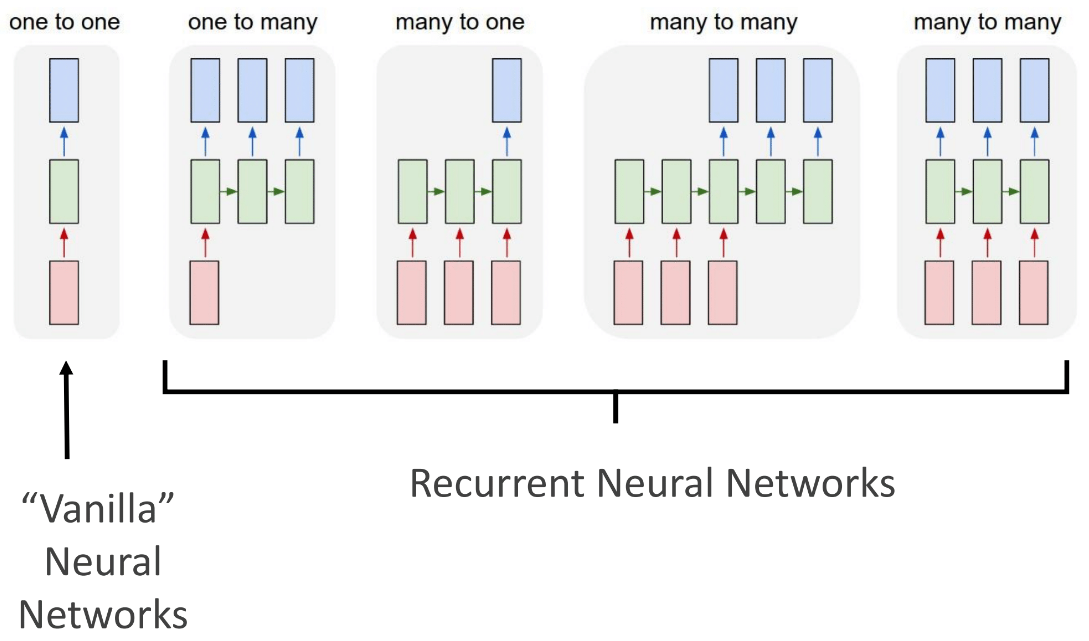
\includegraphics[scale=0.25]{img/NNs_vs_RNN.png}
    \caption{It is not limited to a fixed size of inputs and outputs.} 
    \label{fig:rnns}
  \end{figure}

  Now to build such a model where the input or output elements are unbounded, we must take advantage of \textit{weight sharing} (as seen in the CNN architecture) to control the size of our neural net. Furthermore, the fact that we should take in a sequence of inputs means that we may want to introduce some recursive structure in our neural net. Consider the classical form of a dynamical system driven by an external signal $\mathbf{x}$ as 
  \begin{equation}
    \mathbf{s}_t = f(\mathbf{s}_{t-1}, \mathbf{x}_t; \, \boldsymbol{\theta} )
  \end{equation}
  which defines a recurrent relationship. Similarly, we can write $\mathbf{h}$ to represent hidden neurons and write 
  \begin{equation}
    \mathbf{h}_t = f(\mathbf{h}_{t-1}, \mathbf{x}_t; \, \boldsymbol{\theta} )
  \end{equation}
  which indicates that the state of a hidden neuron is dependent on both the previous neuron and an input at time $t$. Through recursion, the hidden state $\mathbf{h}_t$ contains all information about the inputs $\mathbf{x}_1, \ldots, \mathbf{x}_t$ in the form of a complex function $\mathbf{g}$. 
  \begin{align}
      \mathbf{h}_t & = \mathbf{g}_t \big( \mathbf{x}_t, \mathbf{x}_{t - 1}, \ldots, \mathbf{x}_1 \big) \\
      & = f(\mathbf{h}_{t - 1}, \mathbf{x}_t; \, \boldsymbol{\theta}) 
  \end{align}
  The fact that we can factorize $\mathbf{g}_t$ into a repeated application of function $\mathbf{f}$ gives us two advantages: 
  \begin{enumerate}
      \item Regardless of the sequence length, the learned model always has the same input size because it is specified in terms of transition from one state to another state, rather than specified in terms of a variable-length history of states. 

      \item It is possible to use the same transition function $f$ with the same parameters at every time step. Since we do not have a growing number of parameters to optimize as our sequential data grows, training an RNN is still computationally feasible. 
  \end{enumerate}
  These two factors make it possible to learn a single model $f$ that operates on all time steps and all sequence lengths, rather than needing to learn a separate model $\mathbf{g}_t$ for all possible time steps. 

\subsection{Unidirectional RNNs}

  A single layer unidirectional RNN is a direct application of the idea mentioned in the previous section. We can first look at its computational graph 

  \begin{figure}[H]
    \centering 
    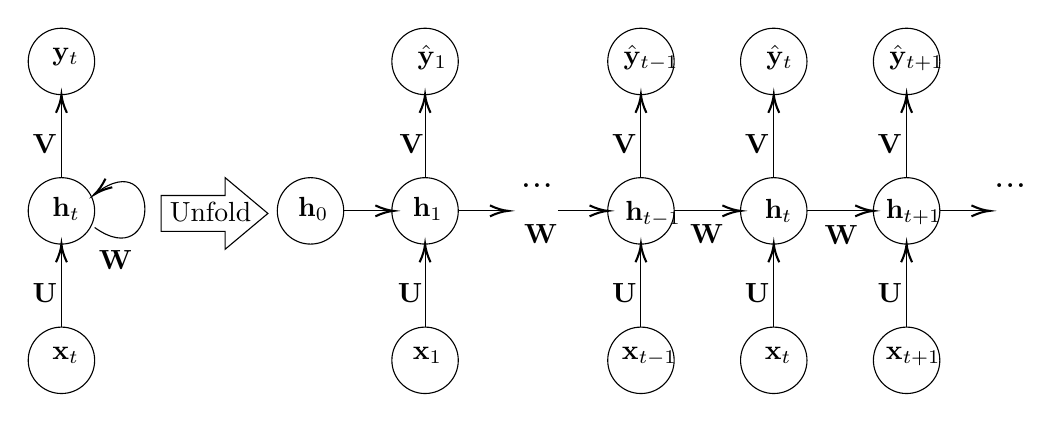
\begin{tikzpicture}[x=0.75pt,y=0.75pt,yscale=-0.8,xscale=0.8]
      %Shape: Ellipse [id:dp5130048407384993] 
      \draw   (40,30) .. controls (40,18.95) and (48.95,10) .. (60,10) .. controls (71.05,10) and (80,18.95) .. (80,30) .. controls (80,41.05) and (71.05,50) .. (60,50) .. controls (48.95,50) and (40,41.05) .. (40,30) -- cycle ;
      %Shape: Ellipse [id:dp17480372599276373] 
      \draw   (389,30) .. controls (389,18.95) and (397.95,10) .. (409,10) .. controls (420.05,10) and (429,18.95) .. (429,30) .. controls (429,41.05) and (420.05,50) .. (409,50) .. controls (397.95,50) and (389,41.05) .. (389,30) -- cycle ;
      %Shape: Ellipse [id:dp5960411091761506] 
      \draw   (549,30) .. controls (549,18.95) and (557.95,10) .. (569,10) .. controls (580.05,10) and (589,18.95) .. (589,30) .. controls (589,41.05) and (580.05,50) .. (569,50) .. controls (557.95,50) and (549,41.05) .. (549,30) -- cycle ;
      %Shape: Ellipse [id:dp7206562814926485] 
      \draw   (469,30) .. controls (469,18.95) and (477.95,10) .. (489,10) .. controls (500.05,10) and (509,18.95) .. (509,30) .. controls (509,41.05) and (500.05,50) .. (489,50) .. controls (477.95,50) and (469,41.05) .. (469,30) -- cycle ;
      %Curve Lines [id:da10598972243494376] 
      \draw [color={rgb, 255:red, 0; green, 0; blue, 0 }  ,draw opacity=1 ]   (80,130) .. controls (119.93,158.71) and (120.33,79.61) .. (81.2,109.07) ;
      \draw [shift={(80,110)}, rotate = 321.57] [color={rgb, 255:red, 0; green, 0; blue, 0 }  ,draw opacity=1 ][line width=0.75]    (10.93,-3.29) .. controls (6.95,-1.4) and (3.31,-0.3) .. (0,0) .. controls (3.31,0.3) and (6.95,1.4) .. (10.93,3.29)   ;
      %Right Arrow [id:dp18992895807915655] 
      \draw   (120,110.77) -- (158.6,110.77) -- (158.6,100) -- (184.34,121.55) -- (158.6,143.1) -- (158.6,132.32) -- (120,132.32) -- cycle ;
      %Shape: Ellipse [id:dp5707409054176504] 
      \draw   (40,120) .. controls (40,108.95) and (48.95,100) .. (60,100) .. controls (71.05,100) and (80,108.95) .. (80,120) .. controls (80,131.05) and (71.05,140) .. (60,140) .. controls (48.95,140) and (40,131.05) .. (40,120) -- cycle ;
      %Shape: Ellipse [id:dp7312065482605519] 
      \draw   (389,120) .. controls (389,108.95) and (397.95,100) .. (409,100) .. controls (420.05,100) and (429,108.95) .. (429,120) .. controls (429,131.05) and (420.05,140) .. (409,140) .. controls (397.95,140) and (389,131.05) .. (389,120) -- cycle ;
      %Shape: Ellipse [id:dp09029880081936525] 
      \draw   (549,120) .. controls (549,108.95) and (557.95,100) .. (569,100) .. controls (580.05,100) and (589,108.95) .. (589,120) .. controls (589,131.05) and (580.05,140) .. (569,140) .. controls (557.95,140) and (549,131.05) .. (549,120) -- cycle ;
      %Shape: Ellipse [id:dp3877188933189881] 
      \draw   (469,120) .. controls (469,108.95) and (477.95,100) .. (489,100) .. controls (500.05,100) and (509,108.95) .. (509,120) .. controls (509,131.05) and (500.05,140) .. (489,140) .. controls (477.95,140) and (469,131.05) .. (469,120) -- cycle ;
      %Shape: Ellipse [id:dp56230914391766] 
      \draw   (259,120) .. controls (259,108.95) and (267.95,100) .. (279,100) .. controls (290.05,100) and (299,108.95) .. (299,120) .. controls (299,131.05) and (290.05,140) .. (279,140) .. controls (267.95,140) and (259,131.05) .. (259,120) -- cycle ;
      %Straight Lines [id:da6793613738120752] 
      \draw [color={rgb, 255:red, 0; green, 0; blue, 0 }  ,draw opacity=1 ]   (299,120) -- (327,120) ;
      \draw [shift={(329,120)}, rotate = 180] [color={rgb, 255:red, 0; green, 0; blue, 0 }  ,draw opacity=1 ][line width=0.75]    (10.93,-3.29) .. controls (6.95,-1.4) and (3.31,-0.3) .. (0,0) .. controls (3.31,0.3) and (6.95,1.4) .. (10.93,3.29)   ;
      %Straight Lines [id:da07841792239013201] 
      \draw [color={rgb, 255:red, 0; green, 0; blue, 0 }  ,draw opacity=1 ]   (359,120) -- (387,120) ;
      \draw [shift={(389,120)}, rotate = 180] [color={rgb, 255:red, 0; green, 0; blue, 0 }  ,draw opacity=1 ][line width=0.75]    (10.93,-3.29) .. controls (6.95,-1.4) and (3.31,-0.3) .. (0,0) .. controls (3.31,0.3) and (6.95,1.4) .. (10.93,3.29)   ;
      %Straight Lines [id:da17044753691104964] 
      \draw [color={rgb, 255:red, 0; green, 0; blue, 0 }  ,draw opacity=1 ]   (429,120) -- (467,120) ;
      \draw [shift={(469,120)}, rotate = 180] [color={rgb, 255:red, 0; green, 0; blue, 0 }  ,draw opacity=1 ][line width=0.75]    (10.93,-3.29) .. controls (6.95,-1.4) and (3.31,-0.3) .. (0,0) .. controls (3.31,0.3) and (6.95,1.4) .. (10.93,3.29)   ;
      %Straight Lines [id:da6051247889848512] 
      \draw [color={rgb, 255:red, 0; green, 0; blue, 0 }  ,draw opacity=1 ]   (509,120) -- (547,120) ;
      \draw [shift={(549,120)}, rotate = 180] [color={rgb, 255:red, 0; green, 0; blue, 0 }  ,draw opacity=1 ][line width=0.75]    (10.93,-3.29) .. controls (6.95,-1.4) and (3.31,-0.3) .. (0,0) .. controls (3.31,0.3) and (6.95,1.4) .. (10.93,3.29)   ;
      %Straight Lines [id:da2538393669251706] 
      \draw [color={rgb, 255:red, 0; green, 0; blue, 0 }  ,draw opacity=1 ]   (589,120) -- (617,120) ;
      \draw [shift={(619,120)}, rotate = 180] [color={rgb, 255:red, 0; green, 0; blue, 0 }  ,draw opacity=1 ][line width=0.75]    (10.93,-3.29) .. controls (6.95,-1.4) and (3.31,-0.3) .. (0,0) .. controls (3.31,0.3) and (6.95,1.4) .. (10.93,3.29)   ;
      %Shape: Ellipse [id:dp6518089160353446] 
      \draw   (40,210) .. controls (40,198.95) and (48.95,190) .. (60,190) .. controls (71.05,190) and (80,198.95) .. (80,210) .. controls (80,221.05) and (71.05,230) .. (60,230) .. controls (48.95,230) and (40,221.05) .. (40,210) -- cycle ;
      %Shape: Ellipse [id:dp8865546010531642] 
      \draw   (389,210) .. controls (389,198.95) and (397.95,190) .. (409,190) .. controls (420.05,190) and (429,198.95) .. (429,210) .. controls (429,221.05) and (420.05,230) .. (409,230) .. controls (397.95,230) and (389,221.05) .. (389,210) -- cycle ;
      %Shape: Ellipse [id:dp9568354714915992] 
      \draw   (549,210) .. controls (549,198.95) and (557.95,190) .. (569,190) .. controls (580.05,190) and (589,198.95) .. (589,210) .. controls (589,221.05) and (580.05,230) .. (569,230) .. controls (557.95,230) and (549,221.05) .. (549,210) -- cycle ;
      %Shape: Ellipse [id:dp5199285238560907] 
      \draw   (469,210) .. controls (469,198.95) and (477.95,190) .. (489,190) .. controls (500.05,190) and (509,198.95) .. (509,210) .. controls (509,221.05) and (500.05,230) .. (489,230) .. controls (477.95,230) and (469,221.05) .. (469,210) -- cycle ;
      %Shape: Ellipse [id:dp5177448938556457] 
      \draw   (259,210) .. controls (259,198.95) and (267.95,190) .. (279,190) .. controls (290.05,190) and (299,198.95) .. (299,210) .. controls (299,221.05) and (290.05,230) .. (279,230) .. controls (267.95,230) and (259,221.05) .. (259,210) -- cycle ;
      %Straight Lines [id:da48553186555219585] 
      \draw [color={rgb, 255:red, 0; green, 0; blue, 0 }  ,draw opacity=1 ]   (279,190) -- (279,142) ;
      \draw [shift={(279,140)}, rotate = 90] [color={rgb, 255:red, 0; green, 0; blue, 0 }  ,draw opacity=1 ][line width=0.75]    (10.93,-3.29) .. controls (6.95,-1.4) and (3.31,-0.3) .. (0,0) .. controls (3.31,0.3) and (6.95,1.4) .. (10.93,3.29)   ;
      %Straight Lines [id:da2936880234308463] 
      \draw [color={rgb, 255:red, 0; green, 0; blue, 0 }  ,draw opacity=1 ]   (409,100) -- (409,52) ;
      \draw [shift={(409,50)}, rotate = 90] [color={rgb, 255:red, 0; green, 0; blue, 0 }  ,draw opacity=1 ][line width=0.75]    (10.93,-3.29) .. controls (6.95,-1.4) and (3.31,-0.3) .. (0,0) .. controls (3.31,0.3) and (6.95,1.4) .. (10.93,3.29)   ;
      %Straight Lines [id:da9311498223018868] 
      \draw [color={rgb, 255:red, 0; green, 0; blue, 0 }  ,draw opacity=1 ]   (409,190) -- (409,142) ;
      \draw [shift={(409,140)}, rotate = 90] [color={rgb, 255:red, 0; green, 0; blue, 0 }  ,draw opacity=1 ][line width=0.75]    (10.93,-3.29) .. controls (6.95,-1.4) and (3.31,-0.3) .. (0,0) .. controls (3.31,0.3) and (6.95,1.4) .. (10.93,3.29)   ;
      %Straight Lines [id:da8567250362301639] 
      \draw [color={rgb, 255:red, 0; green, 0; blue, 0 }  ,draw opacity=1 ]   (489,100) -- (489,66) -- (489,52) ;
      \draw [shift={(489,50)}, rotate = 90] [color={rgb, 255:red, 0; green, 0; blue, 0 }  ,draw opacity=1 ][line width=0.75]    (10.93,-3.29) .. controls (6.95,-1.4) and (3.31,-0.3) .. (0,0) .. controls (3.31,0.3) and (6.95,1.4) .. (10.93,3.29)   ;
      %Straight Lines [id:da8233396894283387] 
      \draw [color={rgb, 255:red, 0; green, 0; blue, 0 }  ,draw opacity=1 ]   (489,190) -- (489,142) ;
      \draw [shift={(489,140)}, rotate = 90] [color={rgb, 255:red, 0; green, 0; blue, 0 }  ,draw opacity=1 ][line width=0.75]    (10.93,-3.29) .. controls (6.95,-1.4) and (3.31,-0.3) .. (0,0) .. controls (3.31,0.3) and (6.95,1.4) .. (10.93,3.29)   ;
      %Straight Lines [id:da1927225854059864] 
      \draw [color={rgb, 255:red, 0; green, 0; blue, 0 }  ,draw opacity=1 ]   (569,100) -- (569,52) ;
      \draw [shift={(569,50)}, rotate = 90] [color={rgb, 255:red, 0; green, 0; blue, 0 }  ,draw opacity=1 ][line width=0.75]    (10.93,-3.29) .. controls (6.95,-1.4) and (3.31,-0.3) .. (0,0) .. controls (3.31,0.3) and (6.95,1.4) .. (10.93,3.29)   ;
      %Straight Lines [id:da07289599684208947] 
      \draw [color={rgb, 255:red, 0; green, 0; blue, 0 }  ,draw opacity=1 ]   (569,190) -- (569,142) ;
      \draw [shift={(569,140)}, rotate = 90] [color={rgb, 255:red, 0; green, 0; blue, 0 }  ,draw opacity=1 ][line width=0.75]    (10.93,-3.29) .. controls (6.95,-1.4) and (3.31,-0.3) .. (0,0) .. controls (3.31,0.3) and (6.95,1.4) .. (10.93,3.29)   ;
      %Straight Lines [id:da8826756188793603] 
      \draw [color={rgb, 255:red, 0; green, 0; blue, 0 }  ,draw opacity=1 ]   (60,100) -- (60,52) ;
      \draw [shift={(60,50)}, rotate = 90] [color={rgb, 255:red, 0; green, 0; blue, 0 }  ,draw opacity=1 ][line width=0.75]    (10.93,-3.29) .. controls (6.95,-1.4) and (3.31,-0.3) .. (0,0) .. controls (3.31,0.3) and (6.95,1.4) .. (10.93,3.29)   ;
      %Straight Lines [id:da41048676999998257] 
      \draw [color={rgb, 255:red, 0; green, 0; blue, 0 }  ,draw opacity=1 ]   (60,190) -- (60,142) ;
      \draw [shift={(60,140)}, rotate = 90] [color={rgb, 255:red, 0; green, 0; blue, 0 }  ,draw opacity=1 ][line width=0.75]    (10.93,-3.29) .. controls (6.95,-1.4) and (3.31,-0.3) .. (0,0) .. controls (3.31,0.3) and (6.95,1.4) .. (10.93,3.29)   ;
      %Shape: Ellipse [id:dp4446219054358924] 
      \draw   (259,30) .. controls (259,18.95) and (267.95,10) .. (279,10) .. controls (290.05,10) and (299,18.95) .. (299,30) .. controls (299,41.05) and (290.05,50) .. (279,50) .. controls (267.95,50) and (259,41.05) .. (259,30) -- cycle ;
      %Straight Lines [id:da4580075835908557] 
      \draw [color={rgb, 255:red, 0; green, 0; blue, 0 }  ,draw opacity=1 ]   (279,100) -- (279,66) -- (279,52) ;
      \draw [shift={(279,50)}, rotate = 90] [color={rgb, 255:red, 0; green, 0; blue, 0 }  ,draw opacity=1 ][line width=0.75]    (10.93,-3.29) .. controls (6.95,-1.4) and (3.31,-0.3) .. (0,0) .. controls (3.31,0.3) and (6.95,1.4) .. (10.93,3.29)   ;
      %Shape: Ellipse [id:dp6113115655399299] 
      \draw   (190,120) .. controls (190,108.95) and (198.95,100) .. (210,100) .. controls (221.05,100) and (230,108.95) .. (230,120) .. controls (230,131.05) and (221.05,140) .. (210,140) .. controls (198.95,140) and (190,131.05) .. (190,120) -- cycle ;
      %Straight Lines [id:da5578894272255863] 
      \draw [color={rgb, 255:red, 0; green, 0; blue, 0 }  ,draw opacity=1 ]   (230,120) -- (258,120) ;
      \draw [shift={(260,120)}, rotate = 180] [color={rgb, 255:red, 0; green, 0; blue, 0 }  ,draw opacity=1 ][line width=0.75]    (10.93,-3.29) .. controls (6.95,-1.4) and (3.31,-0.3) .. (0,0) .. controls (3.31,0.3) and (6.95,1.4) .. (10.93,3.29)   ;

      % Text Node
      \draw (335,102) node [anchor=north west][inner sep=0.75pt]  [font=\Large] [align=left] {...};
      % Text Node
      \draw (397,18.4) node [anchor=north west][inner sep=0.75pt]  [font=\normalsize]  {$\hat{\mathbf{y}}_{t-1}$};
      % Text Node
      \draw (123.69,113.09) node [anchor=north west][inner sep=0.75pt]   [align=left] {Unfold};
      % Text Node
      \draw (337,126.4) node [anchor=north west][inner sep=0.75pt]  [font=\normalsize,color={rgb, 255:red, 0; green, 0; blue, 0 }  ,opacity=1 ]  {$\mathbf{W}$};
      % Text Node
      \draw (53,20.4) node [anchor=north west][inner sep=0.75pt]  [font=\normalsize]  {$\mathbf{y}_{t}$};
      % Text Node
      \draw (270,110.4) node [anchor=north west][inner sep=0.75pt]  [font=\normalsize]  {$\mathbf{h}_{1}$};
      % Text Node
      \draw (398,112.4) node [anchor=north west][inner sep=0.75pt]  [font=\normalsize]  {$\mathbf{h}_{t-1}$};
      % Text Node
      \draw (482,111.4) node [anchor=north west][inner sep=0.75pt]  [font=\normalsize]  {$\mathbf{h}_{t}$};
      % Text Node
      \draw (555,111.4) node [anchor=north west][inner sep=0.75pt]  [font=\normalsize]  {$\mathbf{h}_{t+1}$};
      % Text Node
      \draw (53,110.4) node [anchor=north west][inner sep=0.75pt]  [font=\normalsize]  {$\mathbf{h}_{t}$};
      % Text Node
      \draw (620,102) node [anchor=north west][inner sep=0.75pt]  [font=\Large] [align=left] {...};
      % Text Node
      \draw (437,126.4) node [anchor=north west][inner sep=0.75pt]  [font=\normalsize,color={rgb, 255:red, 0; green, 0; blue, 0 }  ,opacity=1 ]  {$\mathbf{W}$};
      % Text Node
      \draw (270,200.4) node [anchor=north west][inner sep=0.75pt]  [font=\normalsize]  {$\mathbf{x}_{1}$};
      % Text Node
      \draw (396,200.4) node [anchor=north west][inner sep=0.75pt]  [font=\normalsize]  {$\mathbf{x}_{t-1}$};
      % Text Node
      \draw (482,200.4) node [anchor=north west][inner sep=0.75pt]  [font=\normalsize]  {$\mathbf{x}_{t}$};
      % Text Node
      \draw (555,200.4) node [anchor=north west][inner sep=0.75pt]  [font=\normalsize]  {$\mathbf{x}_{t+1}$};
      % Text Node
      \draw (53,200.4) node [anchor=north west][inner sep=0.75pt]  [font=\normalsize]  {$\mathbf{x}_{t}$};
      % Text Node
      \draw (261,162.4) node [anchor=north west][inner sep=0.75pt]  [font=\normalsize,color={rgb, 255:red, 0; green, 0; blue, 0 }  ,opacity=1 ]  {$\mathbf{U}$};
      % Text Node
      \draw (81,142.4) node [anchor=north west][inner sep=0.75pt]  [font=\normalsize,color={rgb, 255:red, 0; green, 0; blue, 0 }  ,opacity=1 ]  {$\mathbf{W}$};
      % Text Node
      \draw (390,72.4) node [anchor=north west][inner sep=0.75pt]  [font=\normalsize,color={rgb, 255:red, 0; green, 0; blue, 0 }  ,opacity=1 ]  {$\mathbf{V}$};
      % Text Node
      \draw (390,162.4) node [anchor=north west][inner sep=0.75pt]  [font=\normalsize,color={rgb, 255:red, 0; green, 0; blue, 0 }  ,opacity=1 ]  {$\mathbf{U}$};
      % Text Node
      \draw (470,72.4) node [anchor=north west][inner sep=0.75pt]  [font=\normalsize,color={rgb, 255:red, 0; green, 0; blue, 0 }  ,opacity=1 ]  {$\mathbf{V}$};
      % Text Node
      \draw (470,162.4) node [anchor=north west][inner sep=0.75pt]  [font=\normalsize,color={rgb, 255:red, 0; green, 0; blue, 0 }  ,opacity=1 ]  {$\mathbf{U}$};
      % Text Node
      \draw (550,72.4) node [anchor=north west][inner sep=0.75pt]  [font=\normalsize,color={rgb, 255:red, 0; green, 0; blue, 0 }  ,opacity=1 ]  {$\mathbf{V}$};
      % Text Node
      \draw (550,162.4) node [anchor=north west][inner sep=0.75pt]  [font=\normalsize,color={rgb, 255:red, 0; green, 0; blue, 0 }  ,opacity=1 ]  {$\mathbf{U}$};
      % Text Node
      \draw (41,72.4) node [anchor=north west][inner sep=0.75pt]  [font=\normalsize,color={rgb, 255:red, 0; green, 0; blue, 0 }  ,opacity=1 ]  {$\mathbf{V}$};
      % Text Node
      \draw (41,162.4) node [anchor=north west][inner sep=0.75pt]  [font=\normalsize,color={rgb, 255:red, 0; green, 0; blue, 0 }  ,opacity=1 ]  {$\mathbf{U}$};
      % Text Node
      \draw (518,127.4) node [anchor=north west][inner sep=0.75pt]  [font=\normalsize,color={rgb, 255:red, 0; green, 0; blue, 0 }  ,opacity=1 ]  {$\mathbf{W}$};
      % Text Node
      \draw (483,18.4) node [anchor=north west][inner sep=0.75pt]  [font=\normalsize]  {$\hat{\mathbf{y}}_{t}$};
      % Text Node
      \draw (557,18.4) node [anchor=north west][inner sep=0.75pt]  [font=\normalsize]  {$\hat{\mathbf{y}}_{t+1}$};
      % Text Node
      \draw (262,72.4) node [anchor=north west][inner sep=0.75pt]  [font=\normalsize,color={rgb, 255:red, 0; green, 0; blue, 0 }  ,opacity=1 ]  {$\mathbf{V}$};
      % Text Node
      \draw (273,18.4) node [anchor=north west][inner sep=0.75pt]  [font=\normalsize]  {$\hat{\mathbf{y}}_{1}$};
      % Text Node
      \draw (201,110.4) node [anchor=north west][inner sep=0.75pt]  [font=\normalsize]  {$\mathbf{h}_{0}$};
    \end{tikzpicture}
    \caption{The circular arrow is notation for an RNN that ``unfolds'' to the graph on the right. } 
    \label{fig:one_layer_rnn}
  \end{figure}

  The activation functions that map to the hidden nodes and the outputs will be labeled $\boldsymbol{\sigma}_{h}$ and $\boldsymbol{\sigma}_{y}$, respectively. In general the $W$ will represent the left and right mappings between hidden nodes, the $U$ will represent the map going up from the input or hidden node to a hidden node, and $V$ is the final mapping from a hidden node to an output. We only label the arrows with the matrices, though a bias term and the nonlinear activation function are still there. That is, we can summarize our network as
  \begin{align}
    \mathbf{h}_t & = \mathbf{f}( \mathbf{h}_{t - 1}, \mathbf{x}_{t} ; \, \boldsymbol{\theta}) = \boldsymbol{\sigma}_h \big( \mathbf{W} \mathbf{h}_{t - 1} + \mathbf{U} \mathbf{x}_t + \mathbf{b}_h \big) \\
    \mathbf{y}_t & = \boldsymbol{\sigma}_y \big( \mathbf{V} \mathbf{h}_t + \mathbf{b}_y \big) 
  \end{align}
  for $t = 1, \ldots, \tau$, where $\mathbf{h}_0$ is initialized to be zeroes or some small vector. The dimensions of the maps and the variables are listed for clarification: 
  \begin{enumerate}
    \item $\mathbf{x}_t \in \mathbb{R}^d$ for all $t$
    \item $\mathbf{h}_t \in \mathbb{R}^h$ for all $t$
    \item $\mathbf{b}_h \in \mathbb{R}^h$
    \item $\mathbf{U} \in \mathbb{R}^{h \times d}$
    \item $\mathbf{W} \in \mathbb{R}^{h \times h}$
  \end{enumerate}
  As we can see, the hidden node from the previous time step provides a form of memory, or context, that encodes earlier processing and informs the decisions to be made at later points in time. Adding this temporal dimension makes RNNs appear to be more complex than non-recurrent architectures, but in reality, they’re not all that different. Consider the rearranged architecture of an RNN below. 

  \begin{figure}[H]
    \centering 
    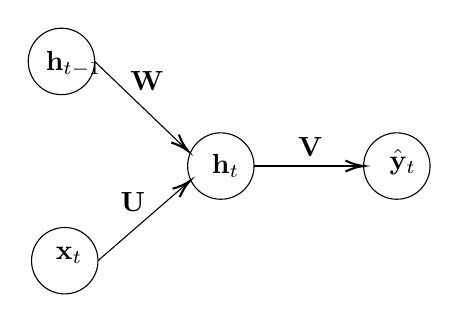
\begin{tikzpicture}[x=0.75pt,y=0.75pt,yscale=-0.8,xscale=0.8]
      %Shape: Ellipse [id:dp9795697082977448] 
      \draw   (412,88.33) .. controls (412,77.29) and (420.95,68.33) .. (432,68.33) .. controls (443.05,68.33) and (452,77.29) .. (452,88.33) .. controls (452,99.38) and (443.05,108.33) .. (432,108.33) .. controls (420.95,108.33) and (412,99.38) .. (412,88.33) -- cycle ;
      %Shape: Ellipse [id:dp8435868286837831] 
      \draw   (210,25.33) .. controls (210,14.29) and (218.95,5.33) .. (230,5.33) .. controls (241.05,5.33) and (250,14.29) .. (250,25.33) .. controls (250,36.38) and (241.05,45.33) .. (230,45.33) .. controls (218.95,45.33) and (210,36.38) .. (210,25.33) -- cycle ;
      %Shape: Ellipse [id:dp10562076709489165] 
      \draw   (306,88.33) .. controls (306,77.29) and (314.95,68.33) .. (326,68.33) .. controls (337.05,68.33) and (346,77.29) .. (346,88.33) .. controls (346,99.38) and (337.05,108.33) .. (326,108.33) .. controls (314.95,108.33) and (306,99.38) .. (306,88.33) -- cycle ;
      %Straight Lines [id:da00030920510583576366] 
      \draw [color={rgb, 255:red, 0; green, 0; blue, 0 }  ,draw opacity=1 ]   (250,25.33) -- (304.89,77.95) ;
      \draw [shift={(306.33,79.33)}, rotate = 223.79] [color={rgb, 255:red, 0; green, 0; blue, 0 }  ,draw opacity=1 ][line width=0.75]    (10.93,-3.29) .. controls (6.95,-1.4) and (3.31,-0.3) .. (0,0) .. controls (3.31,0.3) and (6.95,1.4) .. (10.93,3.29)   ;
      %Shape: Ellipse [id:dp611931387208084] 
      \draw   (212,145.33) .. controls (212,134.29) and (220.95,125.33) .. (232,125.33) .. controls (243.05,125.33) and (252,134.29) .. (252,145.33) .. controls (252,156.38) and (243.05,165.33) .. (232,165.33) .. controls (220.95,165.33) and (212,156.38) .. (212,145.33) -- cycle ;
      %Straight Lines [id:da04817982276379906] 
      \draw [color={rgb, 255:red, 0; green, 0; blue, 0 }  ,draw opacity=1 ]   (252,145.33) -- (305.82,98.64) ;
      \draw [shift={(307.33,97.33)}, rotate = 139.06] [color={rgb, 255:red, 0; green, 0; blue, 0 }  ,draw opacity=1 ][line width=0.75]    (10.93,-3.29) .. controls (6.95,-1.4) and (3.31,-0.3) .. (0,0) .. controls (3.31,0.3) and (6.95,1.4) .. (10.93,3.29)   ;
      %Straight Lines [id:da9431583172236413] 
      \draw [color={rgb, 255:red, 0; green, 0; blue, 0 }  ,draw opacity=1 ]   (346,88.33) -- (410,88.33) ;
      \draw [shift={(412,88.33)}, rotate = 180] [color={rgb, 255:red, 0; green, 0; blue, 0 }  ,draw opacity=1 ][line width=0.75]    (10.93,-3.29) .. controls (6.95,-1.4) and (3.31,-0.3) .. (0,0) .. controls (3.31,0.3) and (6.95,1.4) .. (10.93,3.29)   ;

      % Text Node
      \draw (219,17.73) node [anchor=north west][inner sep=0.75pt]  [font=\normalsize]  {$\mathbf{h}_{t-1}$};
      % Text Node
      \draw (319,79.73) node [anchor=north west][inner sep=0.75pt]  [font=\normalsize]  {$\mathbf{h}_{t}$};
      % Text Node
      \draw (270,29.73) node [anchor=north west][inner sep=0.75pt]  [font=\normalsize,color={rgb, 255:red, 0; green, 0; blue, 0 }  ,opacity=1 ]  {$\mathbf{W}$};
      % Text Node
      \draw (225,135.73) node [anchor=north west][inner sep=0.75pt]  [font=\normalsize]  {$\mathbf{x}_{t}$};
      % Text Node
      \draw (371,69.73) node [anchor=north west][inner sep=0.75pt]  [font=\normalsize,color={rgb, 255:red, 0; green, 0; blue, 0 }  ,opacity=1 ]  {$\mathbf{V}$};
      % Text Node
      \draw (264,102.73) node [anchor=north west][inner sep=0.75pt]  [font=\normalsize,color={rgb, 255:red, 0; green, 0; blue, 0 }  ,opacity=1 ]  {$\mathbf{U}$};
      % Text Node
      \draw (426,76.73) node [anchor=north west][inner sep=0.75pt]  [font=\normalsize]  {$\hat{\mathbf{y}}_{t}$};
    \end{tikzpicture}
    \caption{RNNs as an MLP. } 
    \label{fig:mlp_vs_rnn}
  \end{figure}

  \subsubsection{Loss Functions}

    The form of the loss for a RNN will have to be slightly modified, since we can have multiple outputs. If we have a given input-output pair $\mathbf{x}^{(n)}, \mathbf{y}^{(n)}$, and we are interested producing a single output, then this is similar to what we already do with regular NNs. If we are interested in producing a sequence of outputs, then we can average the loss functions individually so that equal weight is placed on the prediction at each relevant timestep. This is called 
    \begin{equation}
      L = \frac{1}{|T|} \sum_{t \in T} L_t
    \end{equation}
    Sometimes, even with single inputs it may be good to include other intermediate terms in the loss so that we can direct the neural net to converge faster to what the correct answer should be. 

    \begin{figure}[H]
      \centering 
      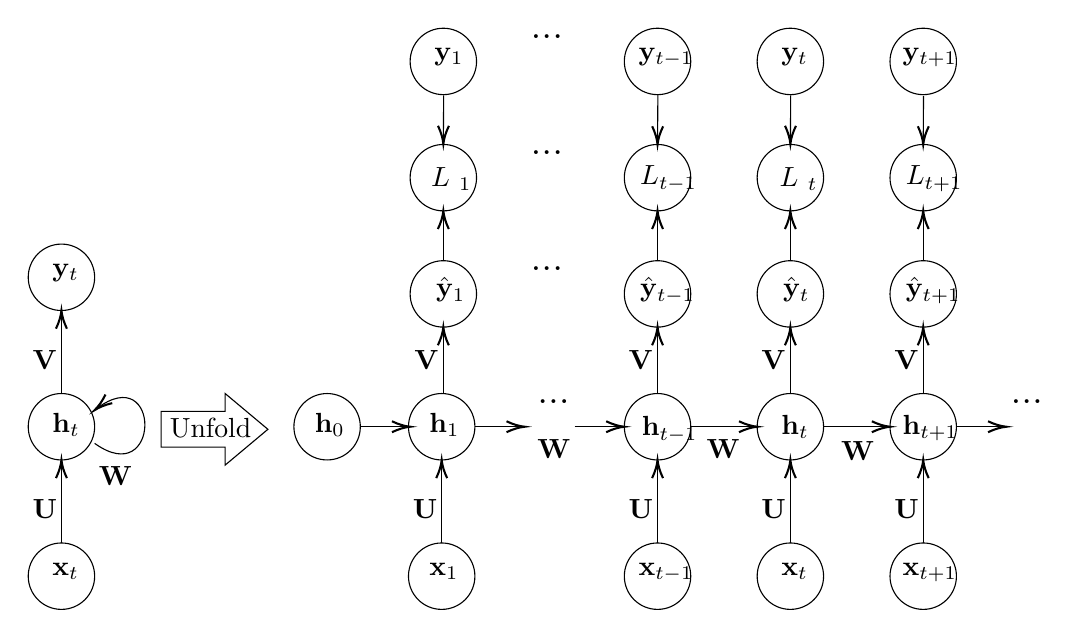
\begin{tikzpicture}[x=0.75pt,y=0.75pt,yscale=-0.8,xscale=0.8]
        %Shape: Ellipse [id:dp9680953270479153] 
        \draw   (30,160) .. controls (30,148.95) and (38.95,140) .. (50,140) .. controls (61.05,140) and (70,148.95) .. (70,160) .. controls (70,171.05) and (61.05,180) .. (50,180) .. controls (38.95,180) and (30,171.05) .. (30,160) -- cycle ;
        %Shape: Ellipse [id:dp5730005571966859] 
        \draw   (389,170) .. controls (389,158.95) and (397.95,150) .. (409,150) .. controls (420.05,150) and (429,158.95) .. (429,170) .. controls (429,181.05) and (420.05,190) .. (409,190) .. controls (397.95,190) and (389,181.05) .. (389,170) -- cycle ;
        %Shape: Ellipse [id:dp4570036898065337] 
        \draw   (549,170) .. controls (549,158.95) and (557.95,150) .. (569,150) .. controls (580.05,150) and (589,158.95) .. (589,170) .. controls (589,181.05) and (580.05,190) .. (569,190) .. controls (557.95,190) and (549,181.05) .. (549,170) -- cycle ;
        %Shape: Ellipse [id:dp310472974621425] 
        \draw   (469,170) .. controls (469,158.95) and (477.95,150) .. (489,150) .. controls (500.05,150) and (509,158.95) .. (509,170) .. controls (509,181.05) and (500.05,190) .. (489,190) .. controls (477.95,190) and (469,181.05) .. (469,170) -- cycle ;
        %Curve Lines [id:da9737186251466903] 
        \draw [color={rgb, 255:red, 0; green, 0; blue, 0 }  ,draw opacity=1 ]   (70,260) .. controls (109.93,288.71) and (110.33,209.61) .. (71.2,239.07) ;
        \draw [shift={(70,240)}, rotate = 321.57] [color={rgb, 255:red, 0; green, 0; blue, 0 }  ,draw opacity=1 ][line width=0.75]    (10.93,-3.29) .. controls (6.95,-1.4) and (3.31,-0.3) .. (0,0) .. controls (3.31,0.3) and (6.95,1.4) .. (10.93,3.29)   ;
        %Right Arrow [id:dp7863084495909953] 
        \draw   (110,240.77) -- (148.6,240.77) -- (148.6,230) -- (174.34,251.55) -- (148.6,273.1) -- (148.6,262.32) -- (110,262.32) -- cycle ;
        %Shape: Ellipse [id:dp6734347060174906] 
        \draw   (30,250) .. controls (30,238.95) and (38.95,230) .. (50,230) .. controls (61.05,230) and (70,238.95) .. (70,250) .. controls (70,261.05) and (61.05,270) .. (50,270) .. controls (38.95,270) and (30,261.05) .. (30,250) -- cycle ;
        %Shape: Ellipse [id:dp7555672305174788] 
        \draw   (389,250) .. controls (389,238.95) and (397.95,230) .. (409,230) .. controls (420.05,230) and (429,238.95) .. (429,250) .. controls (429,261.05) and (420.05,270) .. (409,270) .. controls (397.95,270) and (389,261.05) .. (389,250) -- cycle ;
        %Shape: Ellipse [id:dp8969160954412736] 
        \draw   (549,250) .. controls (549,238.95) and (557.95,230) .. (569,230) .. controls (580.05,230) and (589,238.95) .. (589,250) .. controls (589,261.05) and (580.05,270) .. (569,270) .. controls (557.95,270) and (549,261.05) .. (549,250) -- cycle ;
        %Shape: Ellipse [id:dp5010811857470736] 
        \draw   (469,250) .. controls (469,238.95) and (477.95,230) .. (489,230) .. controls (500.05,230) and (509,238.95) .. (509,250) .. controls (509,261.05) and (500.05,270) .. (489,270) .. controls (477.95,270) and (469,261.05) .. (469,250) -- cycle ;
        %Shape: Ellipse [id:dp15020874314124955] 
        \draw   (259,250) .. controls (259,238.95) and (267.95,230) .. (279,230) .. controls (290.05,230) and (299,238.95) .. (299,250) .. controls (299,261.05) and (290.05,270) .. (279,270) .. controls (267.95,270) and (259,261.05) .. (259,250) -- cycle ;
        %Straight Lines [id:da9739407532599313] 
        \draw [color={rgb, 255:red, 0; green, 0; blue, 0 }  ,draw opacity=1 ]   (299,250) -- (327,250) ;
        \draw [shift={(329,250)}, rotate = 180] [color={rgb, 255:red, 0; green, 0; blue, 0 }  ,draw opacity=1 ][line width=0.75]    (10.93,-3.29) .. controls (6.95,-1.4) and (3.31,-0.3) .. (0,0) .. controls (3.31,0.3) and (6.95,1.4) .. (10.93,3.29)   ;
        %Straight Lines [id:da42172683153715984] 
        \draw [color={rgb, 255:red, 0; green, 0; blue, 0 }  ,draw opacity=1 ]   (359,250) -- (387,250) ;
        \draw [shift={(389,250)}, rotate = 180] [color={rgb, 255:red, 0; green, 0; blue, 0 }  ,draw opacity=1 ][line width=0.75]    (10.93,-3.29) .. controls (6.95,-1.4) and (3.31,-0.3) .. (0,0) .. controls (3.31,0.3) and (6.95,1.4) .. (10.93,3.29)   ;
        %Straight Lines [id:da6928721729158405] 
        \draw [color={rgb, 255:red, 0; green, 0; blue, 0 }  ,draw opacity=1 ]   (429,250) -- (467,250) ;
        \draw [shift={(469,250)}, rotate = 180] [color={rgb, 255:red, 0; green, 0; blue, 0 }  ,draw opacity=1 ][line width=0.75]    (10.93,-3.29) .. controls (6.95,-1.4) and (3.31,-0.3) .. (0,0) .. controls (3.31,0.3) and (6.95,1.4) .. (10.93,3.29)   ;
        %Straight Lines [id:da9699219090048701] 
        \draw [color={rgb, 255:red, 0; green, 0; blue, 0 }  ,draw opacity=1 ]   (509,250) -- (547,250) ;
        \draw [shift={(549,250)}, rotate = 180] [color={rgb, 255:red, 0; green, 0; blue, 0 }  ,draw opacity=1 ][line width=0.75]    (10.93,-3.29) .. controls (6.95,-1.4) and (3.31,-0.3) .. (0,0) .. controls (3.31,0.3) and (6.95,1.4) .. (10.93,3.29)   ;
        %Straight Lines [id:da9089120498679435] 
        \draw [color={rgb, 255:red, 0; green, 0; blue, 0 }  ,draw opacity=1 ]   (589,250) -- (617,250) ;
        \draw [shift={(619,250)}, rotate = 180] [color={rgb, 255:red, 0; green, 0; blue, 0 }  ,draw opacity=1 ][line width=0.75]    (10.93,-3.29) .. controls (6.95,-1.4) and (3.31,-0.3) .. (0,0) .. controls (3.31,0.3) and (6.95,1.4) .. (10.93,3.29)   ;
        %Shape: Ellipse [id:dp2664716169413004] 
        \draw   (30,340) .. controls (30,328.95) and (38.95,320) .. (50,320) .. controls (61.05,320) and (70,328.95) .. (70,340) .. controls (70,351.05) and (61.05,360) .. (50,360) .. controls (38.95,360) and (30,351.05) .. (30,340) -- cycle ;
        %Shape: Ellipse [id:dp9588931299107948] 
        \draw   (389,340) .. controls (389,328.95) and (397.95,320) .. (409,320) .. controls (420.05,320) and (429,328.95) .. (429,340) .. controls (429,351.05) and (420.05,360) .. (409,360) .. controls (397.95,360) and (389,351.05) .. (389,340) -- cycle ;
        %Shape: Ellipse [id:dp011971914379850457] 
        \draw   (549,340) .. controls (549,328.95) and (557.95,320) .. (569,320) .. controls (580.05,320) and (589,328.95) .. (589,340) .. controls (589,351.05) and (580.05,360) .. (569,360) .. controls (557.95,360) and (549,351.05) .. (549,340) -- cycle ;
        %Shape: Ellipse [id:dp9234187724355627] 
        \draw   (469,340) .. controls (469,328.95) and (477.95,320) .. (489,320) .. controls (500.05,320) and (509,328.95) .. (509,340) .. controls (509,351.05) and (500.05,360) .. (489,360) .. controls (477.95,360) and (469,351.05) .. (469,340) -- cycle ;
        %Shape: Ellipse [id:dp32361468564640217] 
        \draw   (259,340) .. controls (259,328.95) and (267.95,320) .. (279,320) .. controls (290.05,320) and (299,328.95) .. (299,340) .. controls (299,351.05) and (290.05,360) .. (279,360) .. controls (267.95,360) and (259,351.05) .. (259,340) -- cycle ;
        %Straight Lines [id:da17794535301053505] 
        \draw [color={rgb, 255:red, 0; green, 0; blue, 0 }  ,draw opacity=1 ]   (279,320) -- (279,272) ;
        \draw [shift={(279,270)}, rotate = 90] [color={rgb, 255:red, 0; green, 0; blue, 0 }  ,draw opacity=1 ][line width=0.75]    (10.93,-3.29) .. controls (6.95,-1.4) and (3.31,-0.3) .. (0,0) .. controls (3.31,0.3) and (6.95,1.4) .. (10.93,3.29)   ;
        %Straight Lines [id:da39434249393019916] 
        \draw [color={rgb, 255:red, 0; green, 0; blue, 0 }  ,draw opacity=1 ]   (409,230) -- (409,192) ;
        \draw [shift={(409,190)}, rotate = 90] [color={rgb, 255:red, 0; green, 0; blue, 0 }  ,draw opacity=1 ][line width=0.75]    (10.93,-3.29) .. controls (6.95,-1.4) and (3.31,-0.3) .. (0,0) .. controls (3.31,0.3) and (6.95,1.4) .. (10.93,3.29)   ;
        %Straight Lines [id:da8293325821143183] 
        \draw [color={rgb, 255:red, 0; green, 0; blue, 0 }  ,draw opacity=1 ]   (409,320) -- (409,272) ;
        \draw [shift={(409,270)}, rotate = 90] [color={rgb, 255:red, 0; green, 0; blue, 0 }  ,draw opacity=1 ][line width=0.75]    (10.93,-3.29) .. controls (6.95,-1.4) and (3.31,-0.3) .. (0,0) .. controls (3.31,0.3) and (6.95,1.4) .. (10.93,3.29)   ;
        %Straight Lines [id:da22535194171078898] 
        \draw [color={rgb, 255:red, 0; green, 0; blue, 0 }  ,draw opacity=1 ]   (489,230) -- (489,196) -- (489,192) ;
        \draw [shift={(489,190)}, rotate = 90] [color={rgb, 255:red, 0; green, 0; blue, 0 }  ,draw opacity=1 ][line width=0.75]    (10.93,-3.29) .. controls (6.95,-1.4) and (3.31,-0.3) .. (0,0) .. controls (3.31,0.3) and (6.95,1.4) .. (10.93,3.29)   ;
        %Straight Lines [id:da22035114948288692] 
        \draw [color={rgb, 255:red, 0; green, 0; blue, 0 }  ,draw opacity=1 ]   (489,320) -- (489,272) ;
        \draw [shift={(489,270)}, rotate = 90] [color={rgb, 255:red, 0; green, 0; blue, 0 }  ,draw opacity=1 ][line width=0.75]    (10.93,-3.29) .. controls (6.95,-1.4) and (3.31,-0.3) .. (0,0) .. controls (3.31,0.3) and (6.95,1.4) .. (10.93,3.29)   ;
        %Straight Lines [id:da4608028249993794] 
        \draw [color={rgb, 255:red, 0; green, 0; blue, 0 }  ,draw opacity=1 ]   (569,230) -- (569,192) ;
        \draw [shift={(569,190)}, rotate = 90] [color={rgb, 255:red, 0; green, 0; blue, 0 }  ,draw opacity=1 ][line width=0.75]    (10.93,-3.29) .. controls (6.95,-1.4) and (3.31,-0.3) .. (0,0) .. controls (3.31,0.3) and (6.95,1.4) .. (10.93,3.29)   ;
        %Straight Lines [id:da1823633965200031] 
        \draw [color={rgb, 255:red, 0; green, 0; blue, 0 }  ,draw opacity=1 ]   (569,320) -- (569,272) ;
        \draw [shift={(569,270)}, rotate = 90] [color={rgb, 255:red, 0; green, 0; blue, 0 }  ,draw opacity=1 ][line width=0.75]    (10.93,-3.29) .. controls (6.95,-1.4) and (3.31,-0.3) .. (0,0) .. controls (3.31,0.3) and (6.95,1.4) .. (10.93,3.29)   ;
        %Straight Lines [id:da8056932056306494] 
        \draw [color={rgb, 255:red, 0; green, 0; blue, 0 }  ,draw opacity=1 ]   (50,230) -- (50,182) ;
        \draw [shift={(50,180)}, rotate = 90] [color={rgb, 255:red, 0; green, 0; blue, 0 }  ,draw opacity=1 ][line width=0.75]    (10.93,-3.29) .. controls (6.95,-1.4) and (3.31,-0.3) .. (0,0) .. controls (3.31,0.3) and (6.95,1.4) .. (10.93,3.29)   ;
        %Straight Lines [id:da36005109179707473] 
        \draw [color={rgb, 255:red, 0; green, 0; blue, 0 }  ,draw opacity=1 ]   (50,320) -- (50,272) ;
        \draw [shift={(50,270)}, rotate = 90] [color={rgb, 255:red, 0; green, 0; blue, 0 }  ,draw opacity=1 ][line width=0.75]    (10.93,-3.29) .. controls (6.95,-1.4) and (3.31,-0.3) .. (0,0) .. controls (3.31,0.3) and (6.95,1.4) .. (10.93,3.29)   ;
        %Shape: Ellipse [id:dp7699860556623466] 
        \draw   (389,30) .. controls (389,18.95) and (397.95,10) .. (409,10) .. controls (420.05,10) and (429,18.95) .. (429,30) .. controls (429,41.05) and (420.05,50) .. (409,50) .. controls (397.95,50) and (389,41.05) .. (389,30) -- cycle ;
        %Shape: Ellipse [id:dp8781760286661879] 
        \draw   (549,30) .. controls (549,18.95) and (557.95,10) .. (569,10) .. controls (580.05,10) and (589,18.95) .. (589,30) .. controls (589,41.05) and (580.05,50) .. (569,50) .. controls (557.95,50) and (549,41.05) .. (549,30) -- cycle ;
        %Shape: Ellipse [id:dp8200489227369978] 
        \draw   (469,30) .. controls (469,18.95) and (477.95,10) .. (489,10) .. controls (500.05,10) and (509,18.95) .. (509,30) .. controls (509,41.05) and (500.05,50) .. (489,50) .. controls (477.95,50) and (469,41.05) .. (469,30) -- cycle ;
        %Straight Lines [id:da9146271026162445] 
        \draw [color={rgb, 255:red, 0; green, 0; blue, 0 }  ,draw opacity=1 ]   (409,150) -- (409,122) ;
        \draw [shift={(409,120)}, rotate = 90] [color={rgb, 255:red, 0; green, 0; blue, 0 }  ,draw opacity=1 ][line width=0.75]    (10.93,-3.29) .. controls (6.95,-1.4) and (3.31,-0.3) .. (0,0) .. controls (3.31,0.3) and (6.95,1.4) .. (10.93,3.29)   ;
        %Straight Lines [id:da5910213404038462] 
        \draw [color={rgb, 255:red, 0; green, 0; blue, 0 }  ,draw opacity=1 ]   (489,150) -- (489,124.5) -- (489,122) ;
        \draw [shift={(489,120)}, rotate = 90] [color={rgb, 255:red, 0; green, 0; blue, 0 }  ,draw opacity=1 ][line width=0.75]    (10.93,-3.29) .. controls (6.95,-1.4) and (3.31,-0.3) .. (0,0) .. controls (3.31,0.3) and (6.95,1.4) .. (10.93,3.29)   ;
        %Straight Lines [id:da8117346403410379] 
        \draw [color={rgb, 255:red, 0; green, 0; blue, 0 }  ,draw opacity=1 ]   (569,150) -- (569,122) ;
        \draw [shift={(569,120)}, rotate = 90] [color={rgb, 255:red, 0; green, 0; blue, 0 }  ,draw opacity=1 ][line width=0.75]    (10.93,-3.29) .. controls (6.95,-1.4) and (3.31,-0.3) .. (0,0) .. controls (3.31,0.3) and (6.95,1.4) .. (10.93,3.29)   ;
        %Straight Lines [id:da7693558246165639] 
        \draw [color={rgb, 255:red, 0; green, 0; blue, 0 }  ,draw opacity=1 ]   (569.19,50.68) -- (569.01,78) ;
        \draw [shift={(569,80)}, rotate = 270.38] [color={rgb, 255:red, 0; green, 0; blue, 0 }  ,draw opacity=1 ][line width=0.75]    (10.93,-3.29) .. controls (6.95,-1.4) and (3.31,-0.3) .. (0,0) .. controls (3.31,0.3) and (6.95,1.4) .. (10.93,3.29)   ;
        %Straight Lines [id:da0885606332920994] 
        \draw [color={rgb, 255:red, 0; green, 0; blue, 0 }  ,draw opacity=1 ]   (489.19,50.39) -- (489.03,75.32) -- (489.01,77.71) ;
        \draw [shift={(489,79.71)}, rotate = 270.38] [color={rgb, 255:red, 0; green, 0; blue, 0 }  ,draw opacity=1 ][line width=0.75]    (10.93,-3.29) .. controls (6.95,-1.4) and (3.31,-0.3) .. (0,0) .. controls (3.31,0.3) and (6.95,1.4) .. (10.93,3.29)   ;
        %Straight Lines [id:da8093446483541116] 
        \draw [color={rgb, 255:red, 0; green, 0; blue, 0 }  ,draw opacity=1 ]   (409.2,50) -- (409.01,78) ;
        \draw [shift={(409,80)}, rotate = 270.37] [color={rgb, 255:red, 0; green, 0; blue, 0 }  ,draw opacity=1 ][line width=0.75]    (10.93,-3.29) .. controls (6.95,-1.4) and (3.31,-0.3) .. (0,0) .. controls (3.31,0.3) and (6.95,1.4) .. (10.93,3.29)   ;
        %Shape: Ellipse [id:dp3418522481404773] 
        \draw   (389,100) .. controls (389,88.95) and (397.95,80) .. (409,80) .. controls (420.05,80) and (429,88.95) .. (429,100) .. controls (429,111.05) and (420.05,120) .. (409,120) .. controls (397.95,120) and (389,111.05) .. (389,100) -- cycle ;
        %Shape: Ellipse [id:dp06970312979796955] 
        \draw   (549,100) .. controls (549,88.95) and (557.95,80) .. (569,80) .. controls (580.05,80) and (589,88.95) .. (589,100) .. controls (589,111.05) and (580.05,120) .. (569,120) .. controls (557.95,120) and (549,111.05) .. (549,100) -- cycle ;
        %Shape: Ellipse [id:dp9790373728494837] 
        \draw   (469,100) .. controls (469,88.95) and (477.95,80) .. (489,80) .. controls (500.05,80) and (509,88.95) .. (509,100) .. controls (509,111.05) and (500.05,120) .. (489,120) .. controls (477.95,120) and (469,111.05) .. (469,100) -- cycle ;
        %Shape: Ellipse [id:dp37862988101859396] 
        \draw   (190,250) .. controls (190,238.95) and (198.95,230) .. (210,230) .. controls (221.05,230) and (230,238.95) .. (230,250) .. controls (230,261.05) and (221.05,270) .. (210,270) .. controls (198.95,270) and (190,261.05) .. (190,250) -- cycle ;
        %Straight Lines [id:da4404897581281486] 
        \draw [color={rgb, 255:red, 0; green, 0; blue, 0 }  ,draw opacity=1 ]   (230,250) -- (258,250) ;
        \draw [shift={(260,250)}, rotate = 180] [color={rgb, 255:red, 0; green, 0; blue, 0 }  ,draw opacity=1 ][line width=0.75]    (10.93,-3.29) .. controls (6.95,-1.4) and (3.31,-0.3) .. (0,0) .. controls (3.31,0.3) and (6.95,1.4) .. (10.93,3.29)   ;
        %Shape: Ellipse [id:dp9704314855218612] 
        \draw   (260,170) .. controls (260,158.95) and (268.95,150) .. (280,150) .. controls (291.05,150) and (300,158.95) .. (300,170) .. controls (300,181.05) and (291.05,190) .. (280,190) .. controls (268.95,190) and (260,181.05) .. (260,170) -- cycle ;
        %Straight Lines [id:da33577641284261595] 
        \draw [color={rgb, 255:red, 0; green, 0; blue, 0 }  ,draw opacity=1 ]   (280,230) -- (280,196) -- (280,192) ;
        \draw [shift={(280,190)}, rotate = 90] [color={rgb, 255:red, 0; green, 0; blue, 0 }  ,draw opacity=1 ][line width=0.75]    (10.93,-3.29) .. controls (6.95,-1.4) and (3.31,-0.3) .. (0,0) .. controls (3.31,0.3) and (6.95,1.4) .. (10.93,3.29)   ;
        %Shape: Ellipse [id:dp1313244139349521] 
        \draw   (260,30) .. controls (260,18.95) and (268.95,10) .. (280,10) .. controls (291.05,10) and (300,18.95) .. (300,30) .. controls (300,41.05) and (291.05,50) .. (280,50) .. controls (268.95,50) and (260,41.05) .. (260,30) -- cycle ;
        %Straight Lines [id:da00658706292138822] 
        \draw [color={rgb, 255:red, 0; green, 0; blue, 0 }  ,draw opacity=1 ]   (280,150) -- (280,124.5) -- (280,122) ;
        \draw [shift={(280,120)}, rotate = 90] [color={rgb, 255:red, 0; green, 0; blue, 0 }  ,draw opacity=1 ][line width=0.75]    (10.93,-3.29) .. controls (6.95,-1.4) and (3.31,-0.3) .. (0,0) .. controls (3.31,0.3) and (6.95,1.4) .. (10.93,3.29)   ;
        %Straight Lines [id:da9543130195161293] 
        \draw [color={rgb, 255:red, 0; green, 0; blue, 0 }  ,draw opacity=1 ]   (280.19,50.39) -- (280.03,75.32) -- (280.01,77.71) ;
        \draw [shift={(280,79.71)}, rotate = 270.38] [color={rgb, 255:red, 0; green, 0; blue, 0 }  ,draw opacity=1 ][line width=0.75]    (10.93,-3.29) .. controls (6.95,-1.4) and (3.31,-0.3) .. (0,0) .. controls (3.31,0.3) and (6.95,1.4) .. (10.93,3.29)   ;
        %Shape: Ellipse [id:dp6237018603296542] 
        \draw   (260,100) .. controls (260,88.95) and (268.95,80) .. (280,80) .. controls (291.05,80) and (300,88.95) .. (300,100) .. controls (300,111.05) and (291.05,120) .. (280,120) .. controls (268.95,120) and (260,111.05) .. (260,100) -- cycle ;

        % Text Node
        \draw (335,232) node [anchor=north west][inner sep=0.75pt]  [font=\Large] [align=left] {...};
        % Text Node
        \draw (397,158.4) node [anchor=north west][inner sep=0.75pt]  [font=\normalsize]  {$\hat{\mathbf{y}}_{t-1}$};
        % Text Node
        \draw (113.69,243.09) node [anchor=north west][inner sep=0.75pt]   [align=left] {Unfold};
        % Text Node
        \draw (335,256.4) node [anchor=north west][inner sep=0.75pt]  [font=\normalsize,color={rgb, 255:red, 0; green, 0; blue, 0 }  ,opacity=1 ]  {$\mathbf{W}$};
        % Text Node
        \draw (43,150.4) node [anchor=north west][inner sep=0.75pt]  [font=\normalsize]  {$\mathbf{y}_{t}$};
        % Text Node
        \draw (270,240.4) node [anchor=north west][inner sep=0.75pt]  [font=\normalsize]  {$\mathbf{h}_{1}$};
        % Text Node
        \draw (398,242.4) node [anchor=north west][inner sep=0.75pt]  [font=\normalsize]  {$\mathbf{h}_{t-1}$};
        % Text Node
        \draw (482,241.4) node [anchor=north west][inner sep=0.75pt]  [font=\normalsize]  {$\mathbf{h}_{t}$};
        % Text Node
        \draw (555,241.4) node [anchor=north west][inner sep=0.75pt]  [font=\normalsize]  {$\mathbf{h}_{t+1}$};
        % Text Node
        \draw (43,240.4) node [anchor=north west][inner sep=0.75pt]  [font=\normalsize]  {$\mathbf{h}_{t}$};
        % Text Node
        \draw (620,232) node [anchor=north west][inner sep=0.75pt]  [font=\Large] [align=left] {...};
        % Text Node
        \draw (437,256.4) node [anchor=north west][inner sep=0.75pt]  [font=\normalsize,color={rgb, 255:red, 0; green, 0; blue, 0 }  ,opacity=1 ]  {$\mathbf{W}$};
        % Text Node
        \draw (270,330.4) node [anchor=north west][inner sep=0.75pt]  [font=\normalsize]  {$\mathbf{x}_{1}$};
        % Text Node
        \draw (396,330.4) node [anchor=north west][inner sep=0.75pt]  [font=\normalsize]  {$\mathbf{x}_{t-1}$};
        % Text Node
        \draw (482,330.4) node [anchor=north west][inner sep=0.75pt]  [font=\normalsize]  {$\mathbf{x}_{t}$};
        % Text Node
        \draw (555,330.4) node [anchor=north west][inner sep=0.75pt]  [font=\normalsize]  {$\mathbf{x}_{t+1}$};
        % Text Node
        \draw (43,330.4) node [anchor=north west][inner sep=0.75pt]  [font=\normalsize]  {$\mathbf{x}_{t}$};
        % Text Node
        \draw (260,292.4) node [anchor=north west][inner sep=0.75pt]  [font=\normalsize,color={rgb, 255:red, 0; green, 0; blue, 0 }  ,opacity=1 ]  {$\mathbf{U}$};
        % Text Node
        \draw (71,272.4) node [anchor=north west][inner sep=0.75pt]  [font=\normalsize,color={rgb, 255:red, 0; green, 0; blue, 0 }  ,opacity=1 ]  {$\mathbf{W}$};
        % Text Node
        \draw (390,202.4) node [anchor=north west][inner sep=0.75pt]  [font=\normalsize,color={rgb, 255:red, 0; green, 0; blue, 0 }  ,opacity=1 ]  {$\mathbf{V}$};
        % Text Node
        \draw (390,292.4) node [anchor=north west][inner sep=0.75pt]  [font=\normalsize,color={rgb, 255:red, 0; green, 0; blue, 0 }  ,opacity=1 ]  {$\mathbf{U}$};
        % Text Node
        \draw (470,202.4) node [anchor=north west][inner sep=0.75pt]  [font=\normalsize,color={rgb, 255:red, 0; green, 0; blue, 0 }  ,opacity=1 ]  {$\mathbf{V}$};
        % Text Node
        \draw (470,292.4) node [anchor=north west][inner sep=0.75pt]  [font=\normalsize,color={rgb, 255:red, 0; green, 0; blue, 0 }  ,opacity=1 ]  {$\mathbf{U}$};
        % Text Node
        \draw (550,202.4) node [anchor=north west][inner sep=0.75pt]  [font=\normalsize,color={rgb, 255:red, 0; green, 0; blue, 0 }  ,opacity=1 ]  {$\mathbf{V}$};
        % Text Node
        \draw (550,292.4) node [anchor=north west][inner sep=0.75pt]  [font=\normalsize,color={rgb, 255:red, 0; green, 0; blue, 0 }  ,opacity=1 ]  {$\mathbf{U}$};
        % Text Node
        \draw (31,202.4) node [anchor=north west][inner sep=0.75pt]  [font=\normalsize,color={rgb, 255:red, 0; green, 0; blue, 0 }  ,opacity=1 ]  {$\mathbf{V}$};
        % Text Node
        \draw (31,292.4) node [anchor=north west][inner sep=0.75pt]  [font=\normalsize,color={rgb, 255:red, 0; green, 0; blue, 0 }  ,opacity=1 ]  {$\mathbf{U}$};
        % Text Node
        \draw (518,257.4) node [anchor=north west][inner sep=0.75pt]  [font=\normalsize,color={rgb, 255:red, 0; green, 0; blue, 0 }  ,opacity=1 ]  {$\mathbf{W}$};
        % Text Node
        \draw (483,158.4) node [anchor=north west][inner sep=0.75pt]  [font=\normalsize]  {$\hat{\mathbf{y}}_{t}$};
        % Text Node
        \draw (557,158.4) node [anchor=north west][inner sep=0.75pt]  [font=\normalsize]  {$\hat{\mathbf{y}}_{t+1}$};
        % Text Node
        \draw (396,20.4) node [anchor=north west][inner sep=0.75pt]  [font=\normalsize]  {$\mathbf{y}_{t-1}$};
        % Text Node
        \draw (482,20.4) node [anchor=north west][inner sep=0.75pt]  [font=\normalsize]  {$\mathbf{y}_{t}$};
        % Text Node
        \draw (555,20.4) node [anchor=north west][inner sep=0.75pt]  [font=\normalsize]  {$\mathbf{y}_{t+1}$};
        % Text Node
        \draw (397,91.4) node [anchor=north west][inner sep=0.75pt]  [font=\normalsize]  {$L_{t-1}$};
        % Text Node
        \draw (481,92.4) node [anchor=north west][inner sep=0.75pt]  [font=\normalsize]  {$L_{\ t}$};
        % Text Node
        \draw (557,91.4) node [anchor=north west][inner sep=0.75pt]  [font=\normalsize]  {$L_{t+1}$};
        % Text Node
        \draw (201,240.4) node [anchor=north west][inner sep=0.75pt]  [font=\normalsize]  {$\mathbf{h}_{0}$};
        % Text Node
        \draw (261,202.4) node [anchor=north west][inner sep=0.75pt]  [font=\normalsize,color={rgb, 255:red, 0; green, 0; blue, 0 }  ,opacity=1 ]  {$\mathbf{V}$};
        % Text Node
        \draw (274,158.4) node [anchor=north west][inner sep=0.75pt]  [font=\normalsize]  {$\hat{\mathbf{y}}_{1}$};
        % Text Node
        \draw (273,20.4) node [anchor=north west][inner sep=0.75pt]  [font=\normalsize]  {$\mathbf{y}_{1}$};
        % Text Node
        \draw (271,92.4) node [anchor=north west][inner sep=0.75pt]  [font=\normalsize]  {$L_{\ 1}$};
        % Text Node
        \draw (331,152) node [anchor=north west][inner sep=0.75pt]  [font=\Large] [align=left] {...};
        % Text Node
        \draw (331,82) node [anchor=north west][inner sep=0.75pt]  [font=\Large] [align=left] {...};
        % Text Node
        \draw (331,12) node [anchor=north west][inner sep=0.75pt]  [font=\Large] [align=left] {...};
      \end{tikzpicture}
      \caption{} 
      \label{fig:rnn_w_loss}
    \end{figure}

    Note that one problem is that the errors can build up as the RNN predicts outcomes. For example, if we predicted $\mathbf{x}_1 \mapsto \hat{\mathbf{y}}_1$ we can compute the loss as $L_1 (\mathbf{y}_1, \hat{\mathbf{y}}_1)$. However, there are two ways to compute the second loss: with inputs $L_2 (\mathbf{x}_1, \mathbf{x}_2)$ or with $L_2 (\mathbf{x}_1, \hat{\mathbf{y}}_1)$. One just uses the ground truth while the other uses the previous prediction for the next prediction, which can accumulate error. Both ways are feasible for loss computation, but it is generally done in the former way, called \textbf{teacher forcing}. This is analogous to a human student taking a multi-part exam where the answer to each part depends on the answer to the preceding part. Rather than grading every answer in the end, with the risk that the student fails every single part even though they only made a mistake in the first one, a teacher records the score for each individual part and then tells the student the correct answer, to be used in the next part. 

  \subsubsection{Backpropagation Through Time}

    Now if we wanted to backpropagate through this RNN, we can compute 
    \begin{equation}
      \frac{\partial L_t}{\partial \mathbf{W}} = \frac{\partial L_t}{\partial \hat{\mathbf{y}}_t} \, \frac{\partial \hat{\mathbf{y}}_t}{\partial \mathbf{h}_t} \, \frac{\partial \mathbf{h}_t}{\partial \mathbf{W}}
    \end{equation}
    where the first term depends on the specific form of the loss and the second is simply the matrix $\mathbf{V}$. This all looks the same as backpropagation for a MLP, but since $\mathbf{W}_{hh}$ is used at multiple layers, we can reduce the third term in the equation to 
    \begin{equation}
      \frac{\partial L_t}{\partial \mathbf{W}} = \frac{\partial L_t}{\partial \hat{\mathbf{y}}_t} \, \frac{\partial \hat{\mathbf{y}}_t}{\partial \mathbf{h}_t} \, \bigg(\sum_{k=1}^t \frac{\partial \mathbf{h}_t}{\partial \mathbf{h}_k} \, \frac{\partial \mathbf{h}_k}{\partial \mathbf{W}} \bigg)
    \end{equation}
    where 
    \begin{equation}
      \frac{\partial \mathbf{h}_t}{\partial \mathbf{h}_k}  = \prod_{i=k+1}^{t} \frac{\partial \mathbf{h}_i}{\partial \mathbf{h}_{i-1}}
    \end{equation}
    is computed as a multiplication of adjacent time steps. Now this can be very problematic, since if we have a lot of multiplications, then depending on the randomness of these matrices the gradient may be highly unstable, causing the vanishing or exploding gradient problem. We can elaborate on this a little further. Note that the hidden linear maps are known to be square matrices. We can expand out the derivative without the constant terms on the left as such: 
    \begin{equation}
      \sum_{k=1}^t \frac{\partial \mathbf{h}_t}{\partial \mathbf{h}_k} \, \frac{\partial \mathbf{h}_k}{\partial \mathbf{W}} = \sum_{k=1}^t \prod_{k < i \leq t} \frac{\partial \mathbf{h}_i}{\partial \mathbf{h}_{i-1}} \; \frac{\partial \mathbf{h}_k}{\partial \mathbf{W}}
    \end{equation}
    and we can see if at some point one of the $\frac{\partial \mathbf{h}_j}{\partial \mathbf{h}_{j-1}}$ tend to be small just from randomness, then their product for all coefficients where $k \leq j$ will be small too. This means that all the information, or memory, from the $j$th hidden state and before will vanish. In fact, if the spectrum (the set of eigenvalues and eigenvectors) is less than $1$, then the multiplication of these derivatives will converge to a $0$ matrix, and so we have an exponential memory loss throughout the network. 

    Furthermore, we can compute these gradients in batches by splitting up the corpus into several sentences, and sampling the sentences for gradient computation. Therefore, a forward or backward pass has a runtime complexity of $O(\tau)$ and cannot be reduced by parallelization because the forward propagation graph is inherently sequential. Each time step may only be computed after the previous one. States computed in the forward pass must be stored until they are reused during the backward pass, so the memory cost is also $O(\tau)$. 

  \subsubsection{Stacked Unidirectional RNNs}

    Note that since we really have three matrices to optimize in the regular RNN, this may not be so robust. Therefore, we would like more hidden layers to capture further nonlinearities in an RNN, which is why we introduce a \textbf{stacked RNN} as shown below: 

    \begin{figure}[H]
      \centering 
      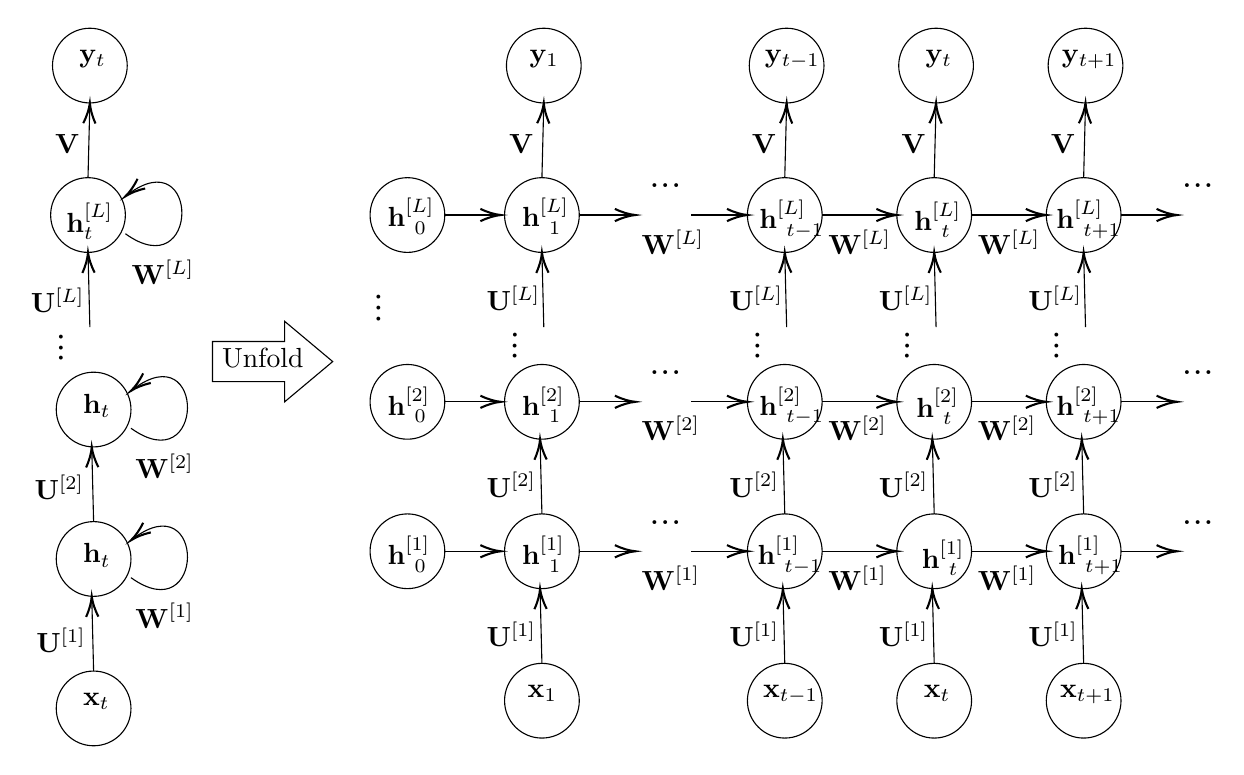
\begin{tikzpicture}[x=0.75pt,y=0.75pt,yscale=-0.9,xscale=0.9]
        %Shape: Ellipse [id:dp28408170140830746] 
        \draw   (24,35.87) .. controls (24,24.82) and (32.95,15.87) .. (44,15.87) .. controls (55.05,15.87) and (64,24.82) .. (64,35.87) .. controls (64,46.91) and (55.05,55.87) .. (44,55.87) .. controls (32.95,55.87) and (24,46.91) .. (24,35.87) -- cycle ;
        %Shape: Ellipse [id:dp8781268953519794] 
        \draw   (397,35.87) .. controls (397,24.82) and (405.95,15.87) .. (417,15.87) .. controls (428.05,15.87) and (437,24.82) .. (437,35.87) .. controls (437,46.91) and (428.05,55.87) .. (417,55.87) .. controls (405.95,55.87) and (397,46.91) .. (397,35.87) -- cycle ;
        %Shape: Ellipse [id:dp23070246888253831] 
        \draw   (557,35.87) .. controls (557,24.82) and (565.95,15.87) .. (577,15.87) .. controls (588.05,15.87) and (597,24.82) .. (597,35.87) .. controls (597,46.91) and (588.05,55.87) .. (577,55.87) .. controls (565.95,55.87) and (557,46.91) .. (557,35.87) -- cycle ;
        %Shape: Ellipse [id:dp8813319478015851] 
        \draw   (477,35.87) .. controls (477,24.82) and (485.95,15.87) .. (497,15.87) .. controls (508.05,15.87) and (517,24.82) .. (517,35.87) .. controls (517,46.91) and (508.05,55.87) .. (497,55.87) .. controls (485.95,55.87) and (477,46.91) .. (477,35.87) -- cycle ;
        %Shape: Ellipse [id:dp8173412138940122] 
        \draw   (267,35.87) .. controls (267,24.82) and (275.95,15.87) .. (287,15.87) .. controls (298.05,15.87) and (307,24.82) .. (307,35.87) .. controls (307,46.91) and (298.05,55.87) .. (287,55.87) .. controls (275.95,55.87) and (267,46.91) .. (267,35.87) -- cycle ;
        %Curve Lines [id:da5852340038150265] 
        \draw [color={rgb, 255:red, 0; green, 0; blue, 0 }  ,draw opacity=1 ]   (63,125.87) .. controls (102.93,154.58) and (103.33,75.48) .. (64.2,104.94) ;
        \draw [shift={(63,105.87)}, rotate = 321.57] [color={rgb, 255:red, 0; green, 0; blue, 0 }  ,draw opacity=1 ][line width=0.75]    (10.93,-3.29) .. controls (6.95,-1.4) and (3.31,-0.3) .. (0,0) .. controls (3.31,0.3) and (6.95,1.4) .. (10.93,3.29)   ;
        %Right Arrow [id:dp9792060545910206] 
        \draw   (109.66,183.55) -- (148.27,183.55) -- (148.27,172.77) -- (174,194.32) -- (148.27,215.87) -- (148.27,205.09) -- (109.66,205.09) -- cycle ;
        %Straight Lines [id:da04658286485976837] 
        \draw [color={rgb, 255:red, 0; green, 0; blue, 0 }  ,draw opacity=1 ]   (286,95.87) -- (286.95,57.87) ;
        \draw [shift={(287,55.87)}, rotate = 91.43] [color={rgb, 255:red, 0; green, 0; blue, 0 }  ,draw opacity=1 ][line width=0.75]    (10.93,-3.29) .. controls (6.95,-1.4) and (3.31,-0.3) .. (0,0) .. controls (3.31,0.3) and (6.95,1.4) .. (10.93,3.29)   ;
        %Shape: Ellipse [id:dp6328894287664162] 
        \draw   (23,115.87) .. controls (23,104.82) and (31.95,95.87) .. (43,95.87) .. controls (54.05,95.87) and (63,104.82) .. (63,115.87) .. controls (63,126.91) and (54.05,135.87) .. (43,135.87) .. controls (31.95,135.87) and (23,126.91) .. (23,115.87) -- cycle ;
        %Shape: Ellipse [id:dp25191747098174755] 
        \draw   (396,115.87) .. controls (396,104.82) and (404.95,95.87) .. (416,95.87) .. controls (427.05,95.87) and (436,104.82) .. (436,115.87) .. controls (436,126.91) and (427.05,135.87) .. (416,135.87) .. controls (404.95,135.87) and (396,126.91) .. (396,115.87) -- cycle ;
        %Shape: Ellipse [id:dp006489502181648232] 
        \draw   (556,115.87) .. controls (556,104.82) and (564.95,95.87) .. (576,95.87) .. controls (587.05,95.87) and (596,104.82) .. (596,115.87) .. controls (596,126.91) and (587.05,135.87) .. (576,135.87) .. controls (564.95,135.87) and (556,126.91) .. (556,115.87) -- cycle ;
        %Shape: Ellipse [id:dp17867093366227582] 
        \draw   (476,115.87) .. controls (476,104.82) and (484.95,95.87) .. (496,95.87) .. controls (507.05,95.87) and (516,104.82) .. (516,115.87) .. controls (516,126.91) and (507.05,135.87) .. (496,135.87) .. controls (484.95,135.87) and (476,126.91) .. (476,115.87) -- cycle ;
        %Shape: Ellipse [id:dp6982181811077917] 
        \draw   (266,115.87) .. controls (266,104.82) and (274.95,95.87) .. (286,95.87) .. controls (297.05,95.87) and (306,104.82) .. (306,115.87) .. controls (306,126.91) and (297.05,135.87) .. (286,135.87) .. controls (274.95,135.87) and (266,126.91) .. (266,115.87) -- cycle ;
        %Straight Lines [id:da48136805194677024] 
        \draw [color={rgb, 255:red, 0; green, 0; blue, 0 }  ,draw opacity=1 ]   (306,115.87) -- (334,115.87) ;
        \draw [shift={(336,115.87)}, rotate = 180] [color={rgb, 255:red, 0; green, 0; blue, 0 }  ,draw opacity=1 ][line width=0.75]    (10.93,-3.29) .. controls (6.95,-1.4) and (3.31,-0.3) .. (0,0) .. controls (3.31,0.3) and (6.95,1.4) .. (10.93,3.29)   ;
        %Straight Lines [id:da7629973938877173] 
        \draw [color={rgb, 255:red, 0; green, 0; blue, 0 }  ,draw opacity=1 ]   (366,115.87) -- (394,115.87) ;
        \draw [shift={(396,115.87)}, rotate = 180] [color={rgb, 255:red, 0; green, 0; blue, 0 }  ,draw opacity=1 ][line width=0.75]    (10.93,-3.29) .. controls (6.95,-1.4) and (3.31,-0.3) .. (0,0) .. controls (3.31,0.3) and (6.95,1.4) .. (10.93,3.29)   ;
        %Straight Lines [id:da48946711660534215] 
        \draw [color={rgb, 255:red, 0; green, 0; blue, 0 }  ,draw opacity=1 ]   (436,115.87) -- (474,115.87) ;
        \draw [shift={(476,115.87)}, rotate = 180] [color={rgb, 255:red, 0; green, 0; blue, 0 }  ,draw opacity=1 ][line width=0.75]    (10.93,-3.29) .. controls (6.95,-1.4) and (3.31,-0.3) .. (0,0) .. controls (3.31,0.3) and (6.95,1.4) .. (10.93,3.29)   ;
        %Straight Lines [id:da25906109638156805] 
        \draw [color={rgb, 255:red, 0; green, 0; blue, 0 }  ,draw opacity=1 ]   (516,115.87) -- (554,115.87) ;
        \draw [shift={(556,115.87)}, rotate = 180] [color={rgb, 255:red, 0; green, 0; blue, 0 }  ,draw opacity=1 ][line width=0.75]    (10.93,-3.29) .. controls (6.95,-1.4) and (3.31,-0.3) .. (0,0) .. controls (3.31,0.3) and (6.95,1.4) .. (10.93,3.29)   ;
        %Straight Lines [id:da9188006912208824] 
        \draw [color={rgb, 255:red, 0; green, 0; blue, 0 }  ,draw opacity=1 ]   (596,115.87) -- (624,115.87) ;
        \draw [shift={(626,115.87)}, rotate = 180] [color={rgb, 255:red, 0; green, 0; blue, 0 }  ,draw opacity=1 ][line width=0.75]    (10.93,-3.29) .. controls (6.95,-1.4) and (3.31,-0.3) .. (0,0) .. controls (3.31,0.3) and (6.95,1.4) .. (10.93,3.29)   ;
        %Straight Lines [id:da8680491380322006] 
        \draw [color={rgb, 255:red, 0; green, 0; blue, 0 }  ,draw opacity=1 ]   (287,175.87) -- (286.05,137.87) ;
        \draw [shift={(286,135.87)}, rotate = 88.57] [color={rgb, 255:red, 0; green, 0; blue, 0 }  ,draw opacity=1 ][line width=0.75]    (10.93,-3.29) .. controls (6.95,-1.4) and (3.31,-0.3) .. (0,0) .. controls (3.31,0.3) and (6.95,1.4) .. (10.93,3.29)   ;
        %Straight Lines [id:da7400484354415602] 
        \draw [color={rgb, 255:red, 0; green, 0; blue, 0 }  ,draw opacity=1 ]   (416,95.87) -- (416.95,57.87) ;
        \draw [shift={(417,55.87)}, rotate = 91.43] [color={rgb, 255:red, 0; green, 0; blue, 0 }  ,draw opacity=1 ][line width=0.75]    (10.93,-3.29) .. controls (6.95,-1.4) and (3.31,-0.3) .. (0,0) .. controls (3.31,0.3) and (6.95,1.4) .. (10.93,3.29)   ;
        %Straight Lines [id:da1345438068872269] 
        \draw [color={rgb, 255:red, 0; green, 0; blue, 0 }  ,draw opacity=1 ]   (417,175.87) -- (416.05,137.87) ;
        \draw [shift={(416,135.87)}, rotate = 88.57] [color={rgb, 255:red, 0; green, 0; blue, 0 }  ,draw opacity=1 ][line width=0.75]    (10.93,-3.29) .. controls (6.95,-1.4) and (3.31,-0.3) .. (0,0) .. controls (3.31,0.3) and (6.95,1.4) .. (10.93,3.29)   ;
        %Straight Lines [id:da6433457414107624] 
        \draw [color={rgb, 255:red, 0; green, 0; blue, 0 }  ,draw opacity=1 ]   (496,95.87) -- (496.95,57.87) ;
        \draw [shift={(497,55.87)}, rotate = 91.43] [color={rgb, 255:red, 0; green, 0; blue, 0 }  ,draw opacity=1 ][line width=0.75]    (10.93,-3.29) .. controls (6.95,-1.4) and (3.31,-0.3) .. (0,0) .. controls (3.31,0.3) and (6.95,1.4) .. (10.93,3.29)   ;
        %Straight Lines [id:da7669273924950717] 
        \draw [color={rgb, 255:red, 0; green, 0; blue, 0 }  ,draw opacity=1 ]   (497,175.87) -- (496.05,137.87) ;
        \draw [shift={(496,135.87)}, rotate = 88.57] [color={rgb, 255:red, 0; green, 0; blue, 0 }  ,draw opacity=1 ][line width=0.75]    (10.93,-3.29) .. controls (6.95,-1.4) and (3.31,-0.3) .. (0,0) .. controls (3.31,0.3) and (6.95,1.4) .. (10.93,3.29)   ;
        %Straight Lines [id:da5719741520220034] 
        \draw [color={rgb, 255:red, 0; green, 0; blue, 0 }  ,draw opacity=1 ]   (576,95.87) -- (576.95,57.87) ;
        \draw [shift={(577,55.87)}, rotate = 91.43] [color={rgb, 255:red, 0; green, 0; blue, 0 }  ,draw opacity=1 ][line width=0.75]    (10.93,-3.29) .. controls (6.95,-1.4) and (3.31,-0.3) .. (0,0) .. controls (3.31,0.3) and (6.95,1.4) .. (10.93,3.29)   ;
        %Straight Lines [id:da12398139085538262] 
        \draw [color={rgb, 255:red, 0; green, 0; blue, 0 }  ,draw opacity=1 ]   (577,175.87) -- (576.05,137.87) ;
        \draw [shift={(576,135.87)}, rotate = 88.57] [color={rgb, 255:red, 0; green, 0; blue, 0 }  ,draw opacity=1 ][line width=0.75]    (10.93,-3.29) .. controls (6.95,-1.4) and (3.31,-0.3) .. (0,0) .. controls (3.31,0.3) and (6.95,1.4) .. (10.93,3.29)   ;
        %Straight Lines [id:da2531008483395709] 
        \draw [color={rgb, 255:red, 0; green, 0; blue, 0 }  ,draw opacity=1 ]   (43,95.87) -- (43.95,57.87) ;
        \draw [shift={(44,55.87)}, rotate = 91.43] [color={rgb, 255:red, 0; green, 0; blue, 0 }  ,draw opacity=1 ][line width=0.75]    (10.93,-3.29) .. controls (6.95,-1.4) and (3.31,-0.3) .. (0,0) .. controls (3.31,0.3) and (6.95,1.4) .. (10.93,3.29)   ;
        %Straight Lines [id:da3139176439341236] 
        \draw [color={rgb, 255:red, 0; green, 0; blue, 0 }  ,draw opacity=1 ]   (44,175.87) -- (43.05,137.87) ;
        \draw [shift={(43,135.87)}, rotate = 88.57] [color={rgb, 255:red, 0; green, 0; blue, 0 }  ,draw opacity=1 ][line width=0.75]    (10.93,-3.29) .. controls (6.95,-1.4) and (3.31,-0.3) .. (0,0) .. controls (3.31,0.3) and (6.95,1.4) .. (10.93,3.29)   ;
        %Shape: Ellipse [id:dp667428376192245] 
        \draw   (26,380) .. controls (26,368.95) and (34.95,360) .. (46,360) .. controls (57.05,360) and (66,368.95) .. (66,380) .. controls (66,391.05) and (57.05,400) .. (46,400) .. controls (34.95,400) and (26,391.05) .. (26,380) -- cycle ;
        %Shape: Ellipse [id:dp3516553987469757] 
        \draw   (396,375.87) .. controls (396,364.82) and (404.95,355.87) .. (416,355.87) .. controls (427.05,355.87) and (436,364.82) .. (436,375.87) .. controls (436,386.91) and (427.05,395.87) .. (416,395.87) .. controls (404.95,395.87) and (396,386.91) .. (396,375.87) -- cycle ;
        %Shape: Ellipse [id:dp6472435395321006] 
        \draw   (556,375.87) .. controls (556,364.82) and (564.95,355.87) .. (576,355.87) .. controls (587.05,355.87) and (596,364.82) .. (596,375.87) .. controls (596,386.91) and (587.05,395.87) .. (576,395.87) .. controls (564.95,395.87) and (556,386.91) .. (556,375.87) -- cycle ;
        %Shape: Ellipse [id:dp777227070793655] 
        \draw   (476,375.87) .. controls (476,364.82) and (484.95,355.87) .. (496,355.87) .. controls (507.05,355.87) and (516,364.82) .. (516,375.87) .. controls (516,386.91) and (507.05,395.87) .. (496,395.87) .. controls (484.95,395.87) and (476,386.91) .. (476,375.87) -- cycle ;
        %Shape: Ellipse [id:dp24727587216480584] 
        \draw   (266,375.87) .. controls (266,364.82) and (274.95,355.87) .. (286,355.87) .. controls (297.05,355.87) and (306,364.82) .. (306,375.87) .. controls (306,386.91) and (297.05,395.87) .. (286,395.87) .. controls (274.95,395.87) and (266,386.91) .. (266,375.87) -- cycle ;
        %Straight Lines [id:da6480383110766228] 
        \draw [color={rgb, 255:red, 0; green, 0; blue, 0 }  ,draw opacity=1 ]   (286,355.87) -- (285.05,317.87) ;
        \draw [shift={(285,315.87)}, rotate = 88.57] [color={rgb, 255:red, 0; green, 0; blue, 0 }  ,draw opacity=1 ][line width=0.75]    (10.93,-3.29) .. controls (6.95,-1.4) and (3.31,-0.3) .. (0,0) .. controls (3.31,0.3) and (6.95,1.4) .. (10.93,3.29)   ;
        %Straight Lines [id:da3234423140056528] 
        \draw [color={rgb, 255:red, 0; green, 0; blue, 0 }  ,draw opacity=1 ]   (416,355.87) -- (415.05,317.87) ;
        \draw [shift={(415,315.87)}, rotate = 88.57] [color={rgb, 255:red, 0; green, 0; blue, 0 }  ,draw opacity=1 ][line width=0.75]    (10.93,-3.29) .. controls (6.95,-1.4) and (3.31,-0.3) .. (0,0) .. controls (3.31,0.3) and (6.95,1.4) .. (10.93,3.29)   ;
        %Straight Lines [id:da3097428942055547] 
        \draw [color={rgb, 255:red, 0; green, 0; blue, 0 }  ,draw opacity=1 ]   (496,355.87) -- (495.05,317.87) ;
        \draw [shift={(495,315.87)}, rotate = 88.57] [color={rgb, 255:red, 0; green, 0; blue, 0 }  ,draw opacity=1 ][line width=0.75]    (10.93,-3.29) .. controls (6.95,-1.4) and (3.31,-0.3) .. (0,0) .. controls (3.31,0.3) and (6.95,1.4) .. (10.93,3.29)   ;
        %Straight Lines [id:da4628558661714015] 
        \draw [color={rgb, 255:red, 0; green, 0; blue, 0 }  ,draw opacity=1 ]   (576,355.87) -- (575.05,317.87) ;
        \draw [shift={(575,315.87)}, rotate = 88.57] [color={rgb, 255:red, 0; green, 0; blue, 0 }  ,draw opacity=1 ][line width=0.75]    (10.93,-3.29) .. controls (6.95,-1.4) and (3.31,-0.3) .. (0,0) .. controls (3.31,0.3) and (6.95,1.4) .. (10.93,3.29)   ;
        %Straight Lines [id:da5014238028882425] 
        \draw [color={rgb, 255:red, 0; green, 0; blue, 0 }  ,draw opacity=1 ]   (46,360) -- (45.05,322) ;
        \draw [shift={(45,320)}, rotate = 88.57] [color={rgb, 255:red, 0; green, 0; blue, 0 }  ,draw opacity=1 ][line width=0.75]    (10.93,-3.29) .. controls (6.95,-1.4) and (3.31,-0.3) .. (0,0) .. controls (3.31,0.3) and (6.95,1.4) .. (10.93,3.29)   ;
        %Curve Lines [id:da0038695441555764987] 
        \draw [color={rgb, 255:red, 0; green, 0; blue, 0 }  ,draw opacity=1 ]   (66,310) .. controls (105.93,338.71) and (106.33,259.61) .. (67.2,289.07) ;
        \draw [shift={(66,290)}, rotate = 321.57] [color={rgb, 255:red, 0; green, 0; blue, 0 }  ,draw opacity=1 ][line width=0.75]    (10.93,-3.29) .. controls (6.95,-1.4) and (3.31,-0.3) .. (0,0) .. controls (3.31,0.3) and (6.95,1.4) .. (10.93,3.29)   ;
        %Shape: Ellipse [id:dp6090800570288175] 
        \draw   (26,300) .. controls (26,288.95) and (34.95,280) .. (46,280) .. controls (57.05,280) and (66,288.95) .. (66,300) .. controls (66,311.05) and (57.05,320) .. (46,320) .. controls (34.95,320) and (26,311.05) .. (26,300) -- cycle ;
        %Shape: Ellipse [id:dp814692294048333] 
        \draw   (396,295.87) .. controls (396,284.82) and (404.95,275.87) .. (416,275.87) .. controls (427.05,275.87) and (436,284.82) .. (436,295.87) .. controls (436,306.91) and (427.05,315.87) .. (416,315.87) .. controls (404.95,315.87) and (396,306.91) .. (396,295.87) -- cycle ;
        %Shape: Ellipse [id:dp7431446264337986] 
        \draw   (556,295.87) .. controls (556,284.82) and (564.95,275.87) .. (576,275.87) .. controls (587.05,275.87) and (596,284.82) .. (596,295.87) .. controls (596,306.91) and (587.05,315.87) .. (576,315.87) .. controls (564.95,315.87) and (556,306.91) .. (556,295.87) -- cycle ;
        %Shape: Ellipse [id:dp3134154372580471] 
        \draw   (476,295.87) .. controls (476,284.82) and (484.95,275.87) .. (496,275.87) .. controls (507.05,275.87) and (516,284.82) .. (516,295.87) .. controls (516,306.91) and (507.05,315.87) .. (496,315.87) .. controls (484.95,315.87) and (476,306.91) .. (476,295.87) -- cycle ;
        %Shape: Ellipse [id:dp9974427304065943] 
        \draw   (266,295.87) .. controls (266,284.82) and (274.95,275.87) .. (286,275.87) .. controls (297.05,275.87) and (306,284.82) .. (306,295.87) .. controls (306,306.91) and (297.05,315.87) .. (286,315.87) .. controls (274.95,315.87) and (266,306.91) .. (266,295.87) -- cycle ;
        %Straight Lines [id:da6122510674754102] 
        \draw [color={rgb, 255:red, 0; green, 0; blue, 0 }  ,draw opacity=1 ]   (306,295.87) -- (334,295.87) ;
        \draw [shift={(336,295.87)}, rotate = 180] [color={rgb, 255:red, 0; green, 0; blue, 0 }  ,draw opacity=1 ][line width=0.75]    (10.93,-3.29) .. controls (6.95,-1.4) and (3.31,-0.3) .. (0,0) .. controls (3.31,0.3) and (6.95,1.4) .. (10.93,3.29)   ;
        %Straight Lines [id:da8762576001287141] 
        \draw [color={rgb, 255:red, 0; green, 0; blue, 0 }  ,draw opacity=1 ]   (366,295.87) -- (394,295.87) ;
        \draw [shift={(396,295.87)}, rotate = 180] [color={rgb, 255:red, 0; green, 0; blue, 0 }  ,draw opacity=1 ][line width=0.75]    (10.93,-3.29) .. controls (6.95,-1.4) and (3.31,-0.3) .. (0,0) .. controls (3.31,0.3) and (6.95,1.4) .. (10.93,3.29)   ;
        %Straight Lines [id:da19417361046991521] 
        \draw [color={rgb, 255:red, 0; green, 0; blue, 0 }  ,draw opacity=1 ]   (436,295.87) -- (474,295.87) ;
        \draw [shift={(476,295.87)}, rotate = 180] [color={rgb, 255:red, 0; green, 0; blue, 0 }  ,draw opacity=1 ][line width=0.75]    (10.93,-3.29) .. controls (6.95,-1.4) and (3.31,-0.3) .. (0,0) .. controls (3.31,0.3) and (6.95,1.4) .. (10.93,3.29)   ;
        %Straight Lines [id:da48160692056586774] 
        \draw [color={rgb, 255:red, 0; green, 0; blue, 0 }  ,draw opacity=1 ]   (516,295.87) -- (554,295.87) ;
        \draw [shift={(556,295.87)}, rotate = 180] [color={rgb, 255:red, 0; green, 0; blue, 0 }  ,draw opacity=1 ][line width=0.75]    (10.93,-3.29) .. controls (6.95,-1.4) and (3.31,-0.3) .. (0,0) .. controls (3.31,0.3) and (6.95,1.4) .. (10.93,3.29)   ;
        %Straight Lines [id:da44061532346635235] 
        \draw [color={rgb, 255:red, 0; green, 0; blue, 0 }  ,draw opacity=1 ]   (596,295.87) -- (624,295.87) ;
        \draw [shift={(626,295.87)}, rotate = 180] [color={rgb, 255:red, 0; green, 0; blue, 0 }  ,draw opacity=1 ][line width=0.75]    (10.93,-3.29) .. controls (6.95,-1.4) and (3.31,-0.3) .. (0,0) .. controls (3.31,0.3) and (6.95,1.4) .. (10.93,3.29)   ;
        %Straight Lines [id:da7735315393550828] 
        \draw [color={rgb, 255:red, 0; green, 0; blue, 0 }  ,draw opacity=1 ]   (286,275.87) -- (285.05,237.87) ;
        \draw [shift={(285,235.87)}, rotate = 88.57] [color={rgb, 255:red, 0; green, 0; blue, 0 }  ,draw opacity=1 ][line width=0.75]    (10.93,-3.29) .. controls (6.95,-1.4) and (3.31,-0.3) .. (0,0) .. controls (3.31,0.3) and (6.95,1.4) .. (10.93,3.29)   ;
        %Straight Lines [id:da31248700265465956] 
        \draw [color={rgb, 255:red, 0; green, 0; blue, 0 }  ,draw opacity=1 ]   (416,275.87) -- (415.05,237.87) ;
        \draw [shift={(415,235.87)}, rotate = 88.57] [color={rgb, 255:red, 0; green, 0; blue, 0 }  ,draw opacity=1 ][line width=0.75]    (10.93,-3.29) .. controls (6.95,-1.4) and (3.31,-0.3) .. (0,0) .. controls (3.31,0.3) and (6.95,1.4) .. (10.93,3.29)   ;
        %Straight Lines [id:da22979184387608442] 
        \draw [color={rgb, 255:red, 0; green, 0; blue, 0 }  ,draw opacity=1 ]   (496,275.87) -- (495.05,237.87) ;
        \draw [shift={(495,235.87)}, rotate = 88.57] [color={rgb, 255:red, 0; green, 0; blue, 0 }  ,draw opacity=1 ][line width=0.75]    (10.93,-3.29) .. controls (6.95,-1.4) and (3.31,-0.3) .. (0,0) .. controls (3.31,0.3) and (6.95,1.4) .. (10.93,3.29)   ;
        %Straight Lines [id:da6868203706104177] 
        \draw [color={rgb, 255:red, 0; green, 0; blue, 0 }  ,draw opacity=1 ]   (576,275.87) -- (575.05,237.87) ;
        \draw [shift={(575,235.87)}, rotate = 88.57] [color={rgb, 255:red, 0; green, 0; blue, 0 }  ,draw opacity=1 ][line width=0.75]    (10.93,-3.29) .. controls (6.95,-1.4) and (3.31,-0.3) .. (0,0) .. controls (3.31,0.3) and (6.95,1.4) .. (10.93,3.29)   ;
        %Straight Lines [id:da7914857117545093] 
        \draw [color={rgb, 255:red, 0; green, 0; blue, 0 }  ,draw opacity=1 ]   (46,280) -- (45.05,242) ;
        \draw [shift={(45,240)}, rotate = 88.57] [color={rgb, 255:red, 0; green, 0; blue, 0 }  ,draw opacity=1 ][line width=0.75]    (10.93,-3.29) .. controls (6.95,-1.4) and (3.31,-0.3) .. (0,0) .. controls (3.31,0.3) and (6.95,1.4) .. (10.93,3.29)   ;
        %Curve Lines [id:da17078665595389708] 
        \draw [color={rgb, 255:red, 0; green, 0; blue, 0 }  ,draw opacity=1 ]   (66,230) .. controls (105.93,258.71) and (106.33,179.61) .. (67.2,209.07) ;
        \draw [shift={(66,210)}, rotate = 321.57] [color={rgb, 255:red, 0; green, 0; blue, 0 }  ,draw opacity=1 ][line width=0.75]    (10.93,-3.29) .. controls (6.95,-1.4) and (3.31,-0.3) .. (0,0) .. controls (3.31,0.3) and (6.95,1.4) .. (10.93,3.29)   ;
        %Shape: Ellipse [id:dp942876704165063] 
        \draw   (26,220) .. controls (26,208.95) and (34.95,200) .. (46,200) .. controls (57.05,200) and (66,208.95) .. (66,220) .. controls (66,231.05) and (57.05,240) .. (46,240) .. controls (34.95,240) and (26,231.05) .. (26,220) -- cycle ;
        %Shape: Ellipse [id:dp6726841288284007] 
        \draw   (396,215.87) .. controls (396,204.82) and (404.95,195.87) .. (416,195.87) .. controls (427.05,195.87) and (436,204.82) .. (436,215.87) .. controls (436,226.91) and (427.05,235.87) .. (416,235.87) .. controls (404.95,235.87) and (396,226.91) .. (396,215.87) -- cycle ;
        %Shape: Ellipse [id:dp26675511576359034] 
        \draw   (556,215.87) .. controls (556,204.82) and (564.95,195.87) .. (576,195.87) .. controls (587.05,195.87) and (596,204.82) .. (596,215.87) .. controls (596,226.91) and (587.05,235.87) .. (576,235.87) .. controls (564.95,235.87) and (556,226.91) .. (556,215.87) -- cycle ;
        %Shape: Ellipse [id:dp015707245318489216] 
        \draw   (476,215.87) .. controls (476,204.82) and (484.95,195.87) .. (496,195.87) .. controls (507.05,195.87) and (516,204.82) .. (516,215.87) .. controls (516,226.91) and (507.05,235.87) .. (496,235.87) .. controls (484.95,235.87) and (476,226.91) .. (476,215.87) -- cycle ;
        %Shape: Ellipse [id:dp7345225793669115] 
        \draw   (266,215.87) .. controls (266,204.82) and (274.95,195.87) .. (286,195.87) .. controls (297.05,195.87) and (306,204.82) .. (306,215.87) .. controls (306,226.91) and (297.05,235.87) .. (286,235.87) .. controls (274.95,235.87) and (266,226.91) .. (266,215.87) -- cycle ;
        %Straight Lines [id:da6699501367062208] 
        \draw [color={rgb, 255:red, 0; green, 0; blue, 0 }  ,draw opacity=1 ]   (306,215.87) -- (334,215.87) ;
        \draw [shift={(336,215.87)}, rotate = 180] [color={rgb, 255:red, 0; green, 0; blue, 0 }  ,draw opacity=1 ][line width=0.75]    (10.93,-3.29) .. controls (6.95,-1.4) and (3.31,-0.3) .. (0,0) .. controls (3.31,0.3) and (6.95,1.4) .. (10.93,3.29)   ;
        %Straight Lines [id:da5370938326059405] 
        \draw [color={rgb, 255:red, 0; green, 0; blue, 0 }  ,draw opacity=1 ]   (366,215.87) -- (394,215.87) ;
        \draw [shift={(396,215.87)}, rotate = 180] [color={rgb, 255:red, 0; green, 0; blue, 0 }  ,draw opacity=1 ][line width=0.75]    (10.93,-3.29) .. controls (6.95,-1.4) and (3.31,-0.3) .. (0,0) .. controls (3.31,0.3) and (6.95,1.4) .. (10.93,3.29)   ;
        %Straight Lines [id:da7734328391970957] 
        \draw [color={rgb, 255:red, 0; green, 0; blue, 0 }  ,draw opacity=1 ]   (436,215.87) -- (474,215.87) ;
        \draw [shift={(476,215.87)}, rotate = 180] [color={rgb, 255:red, 0; green, 0; blue, 0 }  ,draw opacity=1 ][line width=0.75]    (10.93,-3.29) .. controls (6.95,-1.4) and (3.31,-0.3) .. (0,0) .. controls (3.31,0.3) and (6.95,1.4) .. (10.93,3.29)   ;
        %Straight Lines [id:da09004561395765753] 
        \draw [color={rgb, 255:red, 0; green, 0; blue, 0 }  ,draw opacity=1 ]   (516,215.87) -- (554,215.87) ;
        \draw [shift={(556,215.87)}, rotate = 180] [color={rgb, 255:red, 0; green, 0; blue, 0 }  ,draw opacity=1 ][line width=0.75]    (10.93,-3.29) .. controls (6.95,-1.4) and (3.31,-0.3) .. (0,0) .. controls (3.31,0.3) and (6.95,1.4) .. (10.93,3.29)   ;
        %Straight Lines [id:da06318399443660994] 
        \draw [color={rgb, 255:red, 0; green, 0; blue, 0 }  ,draw opacity=1 ]   (596,215.87) -- (624,215.87) ;
        \draw [shift={(626,215.87)}, rotate = 180] [color={rgb, 255:red, 0; green, 0; blue, 0 }  ,draw opacity=1 ][line width=0.75]    (10.93,-3.29) .. controls (6.95,-1.4) and (3.31,-0.3) .. (0,0) .. controls (3.31,0.3) and (6.95,1.4) .. (10.93,3.29)   ;
        %Shape: Ellipse [id:dp007975160952559124] 
        \draw   (194,115.87) .. controls (194,104.82) and (202.95,95.87) .. (214,95.87) .. controls (225.05,95.87) and (234,104.82) .. (234,115.87) .. controls (234,126.91) and (225.05,135.87) .. (214,135.87) .. controls (202.95,135.87) and (194,126.91) .. (194,115.87) -- cycle ;
        %Straight Lines [id:da06838614506463814] 
        \draw [color={rgb, 255:red, 0; green, 0; blue, 0 }  ,draw opacity=1 ]   (234,115.87) -- (262,115.87) ;
        \draw [shift={(264,115.87)}, rotate = 180] [color={rgb, 255:red, 0; green, 0; blue, 0 }  ,draw opacity=1 ][line width=0.75]    (10.93,-3.29) .. controls (6.95,-1.4) and (3.31,-0.3) .. (0,0) .. controls (3.31,0.3) and (6.95,1.4) .. (10.93,3.29)   ;
        %Shape: Ellipse [id:dp8070512895277284] 
        \draw   (194,215.87) .. controls (194,204.82) and (202.95,195.87) .. (214,195.87) .. controls (225.05,195.87) and (234,204.82) .. (234,215.87) .. controls (234,226.91) and (225.05,235.87) .. (214,235.87) .. controls (202.95,235.87) and (194,226.91) .. (194,215.87) -- cycle ;
        %Straight Lines [id:da8695420479992435] 
        \draw [color={rgb, 255:red, 0; green, 0; blue, 0 }  ,draw opacity=1 ]   (234,215.87) -- (262,215.87) ;
        \draw [shift={(264,215.87)}, rotate = 180] [color={rgb, 255:red, 0; green, 0; blue, 0 }  ,draw opacity=1 ][line width=0.75]    (10.93,-3.29) .. controls (6.95,-1.4) and (3.31,-0.3) .. (0,0) .. controls (3.31,0.3) and (6.95,1.4) .. (10.93,3.29)   ;
        %Shape: Ellipse [id:dp37022230422863234] 
        \draw   (194,295.87) .. controls (194,284.82) and (202.95,275.87) .. (214,275.87) .. controls (225.05,275.87) and (234,284.82) .. (234,295.87) .. controls (234,306.91) and (225.05,315.87) .. (214,315.87) .. controls (202.95,315.87) and (194,306.91) .. (194,295.87) -- cycle ;
        %Straight Lines [id:da018050318834118118] 
        \draw [color={rgb, 255:red, 0; green, 0; blue, 0 }  ,draw opacity=1 ]   (234,295.87) -- (262,295.87) ;
        \draw [shift={(264,295.87)}, rotate = 180] [color={rgb, 255:red, 0; green, 0; blue, 0 }  ,draw opacity=1 ][line width=0.75]    (10.93,-3.29) .. controls (6.95,-1.4) and (3.31,-0.3) .. (0,0) .. controls (3.31,0.3) and (6.95,1.4) .. (10.93,3.29)   ;

        % Text Node
        \draw (342,97.87) node [anchor=north west][inner sep=0.75pt]  [font=\Large] [align=left] {...};
        % Text Node
        \draw (278,26.27) node [anchor=north west][inner sep=0.75pt]  [font=\normalsize]  {$\mathbf{y}_{1}$};
        % Text Node
        \draw (404,26.27) node [anchor=north west][inner sep=0.75pt]  [font=\normalsize]  {$\mathbf{y}_{t-1}$};
        % Text Node
        \draw (113.36,185.86) node [anchor=north west][inner sep=0.75pt]   [align=left] {Unfold};
        % Text Node
        \draw (338,122.27) node [anchor=north west][inner sep=0.75pt]  [font=\normalsize,color={rgb, 255:red, 0; green, 0; blue, 0 }  ,opacity=1 ]  {$\mathbf{W}^{[ L]}$};
        % Text Node
        \draw (490,26.27) node [anchor=north west][inner sep=0.75pt]  [font=\normalsize]  {$\mathbf{y}_{t}$};
        % Text Node
        \draw (563,26.27) node [anchor=north west][inner sep=0.75pt]  [font=\normalsize]  {$\mathbf{y}_{t+1}$};
        % Text Node
        \draw (37,26.27) node [anchor=north west][inner sep=0.75pt]  [font=\normalsize]  {$\mathbf{y}_{t}$};
        % Text Node
        \draw (267,71.27) node [anchor=north west][inner sep=0.75pt]  [font=\normalsize,color={rgb, 255:red, 0; green, 0; blue, 0 }  ,opacity=1 ]  {$\mathbf{V}$};
        % Text Node
        \draw (274,105.27) node [anchor=north west][inner sep=0.75pt]  [font=\normalsize]  {$\mathbf{h}_{\ 1}^{[ L]}$};
        % Text Node
        \draw (401,106.27) node [anchor=north west][inner sep=0.75pt]  [font=\normalsize]  {$\mathbf{h}_{\ t-1}^{[ L]}$};
        % Text Node
        \draw (484,107.27) node [anchor=north west][inner sep=0.75pt]  [font=\normalsize]  {$\mathbf{h}_{\ t}^{[ L]}$};
        % Text Node
        \draw (560,106.27) node [anchor=north west][inner sep=0.75pt]  [font=\normalsize]  {$\mathbf{h}_{\ t+1}^{[ L]}$};
        % Text Node
        \draw (627,97.87) node [anchor=north west][inner sep=0.75pt]  [font=\Large] [align=left] {...};
        % Text Node
        \draw (255,152.27) node [anchor=north west][inner sep=0.75pt]  [font=\normalsize,color={rgb, 255:red, 0; green, 0; blue, 0 }  ,opacity=1 ]  {$\mathbf{U}^{[ L]}$};
        % Text Node
        \draw (397,71.27) node [anchor=north west][inner sep=0.75pt]  [font=\normalsize,color={rgb, 255:red, 0; green, 0; blue, 0 }  ,opacity=1 ]  {$\mathbf{V}$};
        % Text Node
        \draw (477,71.27) node [anchor=north west][inner sep=0.75pt]  [font=\normalsize,color={rgb, 255:red, 0; green, 0; blue, 0 }  ,opacity=1 ]  {$\mathbf{V}$};
        % Text Node
        \draw (557,71.27) node [anchor=north west][inner sep=0.75pt]  [font=\normalsize,color={rgb, 255:red, 0; green, 0; blue, 0 }  ,opacity=1 ]  {$\mathbf{V}$};
        % Text Node
        \draw (24,71.27) node [anchor=north west][inner sep=0.75pt]  [font=\normalsize,color={rgb, 255:red, 0; green, 0; blue, 0 }  ,opacity=1 ]  {$\mathbf{V}$};
        % Text Node
        \draw (438,122.27) node [anchor=north west][inner sep=0.75pt]  [font=\normalsize,color={rgb, 255:red, 0; green, 0; blue, 0 }  ,opacity=1 ]  {$\mathbf{W}^{[ L]}$};
        % Text Node
        \draw (518,122.27) node [anchor=north west][inner sep=0.75pt]  [font=\normalsize,color={rgb, 255:red, 0; green, 0; blue, 0 }  ,opacity=1 ]  {$\mathbf{W}^{[ L]}$};
        % Text Node
        \draw (385,152.27) node [anchor=north west][inner sep=0.75pt]  [font=\normalsize,color={rgb, 255:red, 0; green, 0; blue, 0 }  ,opacity=1 ]  {$\mathbf{U}^{[ L]}$};
        % Text Node
        \draw (465,152.27) node [anchor=north west][inner sep=0.75pt]  [font=\normalsize,color={rgb, 255:red, 0; green, 0; blue, 0 }  ,opacity=1 ]  {$\mathbf{U}^{[ L]}$};
        % Text Node
        \draw (545,152.27) node [anchor=north west][inner sep=0.75pt]  [font=\normalsize,color={rgb, 255:red, 0; green, 0; blue, 0 }  ,opacity=1 ]  {$\mathbf{U}^{[ L]}$};
        % Text Node
        \draw (277,366.27) node [anchor=north west][inner sep=0.75pt]  [font=\normalsize]  {$\mathbf{x}_{1}$};
        % Text Node
        \draw (403,366.27) node [anchor=north west][inner sep=0.75pt]  [font=\normalsize]  {$\mathbf{x}_{t-1}$};
        % Text Node
        \draw (489,366.27) node [anchor=north west][inner sep=0.75pt]  [font=\normalsize]  {$\mathbf{x}_{t}$};
        % Text Node
        \draw (562,366.27) node [anchor=north west][inner sep=0.75pt]  [font=\normalsize]  {$\mathbf{x}_{t+1}$};
        % Text Node
        \draw (39,370.4) node [anchor=north west][inner sep=0.75pt]  [font=\normalsize]  {$\mathbf{x}_{t}$};
        % Text Node
        \draw (255,332.27) node [anchor=north west][inner sep=0.75pt]  [font=\normalsize,color={rgb, 255:red, 0; green, 0; blue, 0 }  ,opacity=1 ]  {$\mathbf{U}^{[ 1]}$};
        % Text Node
        \draw (385,332.27) node [anchor=north west][inner sep=0.75pt]  [font=\normalsize,color={rgb, 255:red, 0; green, 0; blue, 0 }  ,opacity=1 ]  {$\mathbf{U}^{[ 1]}$};
        % Text Node
        \draw (465,332.27) node [anchor=north west][inner sep=0.75pt]  [font=\normalsize,color={rgb, 255:red, 0; green, 0; blue, 0 }  ,opacity=1 ]  {$\mathbf{U}^{[ 1]}$};
        % Text Node
        \draw (545,332.27) node [anchor=north west][inner sep=0.75pt]  [font=\normalsize,color={rgb, 255:red, 0; green, 0; blue, 0 }  ,opacity=1 ]  {$\mathbf{U}^{[ 1]}$};
        % Text Node
        \draw (342,277.87) node [anchor=north west][inner sep=0.75pt]  [font=\Large] [align=left] {...};
        % Text Node
        \draw (338,302.27) node [anchor=north west][inner sep=0.75pt]  [font=\normalsize,color={rgb, 255:red, 0; green, 0; blue, 0 }  ,opacity=1 ]  {$\mathbf{W}^{[ 1]}$};
        % Text Node
        \draw (274,286.27) node [anchor=north west][inner sep=0.75pt]  [font=\normalsize]  {$\mathbf{h}_{\ 1}^{[ 1]}$};
        % Text Node
        \draw (400,286.27) node [anchor=north west][inner sep=0.75pt]  [font=\normalsize]  {$\mathbf{h}_{\ t-1}^{[ 1]}$};
        % Text Node
        \draw (488,288.27) node [anchor=north west][inner sep=0.75pt]  [font=\normalsize]  {$\mathbf{h}_{\ t}^{[ 1]}$};
        % Text Node
        \draw (561,286.27) node [anchor=north west][inner sep=0.75pt]  [font=\normalsize]  {$\mathbf{h}_{\ t+1}^{[ 1]}$};
        % Text Node
        \draw (39,290.4) node [anchor=north west][inner sep=0.75pt]  [font=\normalsize]  {$\mathbf{h}_{t}$};
        % Text Node
        \draw (627,277.87) node [anchor=north west][inner sep=0.75pt]  [font=\Large] [align=left] {...};
        % Text Node
        \draw (438,302.27) node [anchor=north west][inner sep=0.75pt]  [font=\normalsize,color={rgb, 255:red, 0; green, 0; blue, 0 }  ,opacity=1 ]  {$\mathbf{W}^{[ 1]}$};
        % Text Node
        \draw (518,302.27) node [anchor=north west][inner sep=0.75pt]  [font=\normalsize,color={rgb, 255:red, 0; green, 0; blue, 0 }  ,opacity=1 ]  {$\mathbf{W}^{[ 1]}$};
        % Text Node
        \draw (14,335.4) node [anchor=north west][inner sep=0.75pt]  [font=\normalsize,color={rgb, 255:red, 0; green, 0; blue, 0 }  ,opacity=1 ]  {$\mathbf{U}^{[ 1]}$};
        % Text Node
        \draw (67,322.4) node [anchor=north west][inner sep=0.75pt]  [font=\normalsize,color={rgb, 255:red, 0; green, 0; blue, 0 }  ,opacity=1 ]  {$\mathbf{W}^{[ 1]}$};
        % Text Node
        \draw (255,252.27) node [anchor=north west][inner sep=0.75pt]  [font=\normalsize,color={rgb, 255:red, 0; green, 0; blue, 0 }  ,opacity=1 ]  {$\mathbf{U}^{[ 2]}$};
        % Text Node
        \draw (385,252.27) node [anchor=north west][inner sep=0.75pt]  [font=\normalsize,color={rgb, 255:red, 0; green, 0; blue, 0 }  ,opacity=1 ]  {$\mathbf{U}^{[ 2]}$};
        % Text Node
        \draw (465,252.27) node [anchor=north west][inner sep=0.75pt]  [font=\normalsize,color={rgb, 255:red, 0; green, 0; blue, 0 }  ,opacity=1 ]  {$\mathbf{U}^{[ 2]}$};
        % Text Node
        \draw (545,252.27) node [anchor=north west][inner sep=0.75pt]  [font=\normalsize,color={rgb, 255:red, 0; green, 0; blue, 0 }  ,opacity=1 ]  {$\mathbf{U}^{[ 2]}$};
        % Text Node
        \draw (342,197.87) node [anchor=north west][inner sep=0.75pt]  [font=\Large] [align=left] {...};
        % Text Node
        \draw (338,222.27) node [anchor=north west][inner sep=0.75pt]  [font=\normalsize,color={rgb, 255:red, 0; green, 0; blue, 0 }  ,opacity=1 ]  {$\mathbf{W}^{[ 2]}$};
        % Text Node
        \draw (274,206.27) node [anchor=north west][inner sep=0.75pt]  [font=\normalsize]  {$\mathbf{h}_{\ 1}^{[ 2]}$};
        % Text Node
        \draw (401,206.27) node [anchor=north west][inner sep=0.75pt]  [font=\normalsize]  {$\mathbf{h}_{\ t-1}^{[ 2]}$};
        % Text Node
        \draw (485,207.27) node [anchor=north west][inner sep=0.75pt]  [font=\normalsize]  {$\mathbf{h}_{\ t}^{[ 2]}$};
        % Text Node
        \draw (560,206.27) node [anchor=north west][inner sep=0.75pt]  [font=\normalsize]  {$\mathbf{h}_{\ t+1}^{[ 2]}$};
        % Text Node
        \draw (39,210.4) node [anchor=north west][inner sep=0.75pt]  [font=\normalsize]  {$\mathbf{h}_{t}$};
        % Text Node
        \draw (627,197.87) node [anchor=north west][inner sep=0.75pt]  [font=\Large] [align=left] {...};
        % Text Node
        \draw (438,222.27) node [anchor=north west][inner sep=0.75pt]  [font=\normalsize,color={rgb, 255:red, 0; green, 0; blue, 0 }  ,opacity=1 ]  {$\mathbf{W}^{[ 2]}$};
        % Text Node
        \draw (518,222.27) node [anchor=north west][inner sep=0.75pt]  [font=\normalsize,color={rgb, 255:red, 0; green, 0; blue, 0 }  ,opacity=1 ]  {$\mathbf{W}^{[ 2]}$};
        % Text Node
        \draw (13,253.4) node [anchor=north west][inner sep=0.75pt]  [font=\normalsize,color={rgb, 255:red, 0; green, 0; blue, 0 }  ,opacity=1 ]  {$\mathbf{U}^{[ 2]}$};
        % Text Node
        \draw (67,242.4) node [anchor=north west][inner sep=0.75pt]  [font=\normalsize,color={rgb, 255:red, 0; green, 0; blue, 0 }  ,opacity=1 ]  {$\mathbf{W}^{[ 2]}$};
        % Text Node
        \draw (269,195.88) node [anchor=north west][inner sep=0.75pt]  [font=\Large,rotate=-270.25] [align=left] {...};
        % Text Node
        \draw (398.91,195.88) node [anchor=north west][inner sep=0.75pt]  [font=\Large,rotate=-270.25] [align=left] {...};
        % Text Node
        \draw (479,195.88) node [anchor=north west][inner sep=0.75pt]  [font=\Large,rotate=-270.25] [align=left] {...};
        % Text Node
        \draw (559,195.88) node [anchor=north west][inner sep=0.75pt]  [font=\Large,rotate=-270.25] [align=left] {...};
        % Text Node
        \draw (26,197.01) node [anchor=north west][inner sep=0.75pt]  [font=\Large,rotate=-270.25] [align=left] {...};
        % Text Node
        \draw (11,153.27) node [anchor=north west][inner sep=0.75pt]  [font=\normalsize,color={rgb, 255:red, 0; green, 0; blue, 0 }  ,opacity=1 ]  {$\mathbf{U}^{[ L]}$};
        % Text Node
        \draw (30,108.27) node [anchor=north west][inner sep=0.75pt]  [font=\normalsize]  {$\mathbf{h}_{t}^{[ L]}$};
        % Text Node
        \draw (65,138.27) node [anchor=north west][inner sep=0.75pt]  [font=\normalsize,color={rgb, 255:red, 0; green, 0; blue, 0 }  ,opacity=1 ]  {$\mathbf{W}^{[ L]}$};
        % Text Node
        \draw (202,105.27) node [anchor=north west][inner sep=0.75pt]  [font=\normalsize]  {$\mathbf{h}_{\ 0}^{[ L]}$};
        % Text Node
        \draw (202,206.27) node [anchor=north west][inner sep=0.75pt]  [font=\normalsize]  {$\mathbf{h}_{\ 0}^{[ 2]}$};
        % Text Node
        \draw (196,175.88) node [anchor=north west][inner sep=0.75pt]  [font=\Large,rotate=-270.25] [align=left] {...};
        % Text Node
        \draw (202,286.27) node [anchor=north west][inner sep=0.75pt]  [font=\normalsize]  {$\mathbf{h}_{\ 0}^{[ 1]}$};
      \end{tikzpicture}
      \caption{Stacked RNNs.} 
      \label{fig:stacked_rnn}
    \end{figure}

    Now in this case, there are more layers of hidden nodes that an input must go through before it reaches the output node. We can expand out the computations as such, for $t = 1, \ldots, \tau$, $l = 2, \ldots L$: 
    \begin{align}
      \mathbf{h}_t^{[1]} & = \boldsymbol{\sigma}_h \big( \mathbf{W}^{[1]} \mathbf{h}_{t-1}^{[1]} + \mathbf{U}^{[1]} \mathbf{x}_t + \mathbf{b}_h^{[1]} \big) \\
      \mathbf{h}_t^{[l]} & = \boldsymbol{\sigma}_h \big( \mathbf{W}^{[l]} \mathbf{h}_{t-1}^{[l]} + \mathbf{U}^{[l]} \mathbf{x}_t + \mathbf{b}_h^{[l]} \big) \\
      \mathbf{y}_t & = \boldsymbol{\sigma}_y \big( \mathbf{V} \mathbf{h}_t^{[L]} + \mathbf{b}_y^{[L]} \big) 
    \end{align}
    or we could get rid of the first equation all together if we set $\mathbf{x}_t = \mathbf{h}_t^{[0]}$. Note that the hidden nodes $\mathbf{h}^{[l]}_t$ for all $t$ and all $l \neq 0$ are all in $\mathbb{R}^h$, i.e. all hidden nodes will be $h$-dimensional. Therefore, most of the parameter matrices that we work with are square: $\mathbf{W}^{[l]} \in \mathbb{R}^{h \times h}$ and $\mathbf{U}^{[l]} \in \mathbb{R}^{h \times h}$ except for $\mathbf{U}^{[1]} \in \mathbb{R}^{h \times d}$. 

\subsection{Bidirectional RNNs}

  \subsubsection{PyTorch Implementation}

    The implementation in PyTorch actually uses \textit{two} bias terms $\mathbf{b}_{hW}^{[l]}$ and $\mathbf{b}_{hU}^{[l]}$ rather than just $\mathbf{b}_h^{[l]}$. This is technically not needed since the bias terms will just cancel out, but this is just how cuDNN (Cuda Deep Neural Network) is implemented. 

    \begin{equation}
      \mathbf{h}_t^{[l]} = \boldsymbol{\sigma}_h \big( \mathbf{W}^{[l]} \mathbf{h}_{t-1}^{[l]} + \mathbf{b}_{hW}^{[l]} + \mathbf{U}^{[l]} \mathbf{x}_t + \mathbf{b}_{hU}^{[l]} \big)
    \end{equation}

    Let us look at a 2 layer RNN of sequence length $5$. The input features will be set to $10$, meaning that each $\mathbf{x} \in \mathbb{R}^{10}$. The hidden nodes will all be in $\mathbb{R}^{20}$. 

    \begin{lstlisting}
      input_features = 10
      hidden_features = 20
      num_layers = 2
      sequence_length = 5

      rnn = nn.RNN(input_features, hidden_features, num_layers)
      input = torch.randn(sequence_length, input_features)
      h0 = torch.randn(num_layers, hidden_features)
      print(input.size(), h0.size()) 
      # torch.Size([5, 10]) torch.Size([2, 20])

      print([weight.data.size() for weights in rnn.all_weights for weight in weights])
      # [torch.Size([20, 10]), torch.Size([20, 20]), torch.Size([20]), torch.Size([20]), 
      torch.Size([20, 20]), torch.Size([20, 20]), torch.Size([20]), torch.Size([20])]
              
      output, hn = rnn(input, h0) 
      print(output.size(), hn.size())
      # torch.Size([5, 20]) torch.Size([2, 20])
    \end{lstlisting}

    The corresponding diagram is shown below. 

    \begin{figure}[H]
      \centering 
      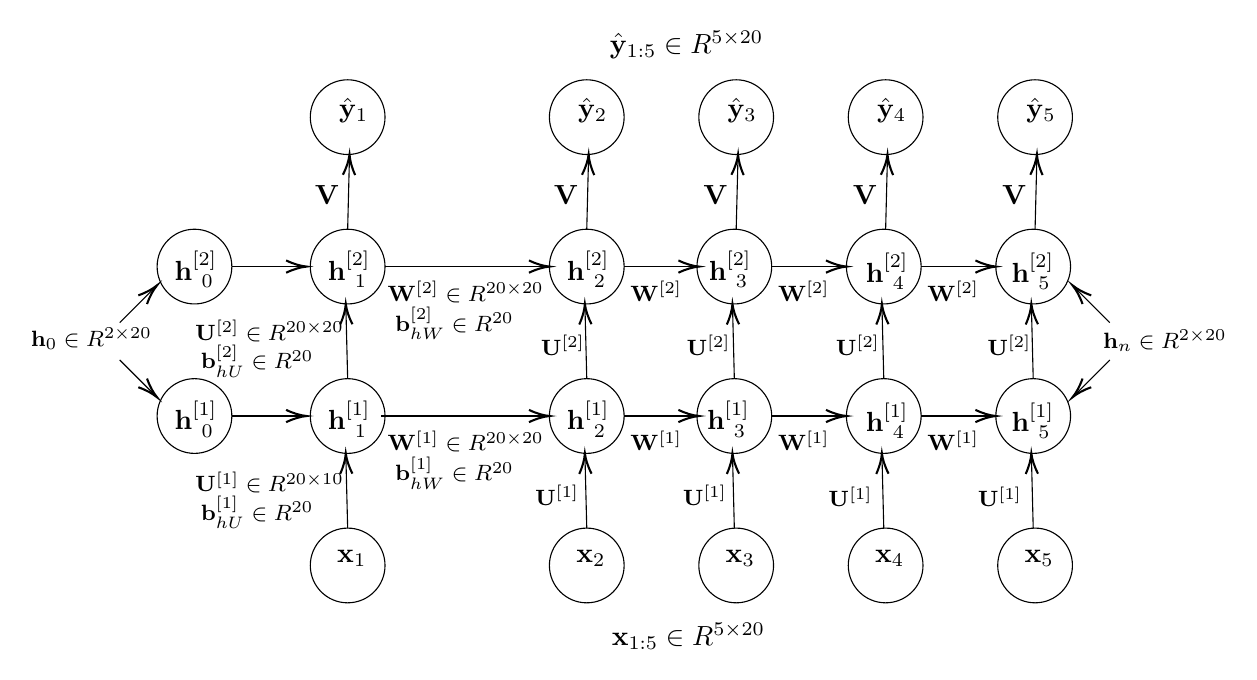
\begin{tikzpicture}[x=0.75pt,y=0.75pt,yscale=-0.9,xscale=0.9] 
        %Shape: Ellipse [id:dp4207915429094031] 
        \draw   (162,300) .. controls (162,288.95) and (170.95,280) .. (182,280) .. controls (193.05,280) and (202,288.95) .. (202,300) .. controls (202,311.05) and (193.05,320) .. (182,320) .. controls (170.95,320) and (162,311.05) .. (162,300) -- cycle ;
        %Straight Lines [id:da05829660867376418] 
        \draw [color={rgb, 255:red, 0; green, 0; blue, 0 }  ,draw opacity=1 ]   (182,280) -- (181.05,242) ;
        \draw [shift={(181,240)}, rotate = 88.57] [color={rgb, 255:red, 0; green, 0; blue, 0 }  ,draw opacity=1 ][line width=0.75]    (10.93,-3.29) .. controls (6.95,-1.4) and (3.31,-0.3) .. (0,0) .. controls (3.31,0.3) and (6.95,1.4) .. (10.93,3.29)   ;
        %Straight Lines [id:da5226654860183346] 
        \draw [color={rgb, 255:red, 0; green, 0; blue, 0 }  ,draw opacity=1 ]   (389,280) -- (388.05,242) ;
        \draw [shift={(388,240)}, rotate = 88.57] [color={rgb, 255:red, 0; green, 0; blue, 0 }  ,draw opacity=1 ][line width=0.75]    (10.93,-3.29) .. controls (6.95,-1.4) and (3.31,-0.3) .. (0,0) .. controls (3.31,0.3) and (6.95,1.4) .. (10.93,3.29)   ;
        %Straight Lines [id:da8260164672182386] 
        \draw [color={rgb, 255:red, 0; green, 0; blue, 0 }  ,draw opacity=1 ]   (469,280) -- (468.05,242) ;
        \draw [shift={(468,240)}, rotate = 88.57] [color={rgb, 255:red, 0; green, 0; blue, 0 }  ,draw opacity=1 ][line width=0.75]    (10.93,-3.29) .. controls (6.95,-1.4) and (3.31,-0.3) .. (0,0) .. controls (3.31,0.3) and (6.95,1.4) .. (10.93,3.29)   ;
        %Straight Lines [id:da9134708342055928] 
        \draw [color={rgb, 255:red, 0; green, 0; blue, 0 }  ,draw opacity=1 ]   (549,280) -- (548.05,242) ;
        \draw [shift={(548,240)}, rotate = 88.57] [color={rgb, 255:red, 0; green, 0; blue, 0 }  ,draw opacity=1 ][line width=0.75]    (10.93,-3.29) .. controls (6.95,-1.4) and (3.31,-0.3) .. (0,0) .. controls (3.31,0.3) and (6.95,1.4) .. (10.93,3.29)   ;
        %Shape: Ellipse [id:dp025885252304979955] 
        \draw   (369,220) .. controls (369,208.95) and (377.95,200) .. (389,200) .. controls (400.05,200) and (409,208.95) .. (409,220) .. controls (409,231.05) and (400.05,240) .. (389,240) .. controls (377.95,240) and (369,231.05) .. (369,220) -- cycle ;
        %Shape: Ellipse [id:dp7180898602484265] 
        \draw   (529,220) .. controls (529,208.95) and (537.95,200) .. (549,200) .. controls (560.05,200) and (569,208.95) .. (569,220) .. controls (569,231.05) and (560.05,240) .. (549,240) .. controls (537.95,240) and (529,231.05) .. (529,220) -- cycle ;
        %Shape: Ellipse [id:dp888584652011154] 
        \draw   (449,220) .. controls (449,208.95) and (457.95,200) .. (469,200) .. controls (480.05,200) and (489,208.95) .. (489,220) .. controls (489,231.05) and (480.05,240) .. (469,240) .. controls (457.95,240) and (449,231.05) .. (449,220) -- cycle ;
        %Shape: Ellipse [id:dp770959326042951] 
        \draw   (162,220) .. controls (162,208.95) and (170.95,200) .. (182,200) .. controls (193.05,200) and (202,208.95) .. (202,220) .. controls (202,231.05) and (193.05,240) .. (182,240) .. controls (170.95,240) and (162,231.05) .. (162,220) -- cycle ;
        %Straight Lines [id:da02863489015429077] 
        \draw [color={rgb, 255:red, 0; green, 0; blue, 0 }  ,draw opacity=1 ]   (409,220) -- (447,220) ;
        \draw [shift={(449,220)}, rotate = 180] [color={rgb, 255:red, 0; green, 0; blue, 0 }  ,draw opacity=1 ][line width=0.75]    (10.93,-3.29) .. controls (6.95,-1.4) and (3.31,-0.3) .. (0,0) .. controls (3.31,0.3) and (6.95,1.4) .. (10.93,3.29)   ;
        %Straight Lines [id:da28454183440455316] 
        \draw [color={rgb, 255:red, 0; green, 0; blue, 0 }  ,draw opacity=1 ]   (489,220) -- (527,220) ;
        \draw [shift={(529,220)}, rotate = 180] [color={rgb, 255:red, 0; green, 0; blue, 0 }  ,draw opacity=1 ][line width=0.75]    (10.93,-3.29) .. controls (6.95,-1.4) and (3.31,-0.3) .. (0,0) .. controls (3.31,0.3) and (6.95,1.4) .. (10.93,3.29)   ;
        %Straight Lines [id:da4244979895569312] 
        \draw [color={rgb, 255:red, 0; green, 0; blue, 0 }  ,draw opacity=1 ]   (182,200) -- (181.05,162) ;
        \draw [shift={(181,160)}, rotate = 88.57] [color={rgb, 255:red, 0; green, 0; blue, 0 }  ,draw opacity=1 ][line width=0.75]    (10.93,-3.29) .. controls (6.95,-1.4) and (3.31,-0.3) .. (0,0) .. controls (3.31,0.3) and (6.95,1.4) .. (10.93,3.29)   ;
        %Straight Lines [id:da41291607651105977] 
        \draw [color={rgb, 255:red, 0; green, 0; blue, 0 }  ,draw opacity=1 ]   (389,200) -- (388.05,162) ;
        \draw [shift={(388,160)}, rotate = 88.57] [color={rgb, 255:red, 0; green, 0; blue, 0 }  ,draw opacity=1 ][line width=0.75]    (10.93,-3.29) .. controls (6.95,-1.4) and (3.31,-0.3) .. (0,0) .. controls (3.31,0.3) and (6.95,1.4) .. (10.93,3.29)   ;
        %Straight Lines [id:da5340101186518054] 
        \draw [color={rgb, 255:red, 0; green, 0; blue, 0 }  ,draw opacity=1 ]   (469,200) -- (468.05,162) ;
        \draw [shift={(468,160)}, rotate = 88.57] [color={rgb, 255:red, 0; green, 0; blue, 0 }  ,draw opacity=1 ][line width=0.75]    (10.93,-3.29) .. controls (6.95,-1.4) and (3.31,-0.3) .. (0,0) .. controls (3.31,0.3) and (6.95,1.4) .. (10.93,3.29)   ;
        %Straight Lines [id:da7929637636987212] 
        \draw [color={rgb, 255:red, 0; green, 0; blue, 0 }  ,draw opacity=1 ]   (549,200) -- (548.05,162) ;
        \draw [shift={(548,160)}, rotate = 88.57] [color={rgb, 255:red, 0; green, 0; blue, 0 }  ,draw opacity=1 ][line width=0.75]    (10.93,-3.29) .. controls (6.95,-1.4) and (3.31,-0.3) .. (0,0) .. controls (3.31,0.3) and (6.95,1.4) .. (10.93,3.29)   ;
        %Shape: Ellipse [id:dp8354295005953776] 
        \draw   (369,140) .. controls (369,128.95) and (377.95,120) .. (389,120) .. controls (400.05,120) and (409,128.95) .. (409,140) .. controls (409,151.05) and (400.05,160) .. (389,160) .. controls (377.95,160) and (369,151.05) .. (369,140) -- cycle ;
        %Shape: Ellipse [id:dp8165367609646754] 
        \draw   (529,140) .. controls (529,128.95) and (537.95,120) .. (549,120) .. controls (560.05,120) and (569,128.95) .. (569,140) .. controls (569,151.05) and (560.05,160) .. (549,160) .. controls (537.95,160) and (529,151.05) .. (529,140) -- cycle ;
        %Shape: Ellipse [id:dp20706274445577244] 
        \draw   (449,140) .. controls (449,128.95) and (457.95,120) .. (469,120) .. controls (480.05,120) and (489,128.95) .. (489,140) .. controls (489,151.05) and (480.05,160) .. (469,160) .. controls (457.95,160) and (449,151.05) .. (449,140) -- cycle ;
        %Shape: Ellipse [id:dp028074370298882823] 
        \draw   (162,140) .. controls (162,128.95) and (170.95,120) .. (182,120) .. controls (193.05,120) and (202,128.95) .. (202,140) .. controls (202,151.05) and (193.05,160) .. (182,160) .. controls (170.95,160) and (162,151.05) .. (162,140) -- cycle ;
        %Straight Lines [id:da40086305523058074] 
        \draw [color={rgb, 255:red, 0; green, 0; blue, 0 }  ,draw opacity=1 ]   (409,140) -- (447,140) ;
        \draw [shift={(449,140)}, rotate = 180] [color={rgb, 255:red, 0; green, 0; blue, 0 }  ,draw opacity=1 ][line width=0.75]    (10.93,-3.29) .. controls (6.95,-1.4) and (3.31,-0.3) .. (0,0) .. controls (3.31,0.3) and (6.95,1.4) .. (10.93,3.29)   ;
        %Straight Lines [id:da3677135880821485] 
        \draw [color={rgb, 255:red, 0; green, 0; blue, 0 }  ,draw opacity=1 ]   (489,140) -- (527,140) ;
        \draw [shift={(529,140)}, rotate = 180] [color={rgb, 255:red, 0; green, 0; blue, 0 }  ,draw opacity=1 ][line width=0.75]    (10.93,-3.29) .. controls (6.95,-1.4) and (3.31,-0.3) .. (0,0) .. controls (3.31,0.3) and (6.95,1.4) .. (10.93,3.29)   ;
        %Shape: Ellipse [id:dp2624210064078889] 
        \draw   (80,140) .. controls (80,128.95) and (88.95,120) .. (100,120) .. controls (111.05,120) and (120,128.95) .. (120,140) .. controls (120,151.05) and (111.05,160) .. (100,160) .. controls (88.95,160) and (80,151.05) .. (80,140) -- cycle ;
        %Straight Lines [id:da4871181057362928] 
        \draw [color={rgb, 255:red, 0; green, 0; blue, 0 }  ,draw opacity=1 ]   (120,140) -- (158,140) ;
        \draw [shift={(160,140)}, rotate = 180] [color={rgb, 255:red, 0; green, 0; blue, 0 }  ,draw opacity=1 ][line width=0.75]    (10.93,-3.29) .. controls (6.95,-1.4) and (3.31,-0.3) .. (0,0) .. controls (3.31,0.3) and (6.95,1.4) .. (10.93,3.29)   ;
        %Shape: Ellipse [id:dp5872757033401736] 
        \draw   (80,220) .. controls (80,208.95) and (88.95,200) .. (100,200) .. controls (111.05,200) and (120,208.95) .. (120,220) .. controls (120,231.05) and (111.05,240) .. (100,240) .. controls (88.95,240) and (80,231.05) .. (80,220) -- cycle ;
        %Straight Lines [id:da2475482028591074] 
        \draw [color={rgb, 255:red, 0; green, 0; blue, 0 }  ,draw opacity=1 ]   (120,220) -- (158,220) ;
        \draw [shift={(160,220)}, rotate = 180] [color={rgb, 255:red, 0; green, 0; blue, 0 }  ,draw opacity=1 ][line width=0.75]    (10.93,-3.29) .. controls (6.95,-1.4) and (3.31,-0.3) .. (0,0) .. controls (3.31,0.3) and (6.95,1.4) .. (10.93,3.29)   ;
        %Straight Lines [id:da9282104785993115] 
        \draw [color={rgb, 255:red, 0; green, 0; blue, 0 }  ,draw opacity=1 ]   (200,220) -- (288,220) ;
        \draw [shift={(290,220)}, rotate = 180] [color={rgb, 255:red, 0; green, 0; blue, 0 }  ,draw opacity=1 ][line width=0.75]    (10.93,-3.29) .. controls (6.95,-1.4) and (3.31,-0.3) .. (0,0) .. controls (3.31,0.3) and (6.95,1.4) .. (10.93,3.29)   ;
        %Straight Lines [id:da17558336312768597] 
        \draw [color={rgb, 255:red, 0; green, 0; blue, 0 }  ,draw opacity=1 ]   (202,140) -- (272,140) -- (288,140) ;
        \draw [shift={(290,140)}, rotate = 180] [color={rgb, 255:red, 0; green, 0; blue, 0 }  ,draw opacity=1 ][line width=0.75]    (10.93,-3.29) .. controls (6.95,-1.4) and (3.31,-0.3) .. (0,0) .. controls (3.31,0.3) and (6.95,1.4) .. (10.93,3.29)   ;
        %Shape: Ellipse [id:dp6255666224284429] 
        \draw   (290,300) .. controls (290,288.95) and (298.95,280) .. (310,280) .. controls (321.05,280) and (330,288.95) .. (330,300) .. controls (330,311.05) and (321.05,320) .. (310,320) .. controls (298.95,320) and (290,311.05) .. (290,300) -- cycle ;
        %Straight Lines [id:da10727200987868368] 
        \draw [color={rgb, 255:red, 0; green, 0; blue, 0 }  ,draw opacity=1 ]   (310,280) -- (309.05,242) ;
        \draw [shift={(309,240)}, rotate = 88.57] [color={rgb, 255:red, 0; green, 0; blue, 0 }  ,draw opacity=1 ][line width=0.75]    (10.93,-3.29) .. controls (6.95,-1.4) and (3.31,-0.3) .. (0,0) .. controls (3.31,0.3) and (6.95,1.4) .. (10.93,3.29)   ;
        %Shape: Ellipse [id:dp8818598215343834] 
        \draw   (290,220) .. controls (290,208.95) and (298.95,200) .. (310,200) .. controls (321.05,200) and (330,208.95) .. (330,220) .. controls (330,231.05) and (321.05,240) .. (310,240) .. controls (298.95,240) and (290,231.05) .. (290,220) -- cycle ;
        %Straight Lines [id:da35172171925239026] 
        \draw [color={rgb, 255:red, 0; green, 0; blue, 0 }  ,draw opacity=1 ]   (310,200) -- (309.05,162) ;
        \draw [shift={(309,160)}, rotate = 88.57] [color={rgb, 255:red, 0; green, 0; blue, 0 }  ,draw opacity=1 ][line width=0.75]    (10.93,-3.29) .. controls (6.95,-1.4) and (3.31,-0.3) .. (0,0) .. controls (3.31,0.3) and (6.95,1.4) .. (10.93,3.29)   ;
        %Shape: Ellipse [id:dp27873635132142716] 
        \draw   (290,140) .. controls (290,128.95) and (298.95,120) .. (310,120) .. controls (321.05,120) and (330,128.95) .. (330,140) .. controls (330,151.05) and (321.05,160) .. (310,160) .. controls (298.95,160) and (290,151.05) .. (290,140) -- cycle ;
        %Straight Lines [id:da38304549426248236] 
        \draw [color={rgb, 255:red, 0; green, 0; blue, 0 }  ,draw opacity=1 ]   (330,220) -- (368,220) ;
        \draw [shift={(370,220)}, rotate = 180] [color={rgb, 255:red, 0; green, 0; blue, 0 }  ,draw opacity=1 ][line width=0.75]    (10.93,-3.29) .. controls (6.95,-1.4) and (3.31,-0.3) .. (0,0) .. controls (3.31,0.3) and (6.95,1.4) .. (10.93,3.29)   ;
        %Straight Lines [id:da57208010142451] 
        \draw [color={rgb, 255:red, 0; green, 0; blue, 0 }  ,draw opacity=1 ]   (330,140) -- (368,140) ;
        \draw [shift={(370,140)}, rotate = 180] [color={rgb, 255:red, 0; green, 0; blue, 0 }  ,draw opacity=1 ][line width=0.75]    (10.93,-3.29) .. controls (6.95,-1.4) and (3.31,-0.3) .. (0,0) .. controls (3.31,0.3) and (6.95,1.4) .. (10.93,3.29)   ;
        %Straight Lines [id:da5663542407709887] 
        \draw [color={rgb, 255:red, 0; green, 0; blue, 0 }  ,draw opacity=1 ]   (390,120) -- (390.95,82) ;
        \draw [shift={(391,80)}, rotate = 91.43] [color={rgb, 255:red, 0; green, 0; blue, 0 }  ,draw opacity=1 ][line width=0.75]    (10.93,-3.29) .. controls (6.95,-1.4) and (3.31,-0.3) .. (0,0) .. controls (3.31,0.3) and (6.95,1.4) .. (10.93,3.29)   ;
        %Straight Lines [id:da32507454347747866] 
        \draw [color={rgb, 255:red, 0; green, 0; blue, 0 }  ,draw opacity=1 ]   (470,120) -- (470.95,82) ;
        \draw [shift={(471,80)}, rotate = 91.43] [color={rgb, 255:red, 0; green, 0; blue, 0 }  ,draw opacity=1 ][line width=0.75]    (10.93,-3.29) .. controls (6.95,-1.4) and (3.31,-0.3) .. (0,0) .. controls (3.31,0.3) and (6.95,1.4) .. (10.93,3.29)   ;
        %Straight Lines [id:da9828329348785247] 
        \draw [color={rgb, 255:red, 0; green, 0; blue, 0 }  ,draw opacity=1 ]   (550,120) -- (550.95,82) ;
        \draw [shift={(551,80)}, rotate = 91.43] [color={rgb, 255:red, 0; green, 0; blue, 0 }  ,draw opacity=1 ][line width=0.75]    (10.93,-3.29) .. controls (6.95,-1.4) and (3.31,-0.3) .. (0,0) .. controls (3.31,0.3) and (6.95,1.4) .. (10.93,3.29)   ;
        %Straight Lines [id:da21940187807374456] 
        \draw [color={rgb, 255:red, 0; green, 0; blue, 0 }  ,draw opacity=1 ]   (182,120) -- (182.95,82) ;
        \draw [shift={(183,80)}, rotate = 91.43] [color={rgb, 255:red, 0; green, 0; blue, 0 }  ,draw opacity=1 ][line width=0.75]    (10.93,-3.29) .. controls (6.95,-1.4) and (3.31,-0.3) .. (0,0) .. controls (3.31,0.3) and (6.95,1.4) .. (10.93,3.29)   ;
        %Straight Lines [id:da9515990853220169] 
        \draw [color={rgb, 255:red, 0; green, 0; blue, 0 }  ,draw opacity=1 ]   (310,120) -- (310.95,82) ;
        \draw [shift={(311,80)}, rotate = 91.43] [color={rgb, 255:red, 0; green, 0; blue, 0 }  ,draw opacity=1 ][line width=0.75]    (10.93,-3.29) .. controls (6.95,-1.4) and (3.31,-0.3) .. (0,0) .. controls (3.31,0.3) and (6.95,1.4) .. (10.93,3.29)   ;
        %Shape: Ellipse [id:dp7031207995591184] 
        \draw   (162,60) .. controls (162,48.95) and (170.95,40) .. (182,40) .. controls (193.05,40) and (202,48.95) .. (202,60) .. controls (202,71.05) and (193.05,80) .. (182,80) .. controls (170.95,80) and (162,71.05) .. (162,60) -- cycle ;
        %Shape: Ellipse [id:dp4918664633020191] 
        \draw   (290,60) .. controls (290,48.95) and (298.95,40) .. (310,40) .. controls (321.05,40) and (330,48.95) .. (330,60) .. controls (330,71.05) and (321.05,80) .. (310,80) .. controls (298.95,80) and (290,71.05) .. (290,60) -- cycle ;
        %Shape: Ellipse [id:dp678788283809618] 
        \draw   (370,60) .. controls (370,48.95) and (378.95,40) .. (390,40) .. controls (401.05,40) and (410,48.95) .. (410,60) .. controls (410,71.05) and (401.05,80) .. (390,80) .. controls (378.95,80) and (370,71.05) .. (370,60) -- cycle ;
        %Shape: Ellipse [id:dp40410246110864323] 
        \draw   (450,60) .. controls (450,48.95) and (458.95,40) .. (470,40) .. controls (481.05,40) and (490,48.95) .. (490,60) .. controls (490,71.05) and (481.05,80) .. (470,80) .. controls (458.95,80) and (450,71.05) .. (450,60) -- cycle ;
        %Shape: Ellipse [id:dp357818602045721] 
        \draw   (530,60) .. controls (530,48.95) and (538.95,40) .. (550,40) .. controls (561.05,40) and (570,48.95) .. (570,60) .. controls (570,71.05) and (561.05,80) .. (550,80) .. controls (538.95,80) and (530,71.05) .. (530,60) -- cycle ;
        %Shape: Ellipse [id:dp861370706015621] 
        \draw   (370,300) .. controls (370,288.95) and (378.95,280) .. (390,280) .. controls (401.05,280) and (410,288.95) .. (410,300) .. controls (410,311.05) and (401.05,320) .. (390,320) .. controls (378.95,320) and (370,311.05) .. (370,300) -- cycle ;
        %Shape: Ellipse [id:dp10149404856059419] 
        \draw   (450,300) .. controls (450,288.95) and (458.95,280) .. (470,280) .. controls (481.05,280) and (490,288.95) .. (490,300) .. controls (490,311.05) and (481.05,320) .. (470,320) .. controls (458.95,320) and (450,311.05) .. (450,300) -- cycle ;
        %Shape: Ellipse [id:dp5054375673565727] 
        \draw   (530,300) .. controls (530,288.95) and (538.95,280) .. (550,280) .. controls (561.05,280) and (570,288.95) .. (570,300) .. controls (570,311.05) and (561.05,320) .. (550,320) .. controls (538.95,320) and (530,311.05) .. (530,300) -- cycle ;
        %Straight Lines [id:da48642808985309793] 
        \draw    (60,170) -- (78.59,151.41) ;
        \draw [shift={(80,150)}, rotate = 135] [color={rgb, 255:red, 0; green, 0; blue, 0 }  ][line width=0.75]    (10.93,-3.29) .. controls (6.95,-1.4) and (3.31,-0.3) .. (0,0) .. controls (3.31,0.3) and (6.95,1.4) .. (10.93,3.29)   ;
        %Straight Lines [id:da622558990053925] 
        \draw    (60,190) -- (78.59,208.59) ;
        \draw [shift={(80,210)}, rotate = 225] [color={rgb, 255:red, 0; green, 0; blue, 0 }  ][line width=0.75]    (10.93,-3.29) .. controls (6.95,-1.4) and (3.31,-0.3) .. (0,0) .. controls (3.31,0.3) and (6.95,1.4) .. (10.93,3.29)   ;
        %Straight Lines [id:da4475932343558764] 
        \draw    (590,170) -- (571.41,151.41) ;
        \draw [shift={(570,150)}, rotate = 45] [color={rgb, 255:red, 0; green, 0; blue, 0 }  ][line width=0.75]    (10.93,-3.29) .. controls (6.95,-1.4) and (3.31,-0.3) .. (0,0) .. controls (3.31,0.3) and (6.95,1.4) .. (10.93,3.29)   ;
        %Straight Lines [id:da7531844960895331] 
        \draw    (590,190) -- (571.41,208.59) ;
        \draw [shift={(570,210)}, rotate = 315] [color={rgb, 255:red, 0; green, 0; blue, 0 }  ][line width=0.75]    (10.93,-3.29) .. controls (6.95,-1.4) and (3.31,-0.3) .. (0,0) .. controls (3.31,0.3) and (6.95,1.4) .. (10.93,3.29)   ;

        % Text Node
        \draw (175,290.4) node [anchor=north west][inner sep=0.75pt]  [font=\normalsize]  {$\mathbf{x}_{1}$};
        % Text Node
        \draw (360,255.4) node [anchor=north west][inner sep=0.75pt]  [font=\footnotesize,color={rgb, 255:red, 0; green, 0; blue, 0 }  ,opacity=1 ]  {$\mathbf{U}^{[ 1]}$};
        % Text Node
        \draw (438,256.4) node [anchor=north west][inner sep=0.75pt]  [font=\footnotesize,color={rgb, 255:red, 0; green, 0; blue, 0 }  ,opacity=1 ]  {$\mathbf{U}^{[ 1]}$};
        % Text Node
        \draw (518,256.4) node [anchor=north west][inner sep=0.75pt]  [font=\footnotesize,color={rgb, 255:red, 0; green, 0; blue, 0 }  ,opacity=1 ]  {$\mathbf{U}^{[ 1]}$};
        % Text Node
        \draw (170,210.4) node [anchor=north west][inner sep=0.75pt]  [font=\normalsize]  {$\mathbf{h}_{\ 1}^{[ 1]}$};
        % Text Node
        \draw (373,210.4) node [anchor=north west][inner sep=0.75pt]  [font=\normalsize]  {$\mathbf{h}_{\ 3}^{[ 1]}$};
        % Text Node
        \draw (458,211.4) node [anchor=north west][inner sep=0.75pt]  [font=\normalsize]  {$\mathbf{h}_{\ 4}^{[ 1]}$};
        % Text Node
        \draw (536,211.4) node [anchor=north west][inner sep=0.75pt]  [font=\normalsize]  {$\mathbf{h}_{\ 5}^{[ 1]}$};
        % Text Node
        \draw (411,226.4) node [anchor=north west][inner sep=0.75pt]  [font=\footnotesize,color={rgb, 255:red, 0; green, 0; blue, 0 }  ,opacity=1 ]  {$\mathbf{W}^{[ 1]}$};
        % Text Node
        \draw (491,226.4) node [anchor=north west][inner sep=0.75pt]  [font=\footnotesize,color={rgb, 255:red, 0; green, 0; blue, 0 }  ,opacity=1 ]  {$\mathbf{W}^{[ 1]}$};
        % Text Node
        \draw (99,167.4) node [anchor=north west][inner sep=0.75pt]  [font=\footnotesize,color={rgb, 255:red, 0; green, 0; blue, 0 }  ,opacity=1 ]  {$\mathbf{U}^{[ 2]} \in \mathbb{R}^{20\times 20}$};
        % Text Node
        \draw (362,175.4) node [anchor=north west][inner sep=0.75pt]  [font=\footnotesize,color={rgb, 255:red, 0; green, 0; blue, 0 }  ,opacity=1 ]  {$\mathbf{U}^{[ 2]}$};
        % Text Node
        \draw (442,175.4) node [anchor=north west][inner sep=0.75pt]  [font=\footnotesize,color={rgb, 255:red, 0; green, 0; blue, 0 }  ,opacity=1 ]  {$\mathbf{U}^{[ 2]}$};
        % Text Node
        \draw (523,175.4) node [anchor=north west][inner sep=0.75pt]  [font=\footnotesize,color={rgb, 255:red, 0; green, 0; blue, 0 }  ,opacity=1 ]  {$\mathbf{U}^{[ 2]}$};
        % Text Node
        \draw (170,130.4) node [anchor=north west][inner sep=0.75pt]  [font=\normalsize]  {$\mathbf{h}_{\ 1}^{[ 2]}$};
        % Text Node
        \draw (374,130.4) node [anchor=north west][inner sep=0.75pt]  [font=\normalsize]  {$\mathbf{h}_{\ 3}^{[ 2]}$};
        % Text Node
        \draw (458,131.4) node [anchor=north west][inner sep=0.75pt]  [font=\normalsize]  {$\mathbf{h}_{\ 4}^{[ 2]}$};
        % Text Node
        \draw (536,131.4) node [anchor=north west][inner sep=0.75pt]  [font=\normalsize]  {$\mathbf{h}_{\ 5}^{[ 2]}$};
        % Text Node
        \draw (411,146.4) node [anchor=north west][inner sep=0.75pt]  [font=\footnotesize,color={rgb, 255:red, 0; green, 0; blue, 0 }  ,opacity=1 ]  {$\mathbf{W}^{[ 2]}$};
        % Text Node
        \draw (491,146.4) node [anchor=north west][inner sep=0.75pt]  [font=\footnotesize,color={rgb, 255:red, 0; green, 0; blue, 0 }  ,opacity=1 ]  {$\mathbf{W}^{[ 2]}$};
        % Text Node
        \draw (88,130.4) node [anchor=north west][inner sep=0.75pt]  [font=\normalsize]  {$\mathbf{h}_{\ 0}^{[ 2]}$};
        % Text Node
        \draw (88,210.4) node [anchor=north west][inner sep=0.75pt]  [font=\normalsize]  {$\mathbf{h}_{\ 0}^{[ 1]}$};
        % Text Node
        \draw (202,146.4) node [anchor=north west][inner sep=0.75pt]  [font=\footnotesize,color={rgb, 255:red, 0; green, 0; blue, 0 }  ,opacity=1 ]  {$\mathbf{W}^{[ 2]} \in \mathbb{R}^{20\times 20}$};
        % Text Node
        \draw (303,290.4) node [anchor=north west][inner sep=0.75pt]  [font=\normalsize]  {$\mathbf{x}_{2}$};
        % Text Node
        \draw (281,255.4) node [anchor=north west][inner sep=0.75pt]  [font=\footnotesize,color={rgb, 255:red, 0; green, 0; blue, 0 }  ,opacity=1 ]  {$\mathbf{U}^{[ 1]}$};
        % Text Node
        \draw (298,210.4) node [anchor=north west][inner sep=0.75pt]  [font=\normalsize]  {$\mathbf{h}_{\ 2}^{[ 1]}$};
        % Text Node
        \draw (284,175.4) node [anchor=north west][inner sep=0.75pt]  [font=\footnotesize,color={rgb, 255:red, 0; green, 0; blue, 0 }  ,opacity=1 ]  {$\mathbf{U}^{[ 2]}$};
        % Text Node
        \draw (298,130.4) node [anchor=north west][inner sep=0.75pt]  [font=\normalsize]  {$\mathbf{h}_{\ 2}^{[ 2]}$};
        % Text Node
        \draw (332,226.4) node [anchor=north west][inner sep=0.75pt]  [font=\footnotesize,color={rgb, 255:red, 0; green, 0; blue, 0 }  ,opacity=1 ]  {$\mathbf{W}^{[ 1]}$};
        % Text Node
        \draw (332,146.4) node [anchor=north west][inner sep=0.75pt]  [font=\footnotesize,color={rgb, 255:red, 0; green, 0; blue, 0 }  ,opacity=1 ]  {$\mathbf{W}^{[ 2]}$};
        % Text Node
        \draw (371,95.4) node [anchor=north west][inner sep=0.75pt]  [font=\normalsize,color={rgb, 255:red, 0; green, 0; blue, 0 }  ,opacity=1 ]  {$\mathbf{V}$};
        % Text Node
        \draw (451,95.4) node [anchor=north west][inner sep=0.75pt]  [font=\normalsize,color={rgb, 255:red, 0; green, 0; blue, 0 }  ,opacity=1 ]  {$\mathbf{V}$};
        % Text Node
        \draw (531,95.4) node [anchor=north west][inner sep=0.75pt]  [font=\normalsize,color={rgb, 255:red, 0; green, 0; blue, 0 }  ,opacity=1 ]  {$\mathbf{V}$};
        % Text Node
        \draw (163,95.4) node [anchor=north west][inner sep=0.75pt]  [font=\normalsize,color={rgb, 255:red, 0; green, 0; blue, 0 }  ,opacity=1 ]  {$\mathbf{V}$};
        % Text Node
        \draw (291,95.4) node [anchor=north west][inner sep=0.75pt]  [font=\normalsize,color={rgb, 255:red, 0; green, 0; blue, 0 }  ,opacity=1 ]  {$\mathbf{V}$};
        % Text Node
        \draw (176,48.4) node [anchor=north west][inner sep=0.75pt]  [font=\normalsize]  {$\hat{\mathbf{y}}_{1}$};
        % Text Node
        \draw (304,48.4) node [anchor=north west][inner sep=0.75pt]  [font=\normalsize]  {$\hat{\mathbf{y}}_{2}$};
        % Text Node
        \draw (384,48.4) node [anchor=north west][inner sep=0.75pt]  [font=\normalsize]  {$\hat{\mathbf{y}}_{3}$};
        % Text Node
        \draw (464,48.4) node [anchor=north west][inner sep=0.75pt]  [font=\normalsize]  {$\hat{\mathbf{y}}_{4}$};
        % Text Node
        \draw (544,48.4) node [anchor=north west][inner sep=0.75pt]  [font=\normalsize]  {$\hat{\mathbf{y}}_{5}$};
        % Text Node
        \draw (383,290.4) node [anchor=north west][inner sep=0.75pt]  [font=\normalsize]  {$\mathbf{x}_{3}$};
        % Text Node
        \draw (463,290.4) node [anchor=north west][inner sep=0.75pt]  [font=\normalsize]  {$\mathbf{x}_{4}$};
        % Text Node
        \draw (543,290.4) node [anchor=north west][inner sep=0.75pt]  [font=\normalsize]  {$\mathbf{x}_{5}$};
        % Text Node
        \draw (202,226.4) node [anchor=north west][inner sep=0.75pt]  [font=\footnotesize,color={rgb, 255:red, 0; green, 0; blue, 0 }  ,opacity=1 ]  {$\mathbf{W}^{[ 1]} \in \mathbb{R}^{20\times 20}$};
        % Text Node
        \draw (99,248.4) node [anchor=north west][inner sep=0.75pt]  [font=\footnotesize,color={rgb, 255:red, 0; green, 0; blue, 0 }  ,opacity=1 ]  {$\mathbf{U}^{[ 1]} \in \mathbb{R}^{20\times 10}$};
        % Text Node
        \draw (102,261.4) node [anchor=north west][inner sep=0.75pt]  [font=\footnotesize,color={rgb, 255:red, 0; green, 0; blue, 0 }  ,opacity=1 ]  {$\mathbf{b}_{hU}^{[ 1]} \in \mathbb{R}^{20}$};
        % Text Node
        \draw (102,180.4) node [anchor=north west][inner sep=0.75pt]  [font=\footnotesize,color={rgb, 255:red, 0; green, 0; blue, 0 }  ,opacity=1 ]  {$\mathbf{b}_{hU}^{[ 2]} \in \mathbb{R}^{20}$};
        % Text Node
        \draw (206,160.4) node [anchor=north west][inner sep=0.75pt]  [font=\footnotesize,color={rgb, 255:red, 0; green, 0; blue, 0 }  ,opacity=1 ]  {$\mathbf{b}_{hW}^{[ 2]} \in \mathbb{R}^{20}$};
        % Text Node
        \draw (206,240.4) node [anchor=north west][inner sep=0.75pt]  [font=\footnotesize,color={rgb, 255:red, 0; green, 0; blue, 0 }  ,opacity=1 ]  {$\mathbf{b}_{hW}^{[ 1]} \in \mathbb{R}^{20}$};
        % Text Node
        \draw (11,171.4) node [anchor=north west][inner sep=0.75pt]  [font=\footnotesize]  {$\mathbf{h}_{0} \in \mathbb{R}^{2\times 20}$};
        % Text Node
        \draw (585,172.4) node [anchor=north west][inner sep=0.75pt]  [font=\footnotesize]  {$\mathbf{h}_{n} \in \mathbb{R}^{2\times 20}$};
        % Text Node
        \draw (322,329.4) node [anchor=north west][inner sep=0.75pt]  [font=\normalsize]  {$\mathbf{x}_{1:5} \in \mathbb{R}^{5\times 20}$};
        % Text Node
        \draw (321,12.4) node [anchor=north west][inner sep=0.75pt]  [font=\normalsize]  {$\hat{\mathbf{y}}_{1:5} \in \mathbb{R}^{5\times 20}$};
      \end{tikzpicture}
      \caption{}
      \label{fig:rnn_pytorch_rnn}
    \end{figure}

    As we expect, there are 8 vectors/matrices we must optimize: $\mathbf{W}^{[1]}, \mathbf{W}^{[2]}, \mathbf{U}^{[1]}, \mathbf{U}^{[2]}, \mathbf{b}^{[1]}_{hU}, \mathbf{b}^{[1]}_{hW}, \mathbf{b}^{[2]}_{hW}, \mathbf{b}^{[2]}_{hU}$. 

\subsection{Long Short Term Memory (LSTMs)}

  In theory, RNNs are very beautiful and can be applied in all cases, but in practice they do not perform very well, mainly due to the vanishing/exploding gradient problem. 
  \begin{enumerate}
    \item An exploding gradient is easy to fix, since we can just use the max-norm regularization, i.e. \textbf{gradient clipping}, to just set a max vamlue for the gradients if they grow too large. 
    \item The \textbf{truncated backpropagation through time} (TBPTT) simply limits the number of times steps the signal can backpropagate after each forward pass, e.g. even if the sequence has 100 time steps, we may only backpropagate through 20 or so. 
    \item The \textbf{LSTM} model uses a memory cell for modeling long-range dependencies and avoids the vanishing gradient problems. 
  \end{enumerate}

  Historically LSTMs were used in achieving state-of-the-art results in 2013 through 2015, in tasks such as handwriting recognition, speech recognition, machine translation, parsing, and image captioning, as well as language models. They became to dominant approach for most NLP tasks, but in 2021, they have been overshadowed by transformer models, which we will talk about next. 

  LSTMs have a much more complicated unit to work with, so let's go through it slowly. Note that so far, a one-layer RNN consisted of recursive mappings of the form 
  \begin{equation}
    (\mathbf{x}_t, \mathbf{h}_{t-1}) \mapsto ( \mathbf{h}_t, \hat{\mathbf{y}}_t)
  \end{equation}
  We can interpret the vector $\mathbf{h}_{t-1}$ as the \textbf{short term memory}, or \textbf{hidden state}, that contains information used to predict the next output value. However, this can be corrupted (e.g. forgetting information from many steps ago), so we add an additional \textbf{long term memory}, or \textbf{cell state}, vector $\mathbf{c}_t$ that should be preserved. Therefore, we have two arrows coming out of each hidden layer, as shown below in the one-layer LSTM. 

  \begin{figure}[H]
    \centering 
    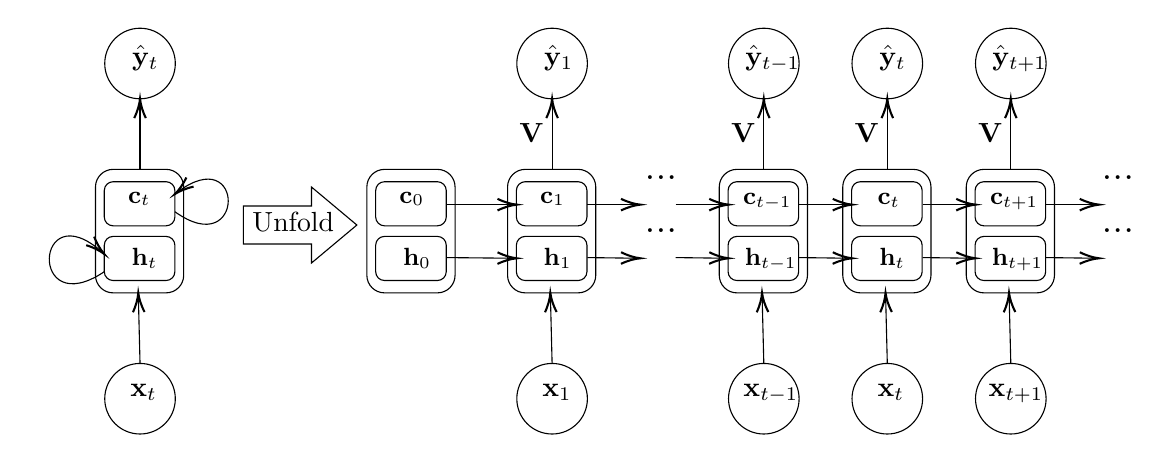
\begin{tikzpicture}[x=0.75pt,y=0.75pt,yscale=-0.85,xscale=0.85]
      %Rounded Rect [id:dp9162379150448552] 
      \draw   (36.18,110) .. controls (36.18,104.48) and (40.66,100) .. (46.18,100) -- (76.18,100) .. controls (81.71,100) and (86.18,104.48) .. (86.18,110) -- (86.18,160) .. controls (86.18,165.52) and (81.71,170) .. (76.18,170) -- (46.18,170) .. controls (40.66,170) and (36.18,165.52) .. (36.18,160) -- cycle ;
      %Rounded Rect [id:dp44390871530521614] 
      \draw   (41.18,112) .. controls (41.18,109.24) and (43.42,107) .. (46.18,107) -- (76.18,107) .. controls (78.95,107) and (81.18,109.24) .. (81.18,112) -- (81.18,127) .. controls (81.18,129.76) and (78.95,132) .. (76.18,132) -- (46.18,132) .. controls (43.42,132) and (41.18,129.76) .. (41.18,127) -- cycle ;
      %Rounded Rect [id:dp023212849697244353] 
      \draw   (41.18,143) .. controls (41.18,140.24) and (43.42,138) .. (46.18,138) -- (76.18,138) .. controls (78.95,138) and (81.18,140.24) .. (81.18,143) -- (81.18,158) .. controls (81.18,160.76) and (78.95,163) .. (76.18,163) -- (46.18,163) .. controls (43.42,163) and (41.18,160.76) .. (41.18,158) -- cycle ;
      %Curve Lines [id:da46664761054448833] 
      \draw [color={rgb, 255:red, 0; green, 0; blue, 0 }  ,draw opacity=1 ]   (81.18,124) .. controls (121.11,152.71) and (121.51,83.41) .. (82.38,113.07) ;
      \draw [shift={(81.18,114)}, rotate = 321.57] [color={rgb, 255:red, 0; green, 0; blue, 0 }  ,draw opacity=1 ][line width=0.75]    (10.93,-3.29) .. controls (6.95,-1.4) and (3.31,-0.3) .. (0,0) .. controls (3.31,0.3) and (6.95,1.4) .. (10.93,3.29)   ;
      %Curve Lines [id:da10224295018656915] 
      \draw [color={rgb, 255:red, 0; green, 0; blue, 0 }  ,draw opacity=1 ]   (41.18,158) .. controls (-1.94,186.93) and (1.55,112.73) .. (40.01,146.93) ;
      \draw [shift={(41.18,148)}, rotate = 222.92] [color={rgb, 255:red, 0; green, 0; blue, 0 }  ,draw opacity=1 ][line width=0.75]    (10.93,-3.29) .. controls (6.95,-1.4) and (3.31,-0.3) .. (0,0) .. controls (3.31,0.3) and (6.95,1.4) .. (10.93,3.29)   ;
      %Shape: Ellipse [id:dp6111375564351242] 
      \draw   (41.43,40) .. controls (41.43,28.95) and (50.39,20) .. (61.43,20) .. controls (72.48,20) and (81.43,28.95) .. (81.43,40) .. controls (81.43,51.05) and (72.48,60) .. (61.43,60) .. controls (50.39,60) and (41.43,51.05) .. (41.43,40) -- cycle ;
      %Straight Lines [id:da9695643363673832] 
      \draw [color={rgb, 255:red, 0; green, 0; blue, 0 }  ,draw opacity=1 ]   (61.43,100) -- (61.43,66) -- (61.43,62) ;
      \draw [shift={(61.43,60)}, rotate = 90] [color={rgb, 255:red, 0; green, 0; blue, 0 }  ,draw opacity=1 ][line width=0.75]    (10.93,-3.29) .. controls (6.95,-1.4) and (3.31,-0.3) .. (0,0) .. controls (3.31,0.3) and (6.95,1.4) .. (10.93,3.29)   ;
      %Shape: Ellipse [id:dp32272156031695665] 
      \draw   (41.43,230) .. controls (41.43,218.95) and (50.39,210) .. (61.43,210) .. controls (72.48,210) and (81.43,218.95) .. (81.43,230) .. controls (81.43,241.05) and (72.48,250) .. (61.43,250) .. controls (50.39,250) and (41.43,241.05) .. (41.43,230) -- cycle ;
      %Straight Lines [id:da915552261165167] 
      \draw [color={rgb, 255:red, 0; green, 0; blue, 0 }  ,draw opacity=1 ]   (61.43,210) -- (60.48,172) ;
      \draw [shift={(60.43,170)}, rotate = 88.57] [color={rgb, 255:red, 0; green, 0; blue, 0 }  ,draw opacity=1 ][line width=0.75]    (10.93,-3.29) .. controls (6.95,-1.4) and (3.31,-0.3) .. (0,0) .. controls (3.31,0.3) and (6.95,1.4) .. (10.93,3.29)   ;
      %Rounded Rect [id:dp8652549705300117] 
      \draw   (269.75,110) .. controls (269.75,104.48) and (274.23,100) .. (279.75,100) -- (309.75,100) .. controls (315.27,100) and (319.75,104.48) .. (319.75,110) -- (319.75,160) .. controls (319.75,165.52) and (315.27,170) .. (309.75,170) -- (279.75,170) .. controls (274.23,170) and (269.75,165.52) .. (269.75,160) -- cycle ;
      %Rounded Rect [id:dp822911802732121] 
      \draw   (274.75,112) .. controls (274.75,109.24) and (276.99,107) .. (279.75,107) -- (309.75,107) .. controls (312.51,107) and (314.75,109.24) .. (314.75,112) -- (314.75,127) .. controls (314.75,129.76) and (312.51,132) .. (309.75,132) -- (279.75,132) .. controls (276.99,132) and (274.75,129.76) .. (274.75,127) -- cycle ;
      %Rounded Rect [id:dp4389013645428701] 
      \draw   (274.75,143) .. controls (274.75,140.24) and (276.99,138) .. (279.75,138) -- (309.75,138) .. controls (312.51,138) and (314.75,140.24) .. (314.75,143) -- (314.75,158) .. controls (314.75,160.76) and (312.51,163) .. (309.75,163) -- (279.75,163) .. controls (276.99,163) and (274.75,160.76) .. (274.75,158) -- cycle ;
      %Shape: Ellipse [id:dp5525645091420477] 
      \draw   (275,40) .. controls (275,28.95) and (283.95,20) .. (295,20) .. controls (306.05,20) and (315,28.95) .. (315,40) .. controls (315,51.05) and (306.05,60) .. (295,60) .. controls (283.95,60) and (275,51.05) .. (275,40) -- cycle ;
      %Straight Lines [id:da2804916545696292] 
      \draw [color={rgb, 255:red, 0; green, 0; blue, 0 }  ,draw opacity=1 ]   (295,100) -- (295,66) -- (295,62) ;
      \draw [shift={(295,60)}, rotate = 90] [color={rgb, 255:red, 0; green, 0; blue, 0 }  ,draw opacity=1 ][line width=0.75]    (10.93,-3.29) .. controls (6.95,-1.4) and (3.31,-0.3) .. (0,0) .. controls (3.31,0.3) and (6.95,1.4) .. (10.93,3.29)   ;
      %Shape: Ellipse [id:dp965284018613916] 
      \draw   (275,230) .. controls (275,218.95) and (283.95,210) .. (295,210) .. controls (306.05,210) and (315,218.95) .. (315,230) .. controls (315,241.05) and (306.05,250) .. (295,250) .. controls (283.95,250) and (275,241.05) .. (275,230) -- cycle ;
      %Straight Lines [id:da9987984073296703] 
      \draw [color={rgb, 255:red, 0; green, 0; blue, 0 }  ,draw opacity=1 ]   (295,210) -- (294.05,172) ;
      \draw [shift={(294,170)}, rotate = 88.57] [color={rgb, 255:red, 0; green, 0; blue, 0 }  ,draw opacity=1 ][line width=0.75]    (10.93,-3.29) .. controls (6.95,-1.4) and (3.31,-0.3) .. (0,0) .. controls (3.31,0.3) and (6.95,1.4) .. (10.93,3.29)   ;
      %Rounded Rect [id:dp9014606046524996] 
      \draw   (190,110) .. controls (190,104.48) and (194.48,100) .. (200,100) -- (230,100) .. controls (235.52,100) and (240,104.48) .. (240,110) -- (240,160) .. controls (240,165.52) and (235.52,170) .. (230,170) -- (200,170) .. controls (194.48,170) and (190,165.52) .. (190,160) -- cycle ;
      %Rounded Rect [id:dp3774395803757169] 
      \draw   (195,112) .. controls (195,109.24) and (197.24,107) .. (200,107) -- (230,107) .. controls (232.76,107) and (235,109.24) .. (235,112) -- (235,127) .. controls (235,129.76) and (232.76,132) .. (230,132) -- (200,132) .. controls (197.24,132) and (195,129.76) .. (195,127) -- cycle ;
      %Rounded Rect [id:dp45599758014939185] 
      \draw   (195,143) .. controls (195,140.24) and (197.24,138) .. (200,138) -- (230,138) .. controls (232.76,138) and (235,140.24) .. (235,143) -- (235,158) .. controls (235,160.76) and (232.76,163) .. (230,163) -- (200,163) .. controls (197.24,163) and (195,160.76) .. (195,158) -- cycle ;
      %Straight Lines [id:da7966139010055635] 
      \draw [color={rgb, 255:red, 0; green, 0; blue, 0 }  ,draw opacity=1 ]   (235,120) -- (273,120) ;
      \draw [shift={(275,120)}, rotate = 180] [color={rgb, 255:red, 0; green, 0; blue, 0 }  ,draw opacity=1 ][line width=0.75]    (10.93,-3.29) .. controls (6.95,-1.4) and (3.31,-0.3) .. (0,0) .. controls (3.31,0.3) and (6.95,1.4) .. (10.93,3.29)   ;
      %Straight Lines [id:da45720187180824867] 
      \draw [color={rgb, 255:red, 0; green, 0; blue, 0 }  ,draw opacity=1 ]   (235,150) -- (273,150.38) ;
      \draw [shift={(275,150.4)}, rotate = 180.57] [color={rgb, 255:red, 0; green, 0; blue, 0 }  ,draw opacity=1 ][line width=0.75]    (10.93,-3.29) .. controls (6.95,-1.4) and (3.31,-0.3) .. (0,0) .. controls (3.31,0.3) and (6.95,1.4) .. (10.93,3.29)   ;
      %Rounded Rect [id:dp460830929796783] 
      \draw   (389.75,110) .. controls (389.75,104.48) and (394.23,100) .. (399.75,100) -- (429.75,100) .. controls (435.27,100) and (439.75,104.48) .. (439.75,110) -- (439.75,160) .. controls (439.75,165.52) and (435.27,170) .. (429.75,170) -- (399.75,170) .. controls (394.23,170) and (389.75,165.52) .. (389.75,160) -- cycle ;
      %Rounded Rect [id:dp4723457857148323] 
      \draw   (394.75,112) .. controls (394.75,109.24) and (396.99,107) .. (399.75,107) -- (429.75,107) .. controls (432.51,107) and (434.75,109.24) .. (434.75,112) -- (434.75,127) .. controls (434.75,129.76) and (432.51,132) .. (429.75,132) -- (399.75,132) .. controls (396.99,132) and (394.75,129.76) .. (394.75,127) -- cycle ;
      %Rounded Rect [id:dp33200733080738165] 
      \draw   (394.75,143) .. controls (394.75,140.24) and (396.99,138) .. (399.75,138) -- (429.75,138) .. controls (432.51,138) and (434.75,140.24) .. (434.75,143) -- (434.75,158) .. controls (434.75,160.76) and (432.51,163) .. (429.75,163) -- (399.75,163) .. controls (396.99,163) and (394.75,160.76) .. (394.75,158) -- cycle ;
      %Straight Lines [id:da5193373762807063] 
      \draw [color={rgb, 255:red, 0; green, 0; blue, 0 }  ,draw opacity=1 ]   (415,100) -- (415,66) -- (415,62) ;
      \draw [shift={(415,60)}, rotate = 90] [color={rgb, 255:red, 0; green, 0; blue, 0 }  ,draw opacity=1 ][line width=0.75]    (10.93,-3.29) .. controls (6.95,-1.4) and (3.31,-0.3) .. (0,0) .. controls (3.31,0.3) and (6.95,1.4) .. (10.93,3.29)   ;
      %Straight Lines [id:da9854180431917805] 
      \draw [color={rgb, 255:red, 0; green, 0; blue, 0 }  ,draw opacity=1 ]   (415,210) -- (414.05,172) ;
      \draw [shift={(414,170)}, rotate = 88.57] [color={rgb, 255:red, 0; green, 0; blue, 0 }  ,draw opacity=1 ][line width=0.75]    (10.93,-3.29) .. controls (6.95,-1.4) and (3.31,-0.3) .. (0,0) .. controls (3.31,0.3) and (6.95,1.4) .. (10.93,3.29)   ;
      %Straight Lines [id:da9743940552021377] 
      \draw [color={rgb, 255:red, 0; green, 0; blue, 0 }  ,draw opacity=1 ]   (365,120) -- (393,120) ;
      \draw [shift={(395,120)}, rotate = 180] [color={rgb, 255:red, 0; green, 0; blue, 0 }  ,draw opacity=1 ][line width=0.75]    (10.93,-3.29) .. controls (6.95,-1.4) and (3.31,-0.3) .. (0,0) .. controls (3.31,0.3) and (6.95,1.4) .. (10.93,3.29)   ;
      %Straight Lines [id:da49268195029439243] 
      \draw [color={rgb, 255:red, 0; green, 0; blue, 0 }  ,draw opacity=1 ]   (365,150) -- (393,150.37) ;
      \draw [shift={(395,150.4)}, rotate = 180.76] [color={rgb, 255:red, 0; green, 0; blue, 0 }  ,draw opacity=1 ][line width=0.75]    (10.93,-3.29) .. controls (6.95,-1.4) and (3.31,-0.3) .. (0,0) .. controls (3.31,0.3) and (6.95,1.4) .. (10.93,3.29)   ;
      %Straight Lines [id:da10388697103876177] 
      \draw [color={rgb, 255:red, 0; green, 0; blue, 0 }  ,draw opacity=1 ]   (315,120) -- (343,120) ;
      \draw [shift={(345,120)}, rotate = 180] [color={rgb, 255:red, 0; green, 0; blue, 0 }  ,draw opacity=1 ][line width=0.75]    (10.93,-3.29) .. controls (6.95,-1.4) and (3.31,-0.3) .. (0,0) .. controls (3.31,0.3) and (6.95,1.4) .. (10.93,3.29)   ;
      %Straight Lines [id:da4456560488760102] 
      \draw [color={rgb, 255:red, 0; green, 0; blue, 0 }  ,draw opacity=1 ]   (315,150) -- (343,150.37) ;
      \draw [shift={(345,150.4)}, rotate = 180.76] [color={rgb, 255:red, 0; green, 0; blue, 0 }  ,draw opacity=1 ][line width=0.75]    (10.93,-3.29) .. controls (6.95,-1.4) and (3.31,-0.3) .. (0,0) .. controls (3.31,0.3) and (6.95,1.4) .. (10.93,3.29)   ;
      %Rounded Rect [id:dp5296705909149535] 
      \draw   (459.75,110) .. controls (459.75,104.48) and (464.23,100) .. (469.75,100) -- (499.75,100) .. controls (505.27,100) and (509.75,104.48) .. (509.75,110) -- (509.75,160) .. controls (509.75,165.52) and (505.27,170) .. (499.75,170) -- (469.75,170) .. controls (464.23,170) and (459.75,165.52) .. (459.75,160) -- cycle ;
      %Rounded Rect [id:dp3075843225384278] 
      \draw   (464.75,112) .. controls (464.75,109.24) and (466.99,107) .. (469.75,107) -- (499.75,107) .. controls (502.51,107) and (504.75,109.24) .. (504.75,112) -- (504.75,127) .. controls (504.75,129.76) and (502.51,132) .. (499.75,132) -- (469.75,132) .. controls (466.99,132) and (464.75,129.76) .. (464.75,127) -- cycle ;
      %Rounded Rect [id:dp6278909936531187] 
      \draw   (464.75,143) .. controls (464.75,140.24) and (466.99,138) .. (469.75,138) -- (499.75,138) .. controls (502.51,138) and (504.75,140.24) .. (504.75,143) -- (504.75,158) .. controls (504.75,160.76) and (502.51,163) .. (499.75,163) -- (469.75,163) .. controls (466.99,163) and (464.75,160.76) .. (464.75,158) -- cycle ;
      %Straight Lines [id:da4188962572595789] 
      \draw [color={rgb, 255:red, 0; green, 0; blue, 0 }  ,draw opacity=1 ]   (485,100) -- (485,66) -- (485,62) ;
      \draw [shift={(485,60)}, rotate = 90] [color={rgb, 255:red, 0; green, 0; blue, 0 }  ,draw opacity=1 ][line width=0.75]    (10.93,-3.29) .. controls (6.95,-1.4) and (3.31,-0.3) .. (0,0) .. controls (3.31,0.3) and (6.95,1.4) .. (10.93,3.29)   ;
      %Straight Lines [id:da32012584721663595] 
      \draw [color={rgb, 255:red, 0; green, 0; blue, 0 }  ,draw opacity=1 ]   (485,210) -- (484.05,172) ;
      \draw [shift={(484,170)}, rotate = 88.57] [color={rgb, 255:red, 0; green, 0; blue, 0 }  ,draw opacity=1 ][line width=0.75]    (10.93,-3.29) .. controls (6.95,-1.4) and (3.31,-0.3) .. (0,0) .. controls (3.31,0.3) and (6.95,1.4) .. (10.93,3.29)   ;
      %Straight Lines [id:da8932891719185123] 
      \draw [color={rgb, 255:red, 0; green, 0; blue, 0 }  ,draw opacity=1 ]   (435,120) -- (463,120) ;
      \draw [shift={(465,120)}, rotate = 180] [color={rgb, 255:red, 0; green, 0; blue, 0 }  ,draw opacity=1 ][line width=0.75]    (10.93,-3.29) .. controls (6.95,-1.4) and (3.31,-0.3) .. (0,0) .. controls (3.31,0.3) and (6.95,1.4) .. (10.93,3.29)   ;
      %Straight Lines [id:da5033070098247512] 
      \draw [color={rgb, 255:red, 0; green, 0; blue, 0 }  ,draw opacity=1 ]   (435,150) -- (463,150.37) ;
      \draw [shift={(465,150.4)}, rotate = 180.76] [color={rgb, 255:red, 0; green, 0; blue, 0 }  ,draw opacity=1 ][line width=0.75]    (10.93,-3.29) .. controls (6.95,-1.4) and (3.31,-0.3) .. (0,0) .. controls (3.31,0.3) and (6.95,1.4) .. (10.93,3.29)   ;
      %Rounded Rect [id:dp8760459932867459] 
      \draw   (529.75,110) .. controls (529.75,104.48) and (534.23,100) .. (539.75,100) -- (569.75,100) .. controls (575.27,100) and (579.75,104.48) .. (579.75,110) -- (579.75,160) .. controls (579.75,165.52) and (575.27,170) .. (569.75,170) -- (539.75,170) .. controls (534.23,170) and (529.75,165.52) .. (529.75,160) -- cycle ;
      %Rounded Rect [id:dp7160960026655032] 
      \draw   (534.75,112) .. controls (534.75,109.24) and (536.99,107) .. (539.75,107) -- (569.75,107) .. controls (572.51,107) and (574.75,109.24) .. (574.75,112) -- (574.75,127) .. controls (574.75,129.76) and (572.51,132) .. (569.75,132) -- (539.75,132) .. controls (536.99,132) and (534.75,129.76) .. (534.75,127) -- cycle ;
      %Rounded Rect [id:dp8140603934606725] 
      \draw   (534.75,143) .. controls (534.75,140.24) and (536.99,138) .. (539.75,138) -- (569.75,138) .. controls (572.51,138) and (574.75,140.24) .. (574.75,143) -- (574.75,158) .. controls (574.75,160.76) and (572.51,163) .. (569.75,163) -- (539.75,163) .. controls (536.99,163) and (534.75,160.76) .. (534.75,158) -- cycle ;
      %Straight Lines [id:da3288010648903552] 
      \draw [color={rgb, 255:red, 0; green, 0; blue, 0 }  ,draw opacity=1 ]   (555,100) -- (555,66) -- (555,62) ;
      \draw [shift={(555,60)}, rotate = 90] [color={rgb, 255:red, 0; green, 0; blue, 0 }  ,draw opacity=1 ][line width=0.75]    (10.93,-3.29) .. controls (6.95,-1.4) and (3.31,-0.3) .. (0,0) .. controls (3.31,0.3) and (6.95,1.4) .. (10.93,3.29)   ;
      %Straight Lines [id:da2940147396225037] 
      \draw [color={rgb, 255:red, 0; green, 0; blue, 0 }  ,draw opacity=1 ]   (555,210) -- (554.05,172) ;
      \draw [shift={(554,170)}, rotate = 88.57] [color={rgb, 255:red, 0; green, 0; blue, 0 }  ,draw opacity=1 ][line width=0.75]    (10.93,-3.29) .. controls (6.95,-1.4) and (3.31,-0.3) .. (0,0) .. controls (3.31,0.3) and (6.95,1.4) .. (10.93,3.29)   ;
      %Straight Lines [id:da8971593175597725] 
      \draw [color={rgb, 255:red, 0; green, 0; blue, 0 }  ,draw opacity=1 ]   (505,120) -- (533,120) ;
      \draw [shift={(535,120)}, rotate = 180] [color={rgb, 255:red, 0; green, 0; blue, 0 }  ,draw opacity=1 ][line width=0.75]    (10.93,-3.29) .. controls (6.95,-1.4) and (3.31,-0.3) .. (0,0) .. controls (3.31,0.3) and (6.95,1.4) .. (10.93,3.29)   ;
      %Straight Lines [id:da9621290381309577] 
      \draw [color={rgb, 255:red, 0; green, 0; blue, 0 }  ,draw opacity=1 ]   (505,150) -- (533,150.37) ;
      \draw [shift={(535,150.4)}, rotate = 180.76] [color={rgb, 255:red, 0; green, 0; blue, 0 }  ,draw opacity=1 ][line width=0.75]    (10.93,-3.29) .. controls (6.95,-1.4) and (3.31,-0.3) .. (0,0) .. controls (3.31,0.3) and (6.95,1.4) .. (10.93,3.29)   ;
      %Straight Lines [id:da2755917149026452] 
      \draw [color={rgb, 255:red, 0; green, 0; blue, 0 }  ,draw opacity=1 ]   (575,120) -- (603,120) ;
      \draw [shift={(605,120)}, rotate = 180] [color={rgb, 255:red, 0; green, 0; blue, 0 }  ,draw opacity=1 ][line width=0.75]    (10.93,-3.29) .. controls (6.95,-1.4) and (3.31,-0.3) .. (0,0) .. controls (3.31,0.3) and (6.95,1.4) .. (10.93,3.29)   ;
      %Straight Lines [id:da9887137055793696] 
      \draw [color={rgb, 255:red, 0; green, 0; blue, 0 }  ,draw opacity=1 ]   (575,150) -- (603,150.37) ;
      \draw [shift={(605,150.4)}, rotate = 180.76] [color={rgb, 255:red, 0; green, 0; blue, 0 }  ,draw opacity=1 ][line width=0.75]    (10.93,-3.29) .. controls (6.95,-1.4) and (3.31,-0.3) .. (0,0) .. controls (3.31,0.3) and (6.95,1.4) .. (10.93,3.29)   ;
      %Shape: Ellipse [id:dp2731180102988928] 
      \draw   (395,40) .. controls (395,28.95) and (403.95,20) .. (415,20) .. controls (426.05,20) and (435,28.95) .. (435,40) .. controls (435,51.05) and (426.05,60) .. (415,60) .. controls (403.95,60) and (395,51.05) .. (395,40) -- cycle ;
      %Shape: Ellipse [id:dp2561604168668812] 
      \draw   (535,40) .. controls (535,28.95) and (543.95,20) .. (555,20) .. controls (566.05,20) and (575,28.95) .. (575,40) .. controls (575,51.05) and (566.05,60) .. (555,60) .. controls (543.95,60) and (535,51.05) .. (535,40) -- cycle ;
      %Shape: Ellipse [id:dp4078603294060452] 
      \draw   (465,40) .. controls (465,28.95) and (473.95,20) .. (485,20) .. controls (496.05,20) and (505,28.95) .. (505,40) .. controls (505,51.05) and (496.05,60) .. (485,60) .. controls (473.95,60) and (465,51.05) .. (465,40) -- cycle ;
      %Shape: Ellipse [id:dp25056640181558487] 
      \draw   (395,230) .. controls (395,218.95) and (403.95,210) .. (415,210) .. controls (426.05,210) and (435,218.95) .. (435,230) .. controls (435,241.05) and (426.05,250) .. (415,250) .. controls (403.95,250) and (395,241.05) .. (395,230) -- cycle ;
      %Shape: Ellipse [id:dp8853480319618217] 
      \draw   (535,230) .. controls (535,218.95) and (543.95,210) .. (555,210) .. controls (566.05,210) and (575,218.95) .. (575,230) .. controls (575,241.05) and (566.05,250) .. (555,250) .. controls (543.95,250) and (535,241.05) .. (535,230) -- cycle ;
      %Shape: Ellipse [id:dp6637429052069228] 
      \draw   (465,230) .. controls (465,218.95) and (473.95,210) .. (485,210) .. controls (496.05,210) and (505,218.95) .. (505,230) .. controls (505,241.05) and (496.05,250) .. (485,250) .. controls (473.95,250) and (465,241.05) .. (465,230) -- cycle ;
      %Right Arrow [id:dp15449726157128607] 
      \draw   (120,120.77) -- (158.6,120.77) -- (158.6,110) -- (184.34,131.55) -- (158.6,153.1) -- (158.6,142.32) -- (120,142.32) -- cycle ;

      % Text Node
      \draw (55.18,143.4) node [anchor=north west][inner sep=0.75pt]  [font=\small]  {$\mathbf{h}_{t}$};
      % Text Node
      \draw (53.18,111.4) node [anchor=north west][inner sep=0.75pt]  [font=\small]  {$\mathbf{c}_{t}$};
      % Text Node
      \draw (55.43,28.4) node [anchor=north west][inner sep=0.75pt]  [font=\normalsize]  {$\hat{\mathbf{y}}_{t}$};
      % Text Node
      \draw (54.43,220.4) node [anchor=north west][inner sep=0.75pt]  [font=\normalsize]  {$\mathbf{x}_{t}$};
      % Text Node
      \draw (288.75,143.4) node [anchor=north west][inner sep=0.75pt]  [font=\small]  {$\mathbf{h}_{1}$};
      % Text Node
      \draw (286.75,111.4) node [anchor=north west][inner sep=0.75pt]  [font=\small]  {$\mathbf{c}_{1}$};
      % Text Node
      \draw (289,28.4) node [anchor=north west][inner sep=0.75pt]  [font=\normalsize]  {$\hat{\mathbf{y}}_{1}$};
      % Text Node
      \draw (288,220.4) node [anchor=north west][inner sep=0.75pt]  [font=\normalsize]  {$\mathbf{x}_{1}$};
      % Text Node
      \draw (209,143.4) node [anchor=north west][inner sep=0.75pt]  [font=\small]  {$\mathbf{h}_{0}$};
      % Text Node
      \draw (207,111.4) node [anchor=north west][inner sep=0.75pt]  [font=\small]  {$\mathbf{c}_{0}$};
      % Text Node
      \draw (402.75,143.4) node [anchor=north west][inner sep=0.75pt]  [font=\small]  {$\mathbf{h}_{t-1}$};
      % Text Node
      \draw (401.75,112.4) node [anchor=north west][inner sep=0.75pt]  [font=\small]  {$\mathbf{c}_{t-1}$};
      % Text Node
      \draw (346,102) node [anchor=north west][inner sep=0.75pt]  [font=\Large] [align=left] {...};
      % Text Node
      \draw (346,132) node [anchor=north west][inner sep=0.75pt]  [font=\Large] [align=left] {...};
      % Text Node
      \draw (479,143.4) node [anchor=north west][inner sep=0.75pt]  [font=\small]  {$\mathbf{h}_{t}$};
      % Text Node
      \draw (478,112.4) node [anchor=north west][inner sep=0.75pt]  [font=\small]  {$\mathbf{c}_{t}$};
      % Text Node
      \draw (542.75,143.4) node [anchor=north west][inner sep=0.75pt]  [font=\small]  {$\mathbf{h}_{t+1}$};
      % Text Node
      \draw (541.75,112.4) node [anchor=north west][inner sep=0.75pt]  [font=\small]  {$\mathbf{c}_{t+1}$};
      % Text Node
      \draw (605,102) node [anchor=north west][inner sep=0.75pt]  [font=\Large] [align=left] {...};
      % Text Node
      \draw (605,132) node [anchor=north west][inner sep=0.75pt]  [font=\Large] [align=left] {...};
      % Text Node
      \draw (403,28.4) node [anchor=north west][inner sep=0.75pt]  [font=\normalsize]  {$\hat{\mathbf{y}}_{t-1}$};
      % Text Node
      \draw (479,28.4) node [anchor=north west][inner sep=0.75pt]  [font=\normalsize]  {$\hat{\mathbf{y}}_{t}$};
      % Text Node
      \draw (543,28.4) node [anchor=north west][inner sep=0.75pt]  [font=\normalsize]  {$\hat{\mathbf{y}}_{t+1}$};
      % Text Node
      \draw (402,220.4) node [anchor=north west][inner sep=0.75pt]  [font=\normalsize]  {$\mathbf{x}_{t-1}$};
      % Text Node
      \draw (478,220.4) node [anchor=north west][inner sep=0.75pt]  [font=\normalsize]  {$\mathbf{x}_{t}$};
      % Text Node
      \draw (541,220.4) node [anchor=north west][inner sep=0.75pt]  [font=\normalsize]  {$\mathbf{x}_{t+1}$};
      % Text Node
      \draw (123.69,123.09) node [anchor=north west][inner sep=0.75pt]   [align=left] {Unfold};
      % Text Node
      \draw (275,72.4) node [anchor=north west][inner sep=0.75pt]  [font=\normalsize,color={rgb, 255:red, 0; green, 0; blue, 0 }  ,opacity=1 ]  {$\mathbf{V}$};
      % Text Node
      \draw (395,72.4) node [anchor=north west][inner sep=0.75pt]  [font=\normalsize,color={rgb, 255:red, 0; green, 0; blue, 0 }  ,opacity=1 ]  {$\mathbf{V}$};
      % Text Node
      \draw (465,72.4) node [anchor=north west][inner sep=0.75pt]  [font=\normalsize,color={rgb, 255:red, 0; green, 0; blue, 0 }  ,opacity=1 ]  {$\mathbf{V}$};
      % Text Node
      \draw (535,72.4) node [anchor=north west][inner sep=0.75pt]  [font=\normalsize,color={rgb, 255:red, 0; green, 0; blue, 0 }  ,opacity=1 ]  {$\mathbf{V}$};
    \end{tikzpicture}
    \caption{} 
    \label{fig:one_layer_lstm}
  \end{figure}

  The mechanisms of the cell is quite complex, but the three basic steps are: (1) we forget a portion of the long term memory, (2) we add new long term memory, (3) we add new short term memory. Let us demonstrate this step by step. We are given three inputs: the previous long-term memory $\mathbf{c}_{t-1}$, the previous short-term memory $\mathbf{h}_{t-1}$, and the input at current time $\mathbf{x}_t$. In LSTMs, we only use the sigmoid and tanh activation functions, so we will denote them explicitly as $\boldsymbol{\sigma}$ and $\mathbf{\tanh}$. For clarity, we will not write the matrix operations in the diagram anymore. 
  \begin{enumerate}
      \item The \textbf{forget gate} (denoted by $\mathbf{f}$) takes an affine combination of $\mathbf{h}_{t-1}$ and $\mathbf{x}_t$ and puts it through the sigmoid activation function to generate a vector $\mathbf{f}_t$ that has every element in $(0, 1)$. Then it element-wise multiplies it with $\mathbf{c}_{t-1}$, which essentially ``forgets" a portion of the long-term memory. 
      \begin{align}
          \mathbf{f}_t & = \boldsymbol{\sigma}( \mathbf{W}_f \mathbf{h}_{t-1} + \mathbf{U}_f \mathbf{x}_t + \mathbf{b}_f )
      \end{align}

      \begin{figure}[H]
        \centering 
        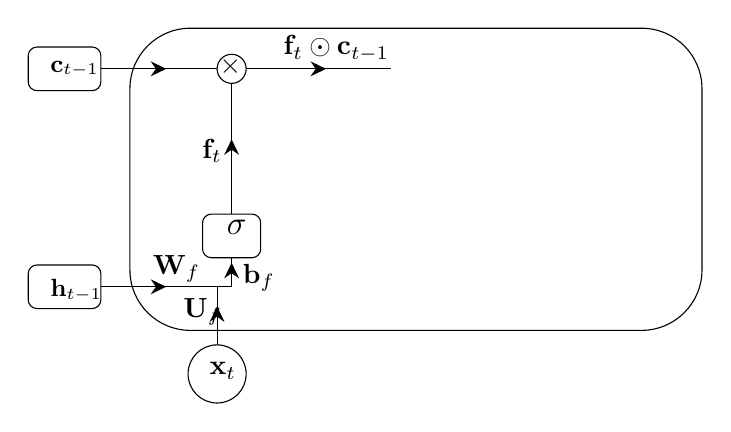
\begin{tikzpicture}[x=0.75pt,y=0.75pt,yscale=-0.7,xscale=0.7]
          %Shape: Ellipse [id:dp4969327327172295] 
          \draw   (160,280) .. controls (160,268.95) and (168.95,260) .. (180,260) .. controls (191.05,260) and (200,268.95) .. (200,280) .. controls (200,291.05) and (191.05,300) .. (180,300) .. controls (168.95,300) and (160,291.05) .. (160,280) -- cycle ;
          %Rounded Rect [id:dp8357991370192488] 
          \draw   (170,176) .. controls (170,172.69) and (172.69,170) .. (176,170) -- (204,170) .. controls (207.31,170) and (210,172.69) .. (210,176) -- (210,194) .. controls (210,197.31) and (207.31,200) .. (204,200) -- (176,200) .. controls (172.69,200) and (170,197.31) .. (170,194) -- cycle ;
          %Straight Lines [id:da3600219657240744] 
          \draw    (100,220) -- (180,220) ;
          \draw [shift={(145,220)}, rotate = 180] [fill={rgb, 255:red, 0; green, 0; blue, 0 }  ][line width=0.08]  [draw opacity=0] (10.72,-5.15) -- (0,0) -- (10.72,5.15) -- (7.12,0) -- cycle    ;
          %Rounded Rect [id:dp915587451603912] 
          \draw   (50,211) .. controls (50,207.69) and (52.69,205) .. (56,205) -- (94,205) .. controls (97.31,205) and (100,207.69) .. (100,211) -- (100,229) .. controls (100,232.31) and (97.31,235) .. (94,235) -- (56,235) .. controls (52.69,235) and (50,232.31) .. (50,229) -- cycle ;
          %Straight Lines [id:da9272238333173219] 
          \draw    (190,200) -- (190,220) ;
          \draw [shift={(190,203.5)}, rotate = 90] [fill={rgb, 255:red, 0; green, 0; blue, 0 }  ][line width=0.08]  [draw opacity=0] (10.72,-5.15) -- (0,0) -- (10.72,5.15) -- (7.12,0) -- cycle    ;
          %Straight Lines [id:da7830623178958898] 
          \draw    (190,80) -- (190,170) ;
          \draw [shift={(190,118.5)}, rotate = 90] [fill={rgb, 255:red, 0; green, 0; blue, 0 }  ][line width=0.08]  [draw opacity=0] (10.72,-5.15) -- (0,0) -- (10.72,5.15) -- (7.12,0) -- cycle    ;
          %Straight Lines [id:da008261007079938487] 
          \draw    (180,220) -- (180,260) ;
          \draw [shift={(180,233.5)}, rotate = 90] [fill={rgb, 255:red, 0; green, 0; blue, 0 }  ][line width=0.08]  [draw opacity=0] (10.72,-5.15) -- (0,0) -- (10.72,5.15) -- (7.12,0) -- cycle    ;
          %Straight Lines [id:da6327623101696669] 
          \draw    (180,220) -- (190,220) ;
          %Rounded Rect [id:dp1558027289731856] 
          \draw   (120,83.64) .. controls (120,60.67) and (138.62,42.05) .. (161.59,42.05) -- (472.14,42.05) .. controls (495.11,42.05) and (513.73,60.67) .. (513.73,83.64) -- (513.73,208.41) .. controls (513.73,231.38) and (495.11,250) .. (472.14,250) -- (161.59,250) .. controls (138.62,250) and (120,231.38) .. (120,208.41) -- cycle ;
          %Rounded Rect [id:dp3095760028615271] 
          \draw   (50,61) .. controls (50,57.69) and (52.69,55) .. (56,55) -- (94,55) .. controls (97.31,55) and (100,57.69) .. (100,61) -- (100,79) .. controls (100,82.31) and (97.31,85) .. (94,85) -- (56,85) .. controls (52.69,85) and (50,82.31) .. (50,79) -- cycle ;
          %Shape: Ellipse [id:dp04583613718786217] 
          \draw   (180,70) .. controls (180,64.48) and (184.48,60) .. (190,60) .. controls (195.52,60) and (200,64.48) .. (200,70) .. controls (200,75.52) and (195.52,80) .. (190,80) .. controls (184.48,80) and (180,75.52) .. (180,70) -- cycle ;
          %Straight Lines [id:da7337073083902665] 
          \draw    (100,70) -- (180,70) ;
          \draw [shift={(145,70)}, rotate = 180] [fill={rgb, 255:red, 0; green, 0; blue, 0 }  ][line width=0.08]  [draw opacity=0] (10.72,-5.15) -- (0,0) -- (10.72,5.15) -- (7.12,0) -- cycle    ;
          %Straight Lines [id:da19524926020736277] 
          \draw    (200,70) -- (300,70) ;
          \draw [shift={(255,70)}, rotate = 180] [fill={rgb, 255:red, 0; green, 0; blue, 0 }  ][line width=0.08]  [draw opacity=0] (10.72,-5.15) -- (0,0) -- (10.72,5.15) -- (7.12,0) -- cycle    ;

          % Text Node
          \draw (173,270.4) node [anchor=north west][inner sep=0.75pt]  [font=\normalsize]  {$\mathbf{x}_{t}$};
          % Text Node
          \draw (185,172.4) node [anchor=north west][inner sep=0.75pt]  [font=\large]  {$\boldsymbol{\sigma }$};
          % Text Node
          \draw (63.38,212.9) node [anchor=north west][inner sep=0.75pt]  [font=\small]  {$\mathbf{h}_{t-1}$};
          % Text Node
          \draw (168,116.4) node [anchor=north west][inner sep=0.75pt]  [font=\normalsize]  {$\mathbf{f}_{t}$};
          % Text Node
          \draw (224,45.4) node [anchor=north west][inner sep=0.75pt]  [font=\normalsize]  {$\mathbf{f}_{t} \odot \mathbf{c}_{t-1}$};
          % Text Node
          \draw (134,196.4) node [anchor=north west][inner sep=0.75pt]  [font=\normalsize]  {$\mathbf{W}_{f}$};
          % Text Node
          \draw (155,226.4) node [anchor=north west][inner sep=0.75pt]  [font=\normalsize]  {$\mathbf{U}_{f}$};
          % Text Node
          \draw (196,202.4) node [anchor=north west][inner sep=0.75pt]  [font=\normalsize]  {$\mathbf{b}_{f}$};
          % Text Node
          \draw (63.38,62.9) node [anchor=north west][inner sep=0.75pt]  [font=\small]  {$\mathbf{c}_{t-1}$};
          % Text Node
          \draw (180,60.4) node [anchor=north west][inner sep=0.75pt]  [font=\normalsize]  {$\times $};
        \end{tikzpicture}
        \caption{} 
        \label{fig:lstm_node_1}
      \end{figure}
      
      \item The \textbf{input gate} (denoted by $\mathbf{i}$) consists of two activations with the following operations. 
      \begin{align}
          \mathbf{i}_t & = \boldsymbol{\sigma}( \mathbf{W}_i \mathbf{h}_{t-1} + \mathbf{U}_i \mathbf{x}_t + \mathbf{b}_i ) \\
          \Tilde{\mathbf{c}}_t & = \boldsymbol{\tanh}( \mathbf{W}_c \mathbf{h}_{t-1} + \mathbf{U}_c \mathbf{x}_t + \mathbf{b}_c ) \\ 
          \mathbf{c}_t & = \mathbf{f}_t \odot \mathbf{c}_{t-1} + \mathbf{i}_t \odot \Tilde{\mathbf{c}}_t 
      \end{align}

      The layer $\mathbf{i}$ can be seen as the filter that selects which information can pass through it and what information to be discarded. To create this layer, we pass the short-term memory and current input into a sigmoid function, which will transform the values to be between $0$ and $1$, indicating which information is unimportant. The second layer $\Tilde{\mathbf{c}}$ takes the short term memory and current input and uses the $\tanh$ to transform the elements to be in $(-1, 1)$, which allows us to add or subtract the necessary information from the long term memory. 

      \begin{figure}[H]
        \centering 
        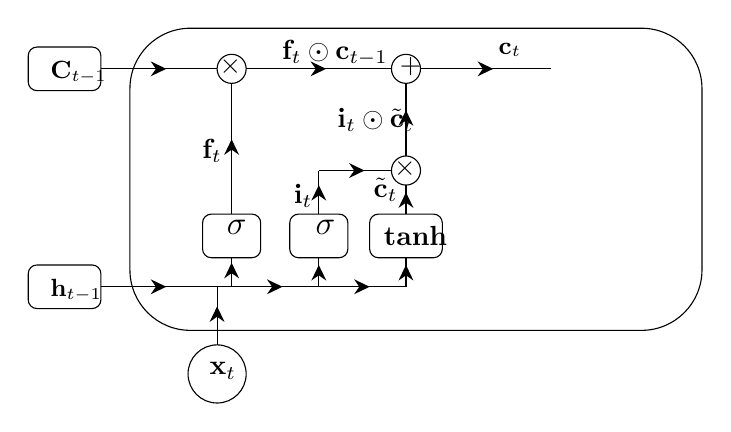
\begin{tikzpicture}[x=0.75pt,y=0.75pt,yscale=-0.7,xscale=0.7]
          %Shape: Ellipse [id:dp673856687206376] 
          \draw   (180,327.95) .. controls (180,316.91) and (188.95,307.95) .. (200,307.95) .. controls (211.05,307.95) and (220,316.91) .. (220,327.95) .. controls (220,339) and (211.05,347.95) .. (200,347.95) .. controls (188.95,347.95) and (180,339) .. (180,327.95) -- cycle ;
          %Rounded Rect [id:dp10309162377764869] 
          \draw   (190,223.95) .. controls (190,220.64) and (192.69,217.95) .. (196,217.95) -- (224,217.95) .. controls (227.31,217.95) and (230,220.64) .. (230,223.95) -- (230,241.95) .. controls (230,245.27) and (227.31,247.95) .. (224,247.95) -- (196,247.95) .. controls (192.69,247.95) and (190,245.27) .. (190,241.95) -- cycle ;
          %Straight Lines [id:da6240205957335716] 
          \draw    (120,267.95) -- (200,267.95) ;
          \draw [shift={(165,267.95)}, rotate = 180] [fill={rgb, 255:red, 0; green, 0; blue, 0 }  ][line width=0.08]  [draw opacity=0] (10.72,-5.15) -- (0,0) -- (10.72,5.15) -- (7.12,0) -- cycle    ;
          %Rounded Rect [id:dp6098888041343062] 
          \draw   (70,258.95) .. controls (70,255.64) and (72.69,252.95) .. (76,252.95) -- (114,252.95) .. controls (117.31,252.95) and (120,255.64) .. (120,258.95) -- (120,276.95) .. controls (120,280.27) and (117.31,282.95) .. (114,282.95) -- (76,282.95) .. controls (72.69,282.95) and (70,280.27) .. (70,276.95) -- cycle ;
          %Straight Lines [id:da6043978269854642] 
          \draw    (210,247.95) -- (210,267.95) ;
          \draw [shift={(210,251.45)}, rotate = 90] [fill={rgb, 255:red, 0; green, 0; blue, 0 }  ][line width=0.08]  [draw opacity=0] (10.72,-5.15) -- (0,0) -- (10.72,5.15) -- (7.12,0) -- cycle    ;
          %Straight Lines [id:da09325682821607639] 
          \draw    (210,127.95) -- (210,217.95) ;
          \draw [shift={(210,166.45)}, rotate = 90] [fill={rgb, 255:red, 0; green, 0; blue, 0 }  ][line width=0.08]  [draw opacity=0] (10.72,-5.15) -- (0,0) -- (10.72,5.15) -- (7.12,0) -- cycle    ;
          %Rounded Rect [id:dp605422940907552] 
          \draw   (250,223.95) .. controls (250,220.64) and (252.69,217.95) .. (256,217.95) -- (284,217.95) .. controls (287.31,217.95) and (290,220.64) .. (290,223.95) -- (290,241.95) .. controls (290,245.27) and (287.31,247.95) .. (284,247.95) -- (256,247.95) .. controls (252.69,247.95) and (250,245.27) .. (250,241.95) -- cycle ;
          %Straight Lines [id:da1280805304517283] 
          \draw    (200,267.95) -- (200,307.95) ;
          \draw [shift={(200,281.45)}, rotate = 90] [fill={rgb, 255:red, 0; green, 0; blue, 0 }  ][line width=0.08]  [draw opacity=0] (10.72,-5.15) -- (0,0) -- (10.72,5.15) -- (7.12,0) -- cycle    ;
          %Straight Lines [id:da34447299041881574] 
          \draw    (200,267.95) -- (210,267.95) ;
          %Straight Lines [id:da337875745538847] 
          \draw    (210,267.95) -- (270,267.95) ;
          \draw [shift={(245,267.95)}, rotate = 180] [fill={rgb, 255:red, 0; green, 0; blue, 0 }  ][line width=0.08]  [draw opacity=0] (10.72,-5.15) -- (0,0) -- (10.72,5.15) -- (7.12,0) -- cycle    ;
          %Rounded Rect [id:dp015328935957077405] 
          \draw   (305,223.95) .. controls (305,220.64) and (307.69,217.95) .. (311,217.95) -- (349,217.95) .. controls (352.31,217.95) and (355,220.64) .. (355,223.95) -- (355,241.95) .. controls (355,245.27) and (352.31,247.95) .. (349,247.95) -- (311,247.95) .. controls (307.69,247.95) and (305,245.27) .. (305,241.95) -- cycle ;
          %Straight Lines [id:da225547149220509] 
          \draw    (270,267.95) -- (270,247.95) ;
          \draw [shift={(270,252.95)}, rotate = 90] [fill={rgb, 255:red, 0; green, 0; blue, 0 }  ][line width=0.08]  [draw opacity=0] (10.72,-5.15) -- (0,0) -- (10.72,5.15) -- (7.12,0) -- cycle    ;
          %Straight Lines [id:da6795943289184077] 
          \draw    (330,267.95) -- (330,247.95) ;
          \draw [shift={(330,252.95)}, rotate = 90] [fill={rgb, 255:red, 0; green, 0; blue, 0 }  ][line width=0.08]  [draw opacity=0] (10.72,-5.15) -- (0,0) -- (10.72,5.15) -- (7.12,0) -- cycle    ;
          %Straight Lines [id:da21779293195502758] 
          \draw    (330,217.95) -- (330,197.95) ;
          \draw [shift={(330,202.95)}, rotate = 90] [fill={rgb, 255:red, 0; green, 0; blue, 0 }  ][line width=0.08]  [draw opacity=0] (10.72,-5.15) -- (0,0) -- (10.72,5.15) -- (7.12,0) -- cycle    ;
          %Straight Lines [id:da4764731211730844] 
          \draw    (270,217.95) -- (270,187.95) ;
          \draw [shift={(270,197.95)}, rotate = 90] [fill={rgb, 255:red, 0; green, 0; blue, 0 }  ][line width=0.08]  [draw opacity=0] (10.72,-5.15) -- (0,0) -- (10.72,5.15) -- (7.12,0) -- cycle    ;
          %Shape: Ellipse [id:dp38154006355076087] 
          \draw   (320,187.95) .. controls (320,182.43) and (324.48,177.95) .. (330,177.95) .. controls (335.52,177.95) and (340,182.43) .. (340,187.95) .. controls (340,193.48) and (335.52,197.95) .. (330,197.95) .. controls (324.48,197.95) and (320,193.48) .. (320,187.95) -- cycle ;
          %Straight Lines [id:da3258632871225313] 
          \draw    (320,187.95) -- (270,187.95) ;
          \draw [shift={(301.5,187.95)}, rotate = 180] [fill={rgb, 255:red, 0; green, 0; blue, 0 }  ][line width=0.08]  [draw opacity=0] (10.72,-5.15) -- (0,0) -- (10.72,5.15) -- (7.12,0) -- cycle    ;
          %Straight Lines [id:da5423947396221587] 
          \draw    (330,127.95) -- (330,177.95) ;
          \draw [shift={(330,146.45)}, rotate = 90] [fill={rgb, 255:red, 0; green, 0; blue, 0 }  ][line width=0.08]  [draw opacity=0] (10.72,-5.15) -- (0,0) -- (10.72,5.15) -- (7.12,0) -- cycle    ;
          %Straight Lines [id:da7595203590607811] 
          \draw    (270,267.95) -- (330,267.95) ;
          \draw [shift={(305,267.95)}, rotate = 180] [fill={rgb, 255:red, 0; green, 0; blue, 0 }  ][line width=0.08]  [draw opacity=0] (10.72,-5.15) -- (0,0) -- (10.72,5.15) -- (7.12,0) -- cycle    ;
          %Rounded Rect [id:dp998433719384372] 
          \draw   (140,131.59) .. controls (140,108.62) and (158.62,90) .. (181.59,90) -- (492.14,90) .. controls (515.11,90) and (533.73,108.62) .. (533.73,131.59) -- (533.73,256.36) .. controls (533.73,279.33) and (515.11,297.95) .. (492.14,297.95) -- (181.59,297.95) .. controls (158.62,297.95) and (140,279.33) .. (140,256.36) -- cycle ;
          %Rounded Rect [id:dp5009767130679297] 
          \draw   (70,108.95) .. controls (70,105.64) and (72.69,102.95) .. (76,102.95) -- (114,102.95) .. controls (117.31,102.95) and (120,105.64) .. (120,108.95) -- (120,126.95) .. controls (120,130.27) and (117.31,132.95) .. (114,132.95) -- (76,132.95) .. controls (72.69,132.95) and (70,130.27) .. (70,126.95) -- cycle ;
          %Shape: Ellipse [id:dp5406765889795262] 
          \draw   (200,117.95) .. controls (200,112.43) and (204.48,107.95) .. (210,107.95) .. controls (215.52,107.95) and (220,112.43) .. (220,117.95) .. controls (220,123.48) and (215.52,127.95) .. (210,127.95) .. controls (204.48,127.95) and (200,123.48) .. (200,117.95) -- cycle ;
          %Straight Lines [id:da2940801686510699] 
          \draw    (120,117.95) -- (200,117.95) ;
          \draw [shift={(165,117.95)}, rotate = 180] [fill={rgb, 255:red, 0; green, 0; blue, 0 }  ][line width=0.08]  [draw opacity=0] (10.72,-5.15) -- (0,0) -- (10.72,5.15) -- (7.12,0) -- cycle    ;
          %Straight Lines [id:da047556376575517145] 
          \draw    (220,117.95) -- (320,117.95) ;
          \draw [shift={(275,117.95)}, rotate = 180] [fill={rgb, 255:red, 0; green, 0; blue, 0 }  ][line width=0.08]  [draw opacity=0] (10.72,-5.15) -- (0,0) -- (10.72,5.15) -- (7.12,0) -- cycle    ;
          %Shape: Ellipse [id:dp004236969372855448] 
          \draw   (320,117.95) .. controls (320,112.43) and (324.48,107.95) .. (330,107.95) .. controls (335.52,107.95) and (340,112.43) .. (340,117.95) .. controls (340,123.48) and (335.52,127.95) .. (330,127.95) .. controls (324.48,127.95) and (320,123.48) .. (320,117.95) -- cycle ;
          %Straight Lines [id:da42944638467678886] 
          \draw    (340,117.95) -- (430,117.95) ;
          \draw [shift={(390,117.95)}, rotate = 180] [fill={rgb, 255:red, 0; green, 0; blue, 0 }  ][line width=0.08]  [draw opacity=0] (10.72,-5.15) -- (0,0) -- (10.72,5.15) -- (7.12,0) -- cycle    ;

          % Text Node
          \draw (193,318.35) node [anchor=north west][inner sep=0.75pt]  [font=\normalsize]  {$\mathbf{x}_{t}$};
          % Text Node
          \draw (205,220.35) node [anchor=north west][inner sep=0.75pt]  [font=\large]  {$\boldsymbol{\sigma }$};
          % Text Node
          \draw (83.38,260.85) node [anchor=north west][inner sep=0.75pt]  [font=\small]  {$\mathbf{h}_{t-1}$};
          % Text Node
          \draw (266,220.35) node [anchor=north west][inner sep=0.75pt]  [font=\large]  {$\boldsymbol{\sigma }$};
          % Text Node
          \draw (188,164.35) node [anchor=north west][inner sep=0.75pt]  [font=\normalsize]  {$\mathbf{f}_{t}$};
          % Text Node
          \draw (313,224.35) node [anchor=north west][inner sep=0.75pt]  [font=\normalsize]  {$\mathbf{tanh}$};
          % Text Node
          \draw (320,178.35) node [anchor=north west][inner sep=0.75pt]  [font=\normalsize]  {$\times $};
          % Text Node
          \draw (83.38,110.85) node [anchor=north west][inner sep=0.75pt]  [font=\small]  {$\mathbf{C}_{t-1}$};
          % Text Node
          \draw (200,108.35) node [anchor=north west][inner sep=0.75pt]  [font=\normalsize]  {$\times $};
          % Text Node
          \draw (324,108.35) node [anchor=north west][inner sep=0.75pt]  [font=\normalsize]  {$+$};
          % Text Node
          \draw (251,195.4) node [anchor=north west][inner sep=0.75pt]  [font=\normalsize]  {$\mathbf{i}_{t}$};
          % Text Node
          \draw (306,191.4) node [anchor=north west][inner sep=0.75pt]  [font=\normalsize]  {$\tilde{\mathbf{c}}_{t}$};
          % Text Node
          \draw (243,96.4) node [anchor=north west][inner sep=0.75pt]  [font=\normalsize]  {$\mathbf{f}_{t} \odot \mathbf{c}_{t-1}$};
          % Text Node
          \draw (281,143.4) node [anchor=north west][inner sep=0.75pt]  [font=\normalsize]  {$\mathbf{i}_{t} \odot \tilde{\mathbf{c}}_{t}$};
          % Text Node
          \draw (392,98.4) node [anchor=north west][inner sep=0.75pt]  [font=\small]  {$\mathbf{c}_{t}$};
        \end{tikzpicture}
        \caption{} 
        \label{fig:lstm_node_2}
      \end{figure}

      \item The \textbf{output gate} (denoted by $\mathbf{o}$) consists of two activations with the following operations. This again creates a separate filter that selects the relevant information needed for the short term memory. 
      \begin{align}
          \mathbf{o}_t & = \boldsymbol{\sigma}( \mathbf{W}_o \mathbf{h}_{t-1} + \mathbf{U}_o \mathbf{x}_t + \mathbf{b}_o ) \\
          \mathbf{h}_t & = \mathbf{o}_t \odot \boldsymbol{\tanh}(\mathbf{c}_t) \\
          \hat{\mathbf{y}}_t & = \boldsymbol{\sigma}_y ( \mathbf{V} \mathbf{h}_t + \mathbf{b}_y)
      \end{align}

      \begin{figure}[H]
        \centering 
        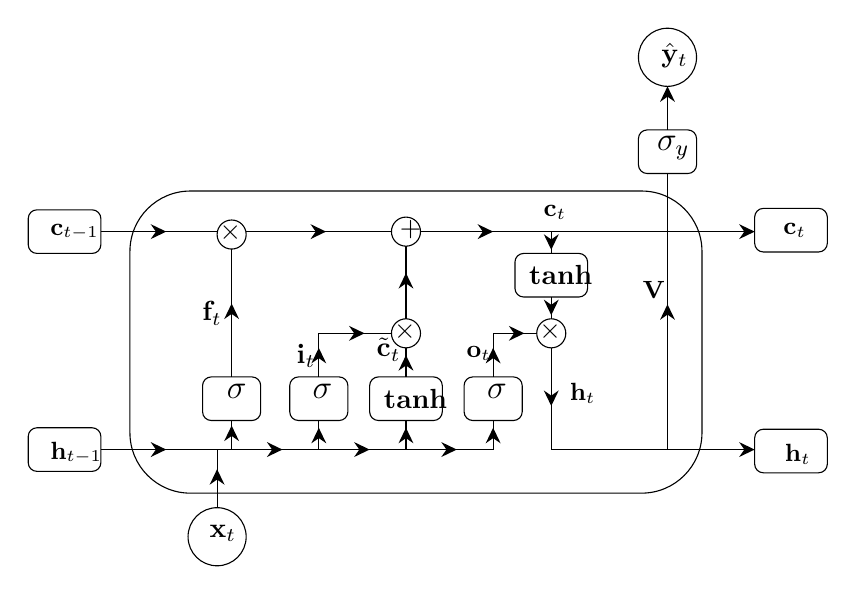
\begin{tikzpicture}[x=0.75pt,y=0.75pt,yscale=-0.7,xscale=0.7]
          %Rounded Rect [id:dp7607307729058677] 
          \draw   (140,163.64) .. controls (140,140.67) and (158.62,122.05) .. (181.59,122.05) -- (492.14,122.05) .. controls (515.11,122.05) and (533.73,140.67) .. (533.73,163.64) -- (533.73,288.41) .. controls (533.73,311.38) and (515.11,330) .. (492.14,330) -- (181.59,330) .. controls (158.62,330) and (140,311.38) .. (140,288.41) -- cycle ;
          %Shape: Ellipse [id:dp900217564752672] 
          \draw   (180,360) .. controls (180,348.95) and (188.95,340) .. (200,340) .. controls (211.05,340) and (220,348.95) .. (220,360) .. controls (220,371.05) and (211.05,380) .. (200,380) .. controls (188.95,380) and (180,371.05) .. (180,360) -- cycle ;
          %Rounded Rect [id:dp6893065668366456] 
          \draw   (190,256) .. controls (190,252.69) and (192.69,250) .. (196,250) -- (224,250) .. controls (227.31,250) and (230,252.69) .. (230,256) -- (230,274) .. controls (230,277.31) and (227.31,280) .. (224,280) -- (196,280) .. controls (192.69,280) and (190,277.31) .. (190,274) -- cycle ;
          %Straight Lines [id:da5343888843478] 
          \draw    (120,300) -- (200,300) ;
          \draw [shift={(165,300)}, rotate = 180] [fill={rgb, 255:red, 0; green, 0; blue, 0 }  ][line width=0.08]  [draw opacity=0] (10.72,-5.15) -- (0,0) -- (10.72,5.15) -- (7.12,0) -- cycle    ;
          %Rounded Rect [id:dp16398311464764093] 
          \draw   (70,291) .. controls (70,287.69) and (72.69,285) .. (76,285) -- (114,285) .. controls (117.31,285) and (120,287.69) .. (120,291) -- (120,309) .. controls (120,312.31) and (117.31,315) .. (114,315) -- (76,315) .. controls (72.69,315) and (70,312.31) .. (70,309) -- cycle ;
          %Rounded Rect [id:dp7552509756915937] 
          \draw   (70,141) .. controls (70,137.69) and (72.69,135) .. (76,135) -- (114,135) .. controls (117.31,135) and (120,137.69) .. (120,141) -- (120,159) .. controls (120,162.31) and (117.31,165) .. (114,165) -- (76,165) .. controls (72.69,165) and (70,162.31) .. (70,159) -- cycle ;
          %Straight Lines [id:da304843264938752] 
          \draw    (210,280) -- (210,300) ;
          \draw [shift={(210,283.5)}, rotate = 90] [fill={rgb, 255:red, 0; green, 0; blue, 0 }  ][line width=0.08]  [draw opacity=0] (10.72,-5.15) -- (0,0) -- (10.72,5.15) -- (7.12,0) -- cycle    ;
          %Straight Lines [id:da14284118067632345] 
          \draw    (210,162) -- (210,250) ;
          \draw [shift={(210,199.5)}, rotate = 90] [fill={rgb, 255:red, 0; green, 0; blue, 0 }  ][line width=0.08]  [draw opacity=0] (10.72,-5.15) -- (0,0) -- (10.72,5.15) -- (7.12,0) -- cycle    ;
          %Shape: Ellipse [id:dp5396089408185574] 
          \draw   (200,152) .. controls (200,146.48) and (204.48,142) .. (210,142) .. controls (215.52,142) and (220,146.48) .. (220,152) .. controls (220,157.52) and (215.52,162) .. (210,162) .. controls (204.48,162) and (200,157.52) .. (200,152) -- cycle ;
          %Straight Lines [id:da9933430333496693] 
          \draw    (120,150) -- (200,150) ;
          \draw [shift={(165,150)}, rotate = 180] [fill={rgb, 255:red, 0; green, 0; blue, 0 }  ][line width=0.08]  [draw opacity=0] (10.72,-5.15) -- (0,0) -- (10.72,5.15) -- (7.12,0) -- cycle    ;
          %Straight Lines [id:da8940095383250102] 
          \draw    (220,150) -- (320,150) ;
          \draw [shift={(275,150)}, rotate = 180] [fill={rgb, 255:red, 0; green, 0; blue, 0 }  ][line width=0.08]  [draw opacity=0] (10.72,-5.15) -- (0,0) -- (10.72,5.15) -- (7.12,0) -- cycle    ;
          %Rounded Rect [id:dp25314537917502555] 
          \draw   (250,256) .. controls (250,252.69) and (252.69,250) .. (256,250) -- (284,250) .. controls (287.31,250) and (290,252.69) .. (290,256) -- (290,274) .. controls (290,277.31) and (287.31,280) .. (284,280) -- (256,280) .. controls (252.69,280) and (250,277.31) .. (250,274) -- cycle ;
          %Straight Lines [id:da7871629509904587] 
          \draw    (200,300) -- (200,340) ;
          \draw [shift={(200,313.5)}, rotate = 90] [fill={rgb, 255:red, 0; green, 0; blue, 0 }  ][line width=0.08]  [draw opacity=0] (10.72,-5.15) -- (0,0) -- (10.72,5.15) -- (7.12,0) -- cycle    ;
          %Straight Lines [id:da1940620806488591] 
          \draw    (200,300) -- (210,300) ;
          %Straight Lines [id:da5912482065359186] 
          \draw    (210,300) -- (270,300) ;
          \draw [shift={(245,300)}, rotate = 180] [fill={rgb, 255:red, 0; green, 0; blue, 0 }  ][line width=0.08]  [draw opacity=0] (10.72,-5.15) -- (0,0) -- (10.72,5.15) -- (7.12,0) -- cycle    ;
          %Shape: Ellipse [id:dp4841686324219643] 
          \draw   (320,150) .. controls (320,144.48) and (324.48,140) .. (330,140) .. controls (335.52,140) and (340,144.48) .. (340,150) .. controls (340,155.52) and (335.52,160) .. (330,160) .. controls (324.48,160) and (320,155.52) .. (320,150) -- cycle ;
          %Rounded Rect [id:dp31865438690386094] 
          \draw   (305,256) .. controls (305,252.69) and (307.69,250) .. (311,250) -- (349,250) .. controls (352.31,250) and (355,252.69) .. (355,256) -- (355,274) .. controls (355,277.31) and (352.31,280) .. (349,280) -- (311,280) .. controls (307.69,280) and (305,277.31) .. (305,274) -- cycle ;
          %Straight Lines [id:da5645041143915148] 
          \draw    (270,300) -- (270,280) ;
          \draw [shift={(270,285)}, rotate = 90] [fill={rgb, 255:red, 0; green, 0; blue, 0 }  ][line width=0.08]  [draw opacity=0] (10.72,-5.15) -- (0,0) -- (10.72,5.15) -- (7.12,0) -- cycle    ;
          %Straight Lines [id:da9431818949019313] 
          \draw    (330,300) -- (330,280) ;
          \draw [shift={(330,285)}, rotate = 90] [fill={rgb, 255:red, 0; green, 0; blue, 0 }  ][line width=0.08]  [draw opacity=0] (10.72,-5.15) -- (0,0) -- (10.72,5.15) -- (7.12,0) -- cycle    ;
          %Straight Lines [id:da11777621499218438] 
          \draw    (330,250) -- (330,230) ;
          \draw [shift={(330,235)}, rotate = 90] [fill={rgb, 255:red, 0; green, 0; blue, 0 }  ][line width=0.08]  [draw opacity=0] (10.72,-5.15) -- (0,0) -- (10.72,5.15) -- (7.12,0) -- cycle    ;
          %Straight Lines [id:da9724379887976446] 
          \draw    (270,250) -- (270,220) ;
          \draw [shift={(270,230)}, rotate = 90] [fill={rgb, 255:red, 0; green, 0; blue, 0 }  ][line width=0.08]  [draw opacity=0] (10.72,-5.15) -- (0,0) -- (10.72,5.15) -- (7.12,0) -- cycle    ;
          %Shape: Ellipse [id:dp6921024732199978] 
          \draw   (320,220) .. controls (320,214.48) and (324.48,210) .. (330,210) .. controls (335.52,210) and (340,214.48) .. (340,220) .. controls (340,225.52) and (335.52,230) .. (330,230) .. controls (324.48,230) and (320,225.52) .. (320,220) -- cycle ;
          %Straight Lines [id:da1410394226097551] 
          \draw    (320,220) -- (270,220) ;
          \draw [shift={(301.5,220)}, rotate = 180] [fill={rgb, 255:red, 0; green, 0; blue, 0 }  ][line width=0.08]  [draw opacity=0] (10.72,-5.15) -- (0,0) -- (10.72,5.15) -- (7.12,0) -- cycle    ;
          %Straight Lines [id:da4451936356762698] 
          \draw    (330,160) -- (330,210) ;
          \draw [shift={(330,178.5)}, rotate = 90] [fill={rgb, 255:red, 0; green, 0; blue, 0 }  ][line width=0.08]  [draw opacity=0] (10.72,-5.15) -- (0,0) -- (10.72,5.15) -- (7.12,0) -- cycle    ;
          %Straight Lines [id:da8250107200889327] 
          \draw    (270,300) -- (330,300) ;
          \draw [shift={(305,300)}, rotate = 180] [fill={rgb, 255:red, 0; green, 0; blue, 0 }  ][line width=0.08]  [draw opacity=0] (10.72,-5.15) -- (0,0) -- (10.72,5.15) -- (7.12,0) -- cycle    ;
          %Straight Lines [id:da31368624536525] 
          \draw    (340,150) -- (430,150) ;
          \draw [shift={(390,150)}, rotate = 180] [fill={rgb, 255:red, 0; green, 0; blue, 0 }  ][line width=0.08]  [draw opacity=0] (10.72,-5.15) -- (0,0) -- (10.72,5.15) -- (7.12,0) -- cycle    ;
          %Straight Lines [id:da680791431454264] 
          \draw    (330,300) -- (390,300) ;
          \draw [shift={(365,300)}, rotate = 180] [fill={rgb, 255:red, 0; green, 0; blue, 0 }  ][line width=0.08]  [draw opacity=0] (10.72,-5.15) -- (0,0) -- (10.72,5.15) -- (7.12,0) -- cycle    ;
          %Rounded Rect [id:dp4093507732748505] 
          \draw   (370,256) .. controls (370,252.69) and (372.69,250) .. (376,250) -- (404,250) .. controls (407.31,250) and (410,252.69) .. (410,256) -- (410,274) .. controls (410,277.31) and (407.31,280) .. (404,280) -- (376,280) .. controls (372.69,280) and (370,277.31) .. (370,274) -- cycle ;
          %Straight Lines [id:da05493337879481186] 
          \draw    (390,300) -- (390,280) ;
          \draw [shift={(390,285)}, rotate = 90] [fill={rgb, 255:red, 0; green, 0; blue, 0 }  ][line width=0.08]  [draw opacity=0] (10.72,-5.15) -- (0,0) -- (10.72,5.15) -- (7.12,0) -- cycle    ;
          %Straight Lines [id:da2852801639207645] 
          \draw    (390,250) -- (390,220) ;
          \draw [shift={(390,230)}, rotate = 90] [fill={rgb, 255:red, 0; green, 0; blue, 0 }  ][line width=0.08]  [draw opacity=0] (10.72,-5.15) -- (0,0) -- (10.72,5.15) -- (7.12,0) -- cycle    ;
          %Straight Lines [id:da10205317474403763] 
          \draw    (420,220) -- (390,220) ;
          \draw [shift={(411.5,220)}, rotate = 180] [fill={rgb, 255:red, 0; green, 0; blue, 0 }  ][line width=0.08]  [draw opacity=0] (10.72,-5.15) -- (0,0) -- (10.72,5.15) -- (7.12,0) -- cycle    ;
          %Shape: Ellipse [id:dp656470469132832] 
          \draw   (420,220) .. controls (420,214.48) and (424.48,210) .. (430,210) .. controls (435.52,210) and (440,214.48) .. (440,220) .. controls (440,225.52) and (435.52,230) .. (430,230) .. controls (424.48,230) and (420,225.52) .. (420,220) -- cycle ;
          %Rounded Rect [id:dp7702057134779456] 
          \draw   (405,171) .. controls (405,167.69) and (407.69,165) .. (411,165) -- (449,165) .. controls (452.31,165) and (455,167.69) .. (455,171) -- (455,189) .. controls (455,192.31) and (452.31,195) .. (449,195) -- (411,195) .. controls (407.69,195) and (405,192.31) .. (405,189) -- cycle ;
          %Straight Lines [id:da06612853990545564] 
          \draw    (430,150) -- (430,165) ;
          \draw [shift={(430,162.5)}, rotate = 270] [fill={rgb, 255:red, 0; green, 0; blue, 0 }  ][line width=0.08]  [draw opacity=0] (10.72,-5.15) -- (0,0) -- (10.72,5.15) -- (7.12,0) -- cycle    ;
          %Straight Lines [id:da9855082148874492] 
          \draw    (430,195) -- (430,210) ;
          \draw [shift={(430,207.5)}, rotate = 270] [fill={rgb, 255:red, 0; green, 0; blue, 0 }  ][line width=0.08]  [draw opacity=0] (10.72,-5.15) -- (0,0) -- (10.72,5.15) -- (7.12,0) -- cycle    ;
          %Straight Lines [id:da6917168175796875] 
          \draw    (430,150) -- (567,150) ;
          \draw [shift={(570,150)}, rotate = 180] [fill={rgb, 255:red, 0; green, 0; blue, 0 }  ][line width=0.08]  [draw opacity=0] (10.72,-5.15) -- (0,0) -- (10.72,5.15) -- (7.12,0) -- cycle    ;
          %Rounded Rect [id:dp7717143285394976] 
          \draw   (570,140) .. controls (570,136.69) and (572.69,134) .. (576,134) -- (614,134) .. controls (617.31,134) and (620,136.69) .. (620,140) -- (620,158) .. controls (620,161.31) and (617.31,164) .. (614,164) -- (576,164) .. controls (572.69,164) and (570,161.31) .. (570,158) -- cycle ;
          %Straight Lines [id:da9058130105060662] 
          \draw    (430,230) -- (430,300) ;
          \draw [shift={(430,270)}, rotate = 270] [fill={rgb, 255:red, 0; green, 0; blue, 0 }  ][line width=0.08]  [draw opacity=0] (10.72,-5.15) -- (0,0) -- (10.72,5.15) -- (7.12,0) -- cycle    ;
          %Straight Lines [id:da40006208395694376] 
          \draw    (430,300) -- (567,300) ;
          \draw [shift={(570,300)}, rotate = 180] [fill={rgb, 255:red, 0; green, 0; blue, 0 }  ][line width=0.08]  [draw opacity=0] (10.72,-5.15) -- (0,0) -- (10.72,5.15) -- (7.12,0) -- cycle    ;
          %Rounded Rect [id:dp8925711851370559] 
          \draw   (570,292) .. controls (570,288.69) and (572.69,286) .. (576,286) -- (614,286) .. controls (617.31,286) and (620,288.69) .. (620,292) -- (620,310) .. controls (620,313.31) and (617.31,316) .. (614,316) -- (576,316) .. controls (572.69,316) and (570,313.31) .. (570,310) -- cycle ;
          %Straight Lines [id:da3431993487488634] 
          \draw    (510,300) -- (510,110) ;
          \draw [shift={(510,200)}, rotate = 90] [fill={rgb, 255:red, 0; green, 0; blue, 0 }  ][line width=0.08]  [draw opacity=0] (10.72,-5.15) -- (0,0) -- (10.72,5.15) -- (7.12,0) -- cycle    ;
          %Shape: Ellipse [id:dp5223810693241391] 
          \draw   (490,30) .. controls (490,18.95) and (498.95,10) .. (510,10) .. controls (521.05,10) and (530,18.95) .. (530,30) .. controls (530,41.05) and (521.05,50) .. (510,50) .. controls (498.95,50) and (490,41.05) .. (490,30) -- cycle ;
          %Rounded Rect [id:dp08850756436330398] 
          \draw   (490,86) .. controls (490,82.69) and (492.69,80) .. (496,80) -- (524,80) .. controls (527.31,80) and (530,82.69) .. (530,86) -- (530,104) .. controls (530,107.31) and (527.31,110) .. (524,110) -- (496,110) .. controls (492.69,110) and (490,107.31) .. (490,104) -- cycle ;
          %Straight Lines [id:da8380296553480746] 
          \draw    (510,80) -- (510,53) ;
          \draw [shift={(510,50)}, rotate = 90] [fill={rgb, 255:red, 0; green, 0; blue, 0 }  ][line width=0.08]  [draw opacity=0] (10.72,-5.15) -- (0,0) -- (10.72,5.15) -- (7.12,0) -- cycle    ;

          % Text Node
          \draw (193,350.4) node [anchor=north west][inner sep=0.75pt]  [font=\normalsize]  {$\mathbf{x}_{t}$};
          % Text Node
          \draw (205,253.4) node [anchor=north west][inner sep=0.75pt]  [font=\large]  {$\boldsymbol{\sigma }$};
          % Text Node
          \draw (83.38,292.9) node [anchor=north west][inner sep=0.75pt]  [font=\small]  {$\mathbf{h}_{t-1}$};
          % Text Node
          \draw (83.38,142.9) node [anchor=north west][inner sep=0.75pt]  [font=\small]  {$\mathbf{c}_{t-1}$};
          % Text Node
          \draw (200,142.4) node [anchor=north west][inner sep=0.75pt]  [font=\normalsize]  {$\times $};
          % Text Node
          \draw (264,253.4) node [anchor=north west][inner sep=0.75pt]  [font=\large]  {$\boldsymbol{\sigma }$};
          % Text Node
          \draw (188,196.4) node [anchor=north west][inner sep=0.75pt]  [font=\normalsize]  {$\mathbf{f}_{t}$};
          % Text Node
          \draw (324,140.4) node [anchor=north west][inner sep=0.75pt]  [font=\normalsize]  {$+$};
          % Text Node
          \draw (313,256.4) node [anchor=north west][inner sep=0.75pt]  [font=\normalsize]  {$\mathbf{tanh}$};
          % Text Node
          \draw (320,210.4) node [anchor=north west][inner sep=0.75pt]  [font=\normalsize]  {$\times $};
          % Text Node
          \draw (384,253.4) node [anchor=north west][inner sep=0.75pt]  [font=\large]  {$\boldsymbol{\sigma }$};
          % Text Node
          \draw (420,210.4) node [anchor=north west][inner sep=0.75pt]  [font=\normalsize]  {$\times $};
          % Text Node
          \draw (413,171.4) node [anchor=north west][inner sep=0.75pt]  [font=\normalsize]  {$\mathbf{tanh}$};
          % Text Node
          \draw (588,142.4) node [anchor=north west][inner sep=0.75pt]  [font=\small]  {$\mathbf{c}_{t}$};
          % Text Node
          \draw (589,294.4) node [anchor=north west][inner sep=0.75pt]  [font=\small]  {$\mathbf{h}_{t}$};
          % Text Node
          \draw (504,18.4) node [anchor=north west][inner sep=0.75pt]  [font=\normalsize]  {$\hat{\mathbf{y}}_{t}$};
          % Text Node
          \draw (423,130.4) node [anchor=north west][inner sep=0.75pt]  [font=\small]  {$\mathbf{c}_{t}$};
          % Text Node
          \draw (370,227.4) node [anchor=north west][inner sep=0.75pt]  [font=\small]  {$\mathbf{o}_{t}$};
          % Text Node
          \draw (441,252.4) node [anchor=north west][inner sep=0.75pt]  [font=\small]  {$\mathbf{h}_{t}$};
          % Text Node
          \draw (501,82.4) node [anchor=north west][inner sep=0.75pt]  [font=\large]  {$\boldsymbol{\sigma }_{y}$};
          % Text Node
          \draw (491,182.4) node [anchor=north west][inner sep=0.75pt]  [font=\small]  {$\mathbf{V}$};
          % Text Node
          \draw (253,225.4) node [anchor=north west][inner sep=0.75pt]  [font=\normalsize]  {$\mathbf{i}_{t}$};
          % Text Node
          \draw (308,221.4) node [anchor=north west][inner sep=0.75pt]  [font=\normalsize]  {$\tilde{\mathbf{c}}_{t}$};
        \end{tikzpicture}
        \caption{} 
        \label{fig:lstm_node_3}
      \end{figure}
  \end{enumerate}
  That is it! Now focusing on the cell state in the diagram above. Note that in order to go from cell state $\mathbf{c}_{t-1}$ to $\mathbf{c}_t$, there was not a whole lot done to it. We really just multiply it once, which potentially deletes some content, and add it once, which adds new content, and we are done. The magic is this addition, since unlike multiplication, which can result in an exponential decay of knowledge, you are just constantly adding new numbers to update the storage, allowing the cell state to behave much more like RAM of a computer. 

  The LSTM architecture also makes it easier for the RNN to preserve information over many timesteps. For example, if the forget gate $\mathbf{f}_t$ is set to $\mathbf{1}$ and the input gate set to $\mathbf{0}$, then the information of that cell is preserved indefinitely. In contrast, it's harder for a vanilla RNN to learn a recurrent weight matrix $\mathbf{W}$ that preserves information in the hidden state. In practice, a vanilla RNN would preserve memory up to maybe 7 timesteps (and increasing this is extremely difficult) while a LSTM would get about 100 timesteps, so in practice you should almost always just use a LSTM. 

  Unfortunately, LSTM doesn't \textit{guarantee} that there is no vanishing or exploding gradients, but it does provide an easier way for the model to learn long-distance dependencies. Note that the gradient problem is not just a problem for RNNs; any neural architecture (including a feed-forward or convolutional) with very deep layers with multiple compositions of functions may suffer. Due to the chain rule and choice of nonlinearity function, these gradients can become vanishingly small and lower layers are learned very slowly. However, we can still implement residual connections to allow for more gradient flow such as ResNet, DenseNet, and HighwayNet. 

  \subsubsection{Multilayer LSTMs}

    We can extend this architecture in the exactly same way for multilayer LSTMs. Note that we should be careful of the transformations each arrow represents. For the arrows going from $\mathbf{h}_{t}^{[l]} \mapsto \mathbf{h}_{t}^{[l+1]}$, there is no further transformation since we are just pushing this vector as an input to the next LSTM node. However, the arrow pushing from $\mathbf{c}_t^{[L]} \mapsto \hat{\mathbf{y}}_{t}$ does have an extra affine transformation with $\mathbf{V}$ and $\mathbf{b}_y$, followed by some link function $\boldsymbol{\sigma}_y$ before we have the true prediction.  

    \begin{figure}[H]
      \centering 
      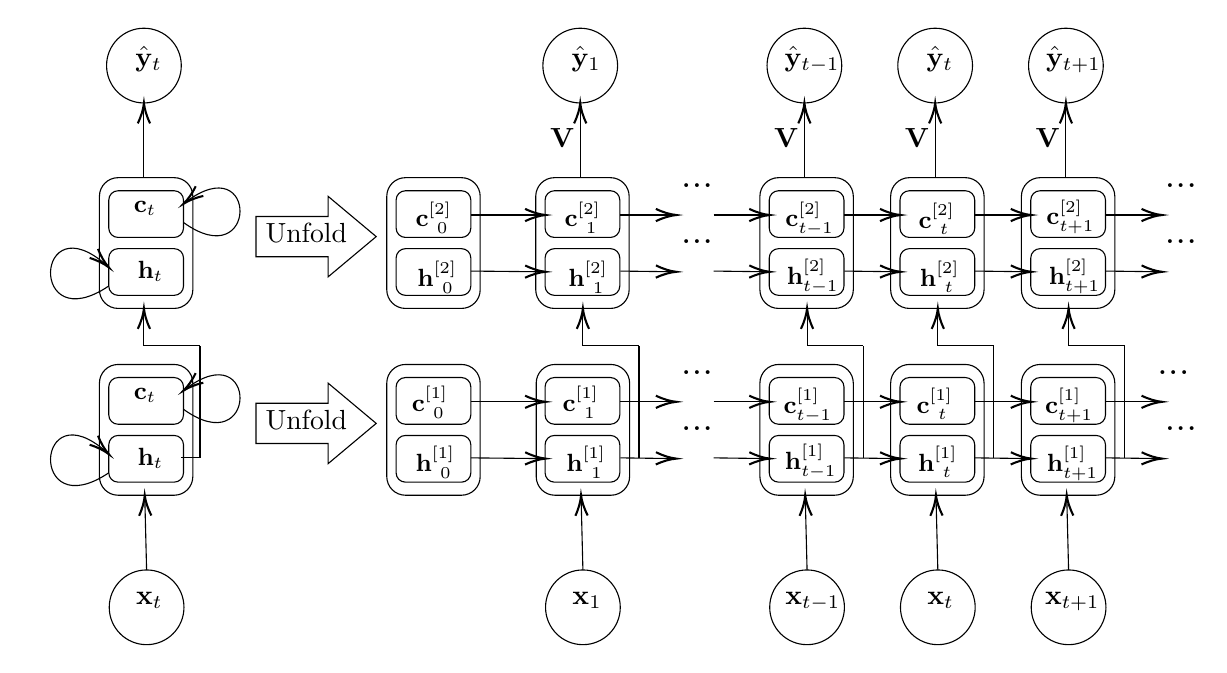
\begin{tikzpicture}[x=0.75pt,y=0.75pt,yscale=-0.9,xscale=0.9]
        %Rounded Rect [id:dp1729121626387391] 
        \draw   (51.18,200) .. controls (51.18,194.48) and (55.66,190) .. (61.18,190) -- (91.18,190) .. controls (96.71,190) and (101.18,194.48) .. (101.18,200) -- (101.18,250) .. controls (101.18,255.52) and (96.71,260) .. (91.18,260) -- (61.18,260) .. controls (55.66,260) and (51.18,255.52) .. (51.18,250) -- cycle ;
        %Rounded Rect [id:dp6162380210016798] 
        \draw   (56.18,202) .. controls (56.18,199.24) and (58.42,197) .. (61.18,197) -- (91.18,197) .. controls (93.95,197) and (96.18,199.24) .. (96.18,202) -- (96.18,217) .. controls (96.18,219.76) and (93.95,222) .. (91.18,222) -- (61.18,222) .. controls (58.42,222) and (56.18,219.76) .. (56.18,217) -- cycle ;
        %Rounded Rect [id:dp10367639876664736] 
        \draw   (56.18,233) .. controls (56.18,230.24) and (58.42,228) .. (61.18,228) -- (91.18,228) .. controls (93.95,228) and (96.18,230.24) .. (96.18,233) -- (96.18,248) .. controls (96.18,250.76) and (93.95,253) .. (91.18,253) -- (61.18,253) .. controls (58.42,253) and (56.18,250.76) .. (56.18,248) -- cycle ;
        %Curve Lines [id:da20240529841221622] 
        \draw [color={rgb, 255:red, 0; green, 0; blue, 0 }  ,draw opacity=1 ]   (96.18,214) .. controls (136.11,242.71) and (136.51,173.41) .. (97.38,203.07) ;
        \draw [shift={(96.18,204)}, rotate = 321.57] [color={rgb, 255:red, 0; green, 0; blue, 0 }  ,draw opacity=1 ][line width=0.75]    (10.93,-3.29) .. controls (6.95,-1.4) and (3.31,-0.3) .. (0,0) .. controls (3.31,0.3) and (6.95,1.4) .. (10.93,3.29)   ;
        %Curve Lines [id:da631199065967021] 
        \draw [color={rgb, 255:red, 0; green, 0; blue, 0 }  ,draw opacity=1 ]   (56.18,248) .. controls (13.06,276.93) and (16.55,202.73) .. (55.01,236.93) ;
        \draw [shift={(56.18,238)}, rotate = 222.92] [color={rgb, 255:red, 0; green, 0; blue, 0 }  ,draw opacity=1 ][line width=0.75]    (10.93,-3.29) .. controls (6.95,-1.4) and (3.31,-0.3) .. (0,0) .. controls (3.31,0.3) and (6.95,1.4) .. (10.93,3.29)   ;
        %Shape: Ellipse [id:dp3395210228264245] 
        \draw   (55,30) .. controls (55,18.95) and (63.95,10) .. (75,10) .. controls (86.05,10) and (95,18.95) .. (95,30) .. controls (95,41.05) and (86.05,50) .. (75,50) .. controls (63.95,50) and (55,41.05) .. (55,30) -- cycle ;
        %Straight Lines [id:da17924855399151696] 
        \draw [color={rgb, 255:red, 0; green, 0; blue, 0 }  ,draw opacity=1 ]   (75,90) -- (75,56) -- (75,52) ;
        \draw [shift={(75,50)}, rotate = 90] [color={rgb, 255:red, 0; green, 0; blue, 0 }  ,draw opacity=1 ][line width=0.75]    (10.93,-3.29) .. controls (6.95,-1.4) and (3.31,-0.3) .. (0,0) .. controls (3.31,0.3) and (6.95,1.4) .. (10.93,3.29)   ;
        %Shape: Ellipse [id:dp35088397695352525] 
        \draw   (56.43,320) .. controls (56.43,308.95) and (65.39,300) .. (76.43,300) .. controls (87.48,300) and (96.43,308.95) .. (96.43,320) .. controls (96.43,331.05) and (87.48,340) .. (76.43,340) .. controls (65.39,340) and (56.43,331.05) .. (56.43,320) -- cycle ;
        %Straight Lines [id:da37668288702619046] 
        \draw [color={rgb, 255:red, 0; green, 0; blue, 0 }  ,draw opacity=1 ]   (76.43,300) -- (75.48,262) ;
        \draw [shift={(75.43,260)}, rotate = 88.57] [color={rgb, 255:red, 0; green, 0; blue, 0 }  ,draw opacity=1 ][line width=0.75]    (10.93,-3.29) .. controls (6.95,-1.4) and (3.31,-0.3) .. (0,0) .. controls (3.31,0.3) and (6.95,1.4) .. (10.93,3.29)   ;
        %Rounded Rect [id:dp6301942583699514] 
        \draw   (285,200) .. controls (285,194.48) and (289.48,190) .. (295,190) -- (325,190) .. controls (330.52,190) and (335,194.48) .. (335,200) -- (335,250) .. controls (335,255.52) and (330.52,260) .. (325,260) -- (295,260) .. controls (289.48,260) and (285,255.52) .. (285,250) -- cycle ;
        %Rounded Rect [id:dp13078032445732224] 
        \draw   (289.75,202) .. controls (289.75,199.24) and (291.99,197) .. (294.75,197) -- (324.75,197) .. controls (327.51,197) and (329.75,199.24) .. (329.75,202) -- (329.75,217) .. controls (329.75,219.76) and (327.51,222) .. (324.75,222) -- (294.75,222) .. controls (291.99,222) and (289.75,219.76) .. (289.75,217) -- cycle ;
        %Rounded Rect [id:dp8684919320431015] 
        \draw   (289.75,233) .. controls (289.75,230.24) and (291.99,228) .. (294.75,228) -- (324.75,228) .. controls (327.51,228) and (329.75,230.24) .. (329.75,233) -- (329.75,248) .. controls (329.75,250.76) and (327.51,253) .. (324.75,253) -- (294.75,253) .. controls (291.99,253) and (289.75,250.76) .. (289.75,248) -- cycle ;
        %Shape: Ellipse [id:dp7681939879104125] 
        \draw   (288.57,30) .. controls (288.57,18.95) and (297.52,10) .. (308.57,10) .. controls (319.61,10) and (328.57,18.95) .. (328.57,30) .. controls (328.57,41.05) and (319.61,50) .. (308.57,50) .. controls (297.52,50) and (288.57,41.05) .. (288.57,30) -- cycle ;
        %Straight Lines [id:da9217346837028826] 
        \draw [color={rgb, 255:red, 0; green, 0; blue, 0 }  ,draw opacity=1 ]   (308.57,90) -- (308.57,56) -- (308.57,52) ;
        \draw [shift={(308.57,50)}, rotate = 90] [color={rgb, 255:red, 0; green, 0; blue, 0 }  ,draw opacity=1 ][line width=0.75]    (10.93,-3.29) .. controls (6.95,-1.4) and (3.31,-0.3) .. (0,0) .. controls (3.31,0.3) and (6.95,1.4) .. (10.93,3.29)   ;
        %Shape: Ellipse [id:dp5128508415449982] 
        \draw   (290,320) .. controls (290,308.95) and (298.95,300) .. (310,300) .. controls (321.05,300) and (330,308.95) .. (330,320) .. controls (330,331.05) and (321.05,340) .. (310,340) .. controls (298.95,340) and (290,331.05) .. (290,320) -- cycle ;
        %Straight Lines [id:da06683975161399891] 
        \draw [color={rgb, 255:red, 0; green, 0; blue, 0 }  ,draw opacity=1 ]   (310,300) -- (309.05,262) ;
        \draw [shift={(309,260)}, rotate = 88.57] [color={rgb, 255:red, 0; green, 0; blue, 0 }  ,draw opacity=1 ][line width=0.75]    (10.93,-3.29) .. controls (6.95,-1.4) and (3.31,-0.3) .. (0,0) .. controls (3.31,0.3) and (6.95,1.4) .. (10.93,3.29)   ;
        %Rounded Rect [id:dp42279696390775334] 
        \draw   (205,200) .. controls (205,194.48) and (209.48,190) .. (215,190) -- (245,190) .. controls (250.52,190) and (255,194.48) .. (255,200) -- (255,250) .. controls (255,255.52) and (250.52,260) .. (245,260) -- (215,260) .. controls (209.48,260) and (205,255.52) .. (205,250) -- cycle ;
        %Rounded Rect [id:dp2177702535990922] 
        \draw   (210,202) .. controls (210,199.24) and (212.24,197) .. (215,197) -- (245,197) .. controls (247.76,197) and (250,199.24) .. (250,202) -- (250,217) .. controls (250,219.76) and (247.76,222) .. (245,222) -- (215,222) .. controls (212.24,222) and (210,219.76) .. (210,217) -- cycle ;
        %Rounded Rect [id:dp17483621428547935] 
        \draw   (210,233) .. controls (210,230.24) and (212.24,228) .. (215,228) -- (245,228) .. controls (247.76,228) and (250,230.24) .. (250,233) -- (250,248) .. controls (250,250.76) and (247.76,253) .. (245,253) -- (215,253) .. controls (212.24,253) and (210,250.76) .. (210,248) -- cycle ;
        %Straight Lines [id:da5749138036341808] 
        \draw [color={rgb, 255:red, 0; green, 0; blue, 0 }  ,draw opacity=1 ]   (250,210) -- (288,210) ;
        \draw [shift={(290,210)}, rotate = 180] [color={rgb, 255:red, 0; green, 0; blue, 0 }  ,draw opacity=1 ][line width=0.75]    (10.93,-3.29) .. controls (6.95,-1.4) and (3.31,-0.3) .. (0,0) .. controls (3.31,0.3) and (6.95,1.4) .. (10.93,3.29)   ;
        %Straight Lines [id:da5766219107658546] 
        \draw [color={rgb, 255:red, 0; green, 0; blue, 0 }  ,draw opacity=1 ]   (250,240) -- (288,240.38) ;
        \draw [shift={(290,240.4)}, rotate = 180.57] [color={rgb, 255:red, 0; green, 0; blue, 0 }  ,draw opacity=1 ][line width=0.75]    (10.93,-3.29) .. controls (6.95,-1.4) and (3.31,-0.3) .. (0,0) .. controls (3.31,0.3) and (6.95,1.4) .. (10.93,3.29)   ;
        %Rounded Rect [id:dp6939692129799675] 
        \draw   (404.75,200) .. controls (404.75,194.48) and (409.23,190) .. (414.75,190) -- (444.75,190) .. controls (450.27,190) and (454.75,194.48) .. (454.75,200) -- (454.75,250) .. controls (454.75,255.52) and (450.27,260) .. (444.75,260) -- (414.75,260) .. controls (409.23,260) and (404.75,255.52) .. (404.75,250) -- cycle ;
        %Rounded Rect [id:dp24101044215834255] 
        \draw   (409.75,202) .. controls (409.75,199.24) and (411.99,197) .. (414.75,197) -- (444.75,197) .. controls (447.51,197) and (449.75,199.24) .. (449.75,202) -- (449.75,217) .. controls (449.75,219.76) and (447.51,222) .. (444.75,222) -- (414.75,222) .. controls (411.99,222) and (409.75,219.76) .. (409.75,217) -- cycle ;
        %Rounded Rect [id:dp8047008822132813] 
        \draw   (409.75,233) .. controls (409.75,230.24) and (411.99,228) .. (414.75,228) -- (444.75,228) .. controls (447.51,228) and (449.75,230.24) .. (449.75,233) -- (449.75,248) .. controls (449.75,250.76) and (447.51,253) .. (444.75,253) -- (414.75,253) .. controls (411.99,253) and (409.75,250.76) .. (409.75,248) -- cycle ;
        %Straight Lines [id:da5781977659617155] 
        \draw [color={rgb, 255:red, 0; green, 0; blue, 0 }  ,draw opacity=1 ]   (428.57,90) -- (428.57,56) -- (428.57,52) ;
        \draw [shift={(428.57,50)}, rotate = 90] [color={rgb, 255:red, 0; green, 0; blue, 0 }  ,draw opacity=1 ][line width=0.75]    (10.93,-3.29) .. controls (6.95,-1.4) and (3.31,-0.3) .. (0,0) .. controls (3.31,0.3) and (6.95,1.4) .. (10.93,3.29)   ;
        %Straight Lines [id:da03804055774719317] 
        \draw [color={rgb, 255:red, 0; green, 0; blue, 0 }  ,draw opacity=1 ]   (430,300) -- (429.05,262) ;
        \draw [shift={(429,260)}, rotate = 88.57] [color={rgb, 255:red, 0; green, 0; blue, 0 }  ,draw opacity=1 ][line width=0.75]    (10.93,-3.29) .. controls (6.95,-1.4) and (3.31,-0.3) .. (0,0) .. controls (3.31,0.3) and (6.95,1.4) .. (10.93,3.29)   ;
        %Straight Lines [id:da3153009177440478] 
        \draw [color={rgb, 255:red, 0; green, 0; blue, 0 }  ,draw opacity=1 ]   (380,210) -- (408,210) ;
        \draw [shift={(410,210)}, rotate = 180] [color={rgb, 255:red, 0; green, 0; blue, 0 }  ,draw opacity=1 ][line width=0.75]    (10.93,-3.29) .. controls (6.95,-1.4) and (3.31,-0.3) .. (0,0) .. controls (3.31,0.3) and (6.95,1.4) .. (10.93,3.29)   ;
        %Straight Lines [id:da5284988723016544] 
        \draw [color={rgb, 255:red, 0; green, 0; blue, 0 }  ,draw opacity=1 ]   (380,240) -- (408,240.37) ;
        \draw [shift={(410,240.4)}, rotate = 180.76] [color={rgb, 255:red, 0; green, 0; blue, 0 }  ,draw opacity=1 ][line width=0.75]    (10.93,-3.29) .. controls (6.95,-1.4) and (3.31,-0.3) .. (0,0) .. controls (3.31,0.3) and (6.95,1.4) .. (10.93,3.29)   ;
        %Straight Lines [id:da6347052406060603] 
        \draw [color={rgb, 255:red, 0; green, 0; blue, 0 }  ,draw opacity=1 ]   (330,210) -- (358,210) ;
        \draw [shift={(360,210)}, rotate = 180] [color={rgb, 255:red, 0; green, 0; blue, 0 }  ,draw opacity=1 ][line width=0.75]    (10.93,-3.29) .. controls (6.95,-1.4) and (3.31,-0.3) .. (0,0) .. controls (3.31,0.3) and (6.95,1.4) .. (10.93,3.29)   ;
        %Straight Lines [id:da3811812720427057] 
        \draw [color={rgb, 255:red, 0; green, 0; blue, 0 }  ,draw opacity=1 ]   (330,240) -- (358,240.37) ;
        \draw [shift={(360,240.4)}, rotate = 180.76] [color={rgb, 255:red, 0; green, 0; blue, 0 }  ,draw opacity=1 ][line width=0.75]    (10.93,-3.29) .. controls (6.95,-1.4) and (3.31,-0.3) .. (0,0) .. controls (3.31,0.3) and (6.95,1.4) .. (10.93,3.29)   ;
        %Rounded Rect [id:dp378652410127293] 
        \draw   (474.75,200) .. controls (474.75,194.48) and (479.23,190) .. (484.75,190) -- (514.75,190) .. controls (520.27,190) and (524.75,194.48) .. (524.75,200) -- (524.75,250) .. controls (524.75,255.52) and (520.27,260) .. (514.75,260) -- (484.75,260) .. controls (479.23,260) and (474.75,255.52) .. (474.75,250) -- cycle ;
        %Rounded Rect [id:dp9715219707285072] 
        \draw   (479.75,202) .. controls (479.75,199.24) and (481.99,197) .. (484.75,197) -- (514.75,197) .. controls (517.51,197) and (519.75,199.24) .. (519.75,202) -- (519.75,217) .. controls (519.75,219.76) and (517.51,222) .. (514.75,222) -- (484.75,222) .. controls (481.99,222) and (479.75,219.76) .. (479.75,217) -- cycle ;
        %Rounded Rect [id:dp44296849427207086] 
        \draw   (479.75,233) .. controls (479.75,230.24) and (481.99,228) .. (484.75,228) -- (514.75,228) .. controls (517.51,228) and (519.75,230.24) .. (519.75,233) -- (519.75,248) .. controls (519.75,250.76) and (517.51,253) .. (514.75,253) -- (484.75,253) .. controls (481.99,253) and (479.75,250.76) .. (479.75,248) -- cycle ;
        %Straight Lines [id:da7086019730258422] 
        \draw [color={rgb, 255:red, 0; green, 0; blue, 0 }  ,draw opacity=1 ]   (498.57,90) -- (498.57,56) -- (498.57,52) ;
        \draw [shift={(498.57,50)}, rotate = 90] [color={rgb, 255:red, 0; green, 0; blue, 0 }  ,draw opacity=1 ][line width=0.75]    (10.93,-3.29) .. controls (6.95,-1.4) and (3.31,-0.3) .. (0,0) .. controls (3.31,0.3) and (6.95,1.4) .. (10.93,3.29)   ;
        %Straight Lines [id:da27671116722646194] 
        \draw [color={rgb, 255:red, 0; green, 0; blue, 0 }  ,draw opacity=1 ]   (500,300) -- (499.05,262) ;
        \draw [shift={(499,260)}, rotate = 88.57] [color={rgb, 255:red, 0; green, 0; blue, 0 }  ,draw opacity=1 ][line width=0.75]    (10.93,-3.29) .. controls (6.95,-1.4) and (3.31,-0.3) .. (0,0) .. controls (3.31,0.3) and (6.95,1.4) .. (10.93,3.29)   ;
        %Straight Lines [id:da782962469268063] 
        \draw [color={rgb, 255:red, 0; green, 0; blue, 0 }  ,draw opacity=1 ]   (450,210) -- (478,210) ;
        \draw [shift={(480,210)}, rotate = 180] [color={rgb, 255:red, 0; green, 0; blue, 0 }  ,draw opacity=1 ][line width=0.75]    (10.93,-3.29) .. controls (6.95,-1.4) and (3.31,-0.3) .. (0,0) .. controls (3.31,0.3) and (6.95,1.4) .. (10.93,3.29)   ;
        %Straight Lines [id:da5567468405351979] 
        \draw [color={rgb, 255:red, 0; green, 0; blue, 0 }  ,draw opacity=1 ]   (450,240) -- (478,240.37) ;
        \draw [shift={(480,240.4)}, rotate = 180.76] [color={rgb, 255:red, 0; green, 0; blue, 0 }  ,draw opacity=1 ][line width=0.75]    (10.93,-3.29) .. controls (6.95,-1.4) and (3.31,-0.3) .. (0,0) .. controls (3.31,0.3) and (6.95,1.4) .. (10.93,3.29)   ;
        %Rounded Rect [id:dp16394060061234894] 
        \draw   (544.75,200) .. controls (544.75,194.48) and (549.23,190) .. (554.75,190) -- (584.75,190) .. controls (590.27,190) and (594.75,194.48) .. (594.75,200) -- (594.75,250) .. controls (594.75,255.52) and (590.27,260) .. (584.75,260) -- (554.75,260) .. controls (549.23,260) and (544.75,255.52) .. (544.75,250) -- cycle ;
        %Rounded Rect [id:dp6256494556222902] 
        \draw   (549.75,202) .. controls (549.75,199.24) and (551.99,197) .. (554.75,197) -- (584.75,197) .. controls (587.51,197) and (589.75,199.24) .. (589.75,202) -- (589.75,217) .. controls (589.75,219.76) and (587.51,222) .. (584.75,222) -- (554.75,222) .. controls (551.99,222) and (549.75,219.76) .. (549.75,217) -- cycle ;
        %Rounded Rect [id:dp9422699776083396] 
        \draw   (549.75,233) .. controls (549.75,230.24) and (551.99,228) .. (554.75,228) -- (584.75,228) .. controls (587.51,228) and (589.75,230.24) .. (589.75,233) -- (589.75,248) .. controls (589.75,250.76) and (587.51,253) .. (584.75,253) -- (554.75,253) .. controls (551.99,253) and (549.75,250.76) .. (549.75,248) -- cycle ;
        %Straight Lines [id:da3654227315536951] 
        \draw [color={rgb, 255:red, 0; green, 0; blue, 0 }  ,draw opacity=1 ]   (568.57,90) -- (568.57,56) -- (568.57,52) ;
        \draw [shift={(568.57,50)}, rotate = 90] [color={rgb, 255:red, 0; green, 0; blue, 0 }  ,draw opacity=1 ][line width=0.75]    (10.93,-3.29) .. controls (6.95,-1.4) and (3.31,-0.3) .. (0,0) .. controls (3.31,0.3) and (6.95,1.4) .. (10.93,3.29)   ;
        %Straight Lines [id:da6188507316866545] 
        \draw [color={rgb, 255:red, 0; green, 0; blue, 0 }  ,draw opacity=1 ]   (570,300) -- (569.05,262) ;
        \draw [shift={(569,260)}, rotate = 88.57] [color={rgb, 255:red, 0; green, 0; blue, 0 }  ,draw opacity=1 ][line width=0.75]    (10.93,-3.29) .. controls (6.95,-1.4) and (3.31,-0.3) .. (0,0) .. controls (3.31,0.3) and (6.95,1.4) .. (10.93,3.29)   ;
        %Straight Lines [id:da15920435410342626] 
        \draw [color={rgb, 255:red, 0; green, 0; blue, 0 }  ,draw opacity=1 ]   (520,210) -- (548,210) ;
        \draw [shift={(550,210)}, rotate = 180] [color={rgb, 255:red, 0; green, 0; blue, 0 }  ,draw opacity=1 ][line width=0.75]    (10.93,-3.29) .. controls (6.95,-1.4) and (3.31,-0.3) .. (0,0) .. controls (3.31,0.3) and (6.95,1.4) .. (10.93,3.29)   ;
        %Straight Lines [id:da714538455139013] 
        \draw [color={rgb, 255:red, 0; green, 0; blue, 0 }  ,draw opacity=1 ]   (520,240) -- (548,240.37) ;
        \draw [shift={(550,240.4)}, rotate = 180.76] [color={rgb, 255:red, 0; green, 0; blue, 0 }  ,draw opacity=1 ][line width=0.75]    (10.93,-3.29) .. controls (6.95,-1.4) and (3.31,-0.3) .. (0,0) .. controls (3.31,0.3) and (6.95,1.4) .. (10.93,3.29)   ;
        %Straight Lines [id:da5472138012921219] 
        \draw [color={rgb, 255:red, 0; green, 0; blue, 0 }  ,draw opacity=1 ]   (590,210) -- (618,210) ;
        \draw [shift={(620,210)}, rotate = 180] [color={rgb, 255:red, 0; green, 0; blue, 0 }  ,draw opacity=1 ][line width=0.75]    (10.93,-3.29) .. controls (6.95,-1.4) and (3.31,-0.3) .. (0,0) .. controls (3.31,0.3) and (6.95,1.4) .. (10.93,3.29)   ;
        %Straight Lines [id:da9595060122082435] 
        \draw [color={rgb, 255:red, 0; green, 0; blue, 0 }  ,draw opacity=1 ]   (590,240) -- (618,240.37) ;
        \draw [shift={(620,240.4)}, rotate = 180.76] [color={rgb, 255:red, 0; green, 0; blue, 0 }  ,draw opacity=1 ][line width=0.75]    (10.93,-3.29) .. controls (6.95,-1.4) and (3.31,-0.3) .. (0,0) .. controls (3.31,0.3) and (6.95,1.4) .. (10.93,3.29)   ;
        %Shape: Ellipse [id:dp5615705207295796] 
        \draw   (408.57,30) .. controls (408.57,18.95) and (417.52,10) .. (428.57,10) .. controls (439.61,10) and (448.57,18.95) .. (448.57,30) .. controls (448.57,41.05) and (439.61,50) .. (428.57,50) .. controls (417.52,50) and (408.57,41.05) .. (408.57,30) -- cycle ;
        %Shape: Ellipse [id:dp6058382845825507] 
        \draw   (548.57,30) .. controls (548.57,18.95) and (557.52,10) .. (568.57,10) .. controls (579.61,10) and (588.57,18.95) .. (588.57,30) .. controls (588.57,41.05) and (579.61,50) .. (568.57,50) .. controls (557.52,50) and (548.57,41.05) .. (548.57,30) -- cycle ;
        %Shape: Ellipse [id:dp9798196470626246] 
        \draw   (478.57,30) .. controls (478.57,18.95) and (487.52,10) .. (498.57,10) .. controls (509.61,10) and (518.57,18.95) .. (518.57,30) .. controls (518.57,41.05) and (509.61,50) .. (498.57,50) .. controls (487.52,50) and (478.57,41.05) .. (478.57,30) -- cycle ;
        %Shape: Ellipse [id:dp05615621045070962] 
        \draw   (410,320) .. controls (410,308.95) and (418.95,300) .. (430,300) .. controls (441.05,300) and (450,308.95) .. (450,320) .. controls (450,331.05) and (441.05,340) .. (430,340) .. controls (418.95,340) and (410,331.05) .. (410,320) -- cycle ;
        %Shape: Ellipse [id:dp793537050282688] 
        \draw   (550,320) .. controls (550,308.95) and (558.95,300) .. (570,300) .. controls (581.05,300) and (590,308.95) .. (590,320) .. controls (590,331.05) and (581.05,340) .. (570,340) .. controls (558.95,340) and (550,331.05) .. (550,320) -- cycle ;
        %Shape: Ellipse [id:dp6382363318233002] 
        \draw   (480,320) .. controls (480,308.95) and (488.95,300) .. (500,300) .. controls (511.05,300) and (520,308.95) .. (520,320) .. controls (520,331.05) and (511.05,340) .. (500,340) .. controls (488.95,340) and (480,331.05) .. (480,320) -- cycle ;
        %Right Arrow [id:dp5201020154110649] 
        \draw   (135,210.77) -- (173.6,210.77) -- (173.6,200) -- (199.34,221.55) -- (173.6,243.1) -- (173.6,232.32) -- (135,232.32) -- cycle ;
        %Rounded Rect [id:dp263456460500483] 
        \draw   (51.18,100) .. controls (51.18,94.48) and (55.66,90) .. (61.18,90) -- (91.18,90) .. controls (96.71,90) and (101.18,94.48) .. (101.18,100) -- (101.18,150) .. controls (101.18,155.52) and (96.71,160) .. (91.18,160) -- (61.18,160) .. controls (55.66,160) and (51.18,155.52) .. (51.18,150) -- cycle ;
        %Rounded Rect [id:dp5142481582861047] 
        \draw   (56.18,102) .. controls (56.18,99.24) and (58.42,97) .. (61.18,97) -- (91.18,97) .. controls (93.95,97) and (96.18,99.24) .. (96.18,102) -- (96.18,117) .. controls (96.18,119.76) and (93.95,122) .. (91.18,122) -- (61.18,122) .. controls (58.42,122) and (56.18,119.76) .. (56.18,117) -- cycle ;
        %Rounded Rect [id:dp15312658618319186] 
        \draw   (56.18,133) .. controls (56.18,130.24) and (58.42,128) .. (61.18,128) -- (91.18,128) .. controls (93.95,128) and (96.18,130.24) .. (96.18,133) -- (96.18,148) .. controls (96.18,150.76) and (93.95,153) .. (91.18,153) -- (61.18,153) .. controls (58.42,153) and (56.18,150.76) .. (56.18,148) -- cycle ;
        %Curve Lines [id:da3373485742097415] 
        \draw [color={rgb, 255:red, 0; green, 0; blue, 0 }  ,draw opacity=1 ]   (96.18,114) .. controls (136.11,142.71) and (136.51,73.41) .. (97.38,103.07) ;
        \draw [shift={(96.18,104)}, rotate = 321.57] [color={rgb, 255:red, 0; green, 0; blue, 0 }  ,draw opacity=1 ][line width=0.75]    (10.93,-3.29) .. controls (6.95,-1.4) and (3.31,-0.3) .. (0,0) .. controls (3.31,0.3) and (6.95,1.4) .. (10.93,3.29)   ;
        %Curve Lines [id:da6730811433517885] 
        \draw [color={rgb, 255:red, 0; green, 0; blue, 0 }  ,draw opacity=1 ]   (56.18,148) .. controls (13.06,176.93) and (16.55,102.73) .. (55.01,136.93) ;
        \draw [shift={(56.18,138)}, rotate = 222.92] [color={rgb, 255:red, 0; green, 0; blue, 0 }  ,draw opacity=1 ][line width=0.75]    (10.93,-3.29) .. controls (6.95,-1.4) and (3.31,-0.3) .. (0,0) .. controls (3.31,0.3) and (6.95,1.4) .. (10.93,3.29)   ;
        %Rounded Rect [id:dp7994320647350937] 
        \draw   (284.75,100) .. controls (284.75,94.48) and (289.23,90) .. (294.75,90) -- (324.75,90) .. controls (330.27,90) and (334.75,94.48) .. (334.75,100) -- (334.75,150) .. controls (334.75,155.52) and (330.27,160) .. (324.75,160) -- (294.75,160) .. controls (289.23,160) and (284.75,155.52) .. (284.75,150) -- cycle ;
        %Rounded Rect [id:dp9605429866615702] 
        \draw   (289.75,102) .. controls (289.75,99.24) and (291.99,97) .. (294.75,97) -- (324.75,97) .. controls (327.51,97) and (329.75,99.24) .. (329.75,102) -- (329.75,117) .. controls (329.75,119.76) and (327.51,122) .. (324.75,122) -- (294.75,122) .. controls (291.99,122) and (289.75,119.76) .. (289.75,117) -- cycle ;
        %Rounded Rect [id:dp034485720835872646] 
        \draw   (289.75,133) .. controls (289.75,130.24) and (291.99,128) .. (294.75,128) -- (324.75,128) .. controls (327.51,128) and (329.75,130.24) .. (329.75,133) -- (329.75,148) .. controls (329.75,150.76) and (327.51,153) .. (324.75,153) -- (294.75,153) .. controls (291.99,153) and (289.75,150.76) .. (289.75,148) -- cycle ;
        %Rounded Rect [id:dp21481380416000384] 
        \draw   (205,100) .. controls (205,94.48) and (209.48,90) .. (215,90) -- (245,90) .. controls (250.52,90) and (255,94.48) .. (255,100) -- (255,150) .. controls (255,155.52) and (250.52,160) .. (245,160) -- (215,160) .. controls (209.48,160) and (205,155.52) .. (205,150) -- cycle ;
        %Rounded Rect [id:dp6853388032618979] 
        \draw   (210,102) .. controls (210,99.24) and (212.24,97) .. (215,97) -- (245,97) .. controls (247.76,97) and (250,99.24) .. (250,102) -- (250,117) .. controls (250,119.76) and (247.76,122) .. (245,122) -- (215,122) .. controls (212.24,122) and (210,119.76) .. (210,117) -- cycle ;
        %Rounded Rect [id:dp7394197158401146] 
        \draw   (210,133) .. controls (210,130.24) and (212.24,128) .. (215,128) -- (245,128) .. controls (247.76,128) and (250,130.24) .. (250,133) -- (250,148) .. controls (250,150.76) and (247.76,153) .. (245,153) -- (215,153) .. controls (212.24,153) and (210,150.76) .. (210,148) -- cycle ;
        %Straight Lines [id:da0787055520900446] 
        \draw [color={rgb, 255:red, 0; green, 0; blue, 0 }  ,draw opacity=1 ]   (250,110) -- (288,110) ;
        \draw [shift={(290,110)}, rotate = 180] [color={rgb, 255:red, 0; green, 0; blue, 0 }  ,draw opacity=1 ][line width=0.75]    (10.93,-3.29) .. controls (6.95,-1.4) and (3.31,-0.3) .. (0,0) .. controls (3.31,0.3) and (6.95,1.4) .. (10.93,3.29)   ;
        %Straight Lines [id:da918155224238919] 
        \draw [color={rgb, 255:red, 0; green, 0; blue, 0 }  ,draw opacity=1 ]   (250,140) -- (288,140.38) ;
        \draw [shift={(290,140.4)}, rotate = 180.57] [color={rgb, 255:red, 0; green, 0; blue, 0 }  ,draw opacity=1 ][line width=0.75]    (10.93,-3.29) .. controls (6.95,-1.4) and (3.31,-0.3) .. (0,0) .. controls (3.31,0.3) and (6.95,1.4) .. (10.93,3.29)   ;
        %Rounded Rect [id:dp08057772160639542] 
        \draw   (404.75,100) .. controls (404.75,94.48) and (409.23,90) .. (414.75,90) -- (444.75,90) .. controls (450.27,90) and (454.75,94.48) .. (454.75,100) -- (454.75,150) .. controls (454.75,155.52) and (450.27,160) .. (444.75,160) -- (414.75,160) .. controls (409.23,160) and (404.75,155.52) .. (404.75,150) -- cycle ;
        %Rounded Rect [id:dp20203444924207115] 
        \draw   (409.75,102) .. controls (409.75,99.24) and (411.99,97) .. (414.75,97) -- (444.75,97) .. controls (447.51,97) and (449.75,99.24) .. (449.75,102) -- (449.75,117) .. controls (449.75,119.76) and (447.51,122) .. (444.75,122) -- (414.75,122) .. controls (411.99,122) and (409.75,119.76) .. (409.75,117) -- cycle ;
        %Rounded Rect [id:dp7102051464756365] 
        \draw   (409.75,133) .. controls (409.75,130.24) and (411.99,128) .. (414.75,128) -- (444.75,128) .. controls (447.51,128) and (449.75,130.24) .. (449.75,133) -- (449.75,148) .. controls (449.75,150.76) and (447.51,153) .. (444.75,153) -- (414.75,153) .. controls (411.99,153) and (409.75,150.76) .. (409.75,148) -- cycle ;
        %Straight Lines [id:da1673427432510619] 
        \draw [color={rgb, 255:red, 0; green, 0; blue, 0 }  ,draw opacity=1 ]   (380,110) -- (408,110) ;
        \draw [shift={(410,110)}, rotate = 180] [color={rgb, 255:red, 0; green, 0; blue, 0 }  ,draw opacity=1 ][line width=0.75]    (10.93,-3.29) .. controls (6.95,-1.4) and (3.31,-0.3) .. (0,0) .. controls (3.31,0.3) and (6.95,1.4) .. (10.93,3.29)   ;
        %Straight Lines [id:da3578949890101517] 
        \draw [color={rgb, 255:red, 0; green, 0; blue, 0 }  ,draw opacity=1 ]   (380,140) -- (408,140.37) ;
        \draw [shift={(410,140.4)}, rotate = 180.76] [color={rgb, 255:red, 0; green, 0; blue, 0 }  ,draw opacity=1 ][line width=0.75]    (10.93,-3.29) .. controls (6.95,-1.4) and (3.31,-0.3) .. (0,0) .. controls (3.31,0.3) and (6.95,1.4) .. (10.93,3.29)   ;
        %Straight Lines [id:da31670679168463867] 
        \draw [color={rgb, 255:red, 0; green, 0; blue, 0 }  ,draw opacity=1 ]   (330,110) -- (358,110) ;
        \draw [shift={(360,110)}, rotate = 180] [color={rgb, 255:red, 0; green, 0; blue, 0 }  ,draw opacity=1 ][line width=0.75]    (10.93,-3.29) .. controls (6.95,-1.4) and (3.31,-0.3) .. (0,0) .. controls (3.31,0.3) and (6.95,1.4) .. (10.93,3.29)   ;
        %Straight Lines [id:da2467099677975635] 
        \draw [color={rgb, 255:red, 0; green, 0; blue, 0 }  ,draw opacity=1 ]   (330,140) -- (358,140.37) ;
        \draw [shift={(360,140.4)}, rotate = 180.76] [color={rgb, 255:red, 0; green, 0; blue, 0 }  ,draw opacity=1 ][line width=0.75]    (10.93,-3.29) .. controls (6.95,-1.4) and (3.31,-0.3) .. (0,0) .. controls (3.31,0.3) and (6.95,1.4) .. (10.93,3.29)   ;
        %Rounded Rect [id:dp5229914094545969] 
        \draw   (474.75,100) .. controls (474.75,94.48) and (479.23,90) .. (484.75,90) -- (514.75,90) .. controls (520.27,90) and (524.75,94.48) .. (524.75,100) -- (524.75,150) .. controls (524.75,155.52) and (520.27,160) .. (514.75,160) -- (484.75,160) .. controls (479.23,160) and (474.75,155.52) .. (474.75,150) -- cycle ;
        %Rounded Rect [id:dp9188448572305556] 
        \draw   (479.75,102) .. controls (479.75,99.24) and (481.99,97) .. (484.75,97) -- (514.75,97) .. controls (517.51,97) and (519.75,99.24) .. (519.75,102) -- (519.75,117) .. controls (519.75,119.76) and (517.51,122) .. (514.75,122) -- (484.75,122) .. controls (481.99,122) and (479.75,119.76) .. (479.75,117) -- cycle ;
        %Rounded Rect [id:dp896427696410393] 
        \draw   (479.75,133) .. controls (479.75,130.24) and (481.99,128) .. (484.75,128) -- (514.75,128) .. controls (517.51,128) and (519.75,130.24) .. (519.75,133) -- (519.75,148) .. controls (519.75,150.76) and (517.51,153) .. (514.75,153) -- (484.75,153) .. controls (481.99,153) and (479.75,150.76) .. (479.75,148) -- cycle ;
        %Straight Lines [id:da5770725747536543] 
        \draw [color={rgb, 255:red, 0; green, 0; blue, 0 }  ,draw opacity=1 ]   (450,110) -- (478,110) ;
        \draw [shift={(480,110)}, rotate = 180] [color={rgb, 255:red, 0; green, 0; blue, 0 }  ,draw opacity=1 ][line width=0.75]    (10.93,-3.29) .. controls (6.95,-1.4) and (3.31,-0.3) .. (0,0) .. controls (3.31,0.3) and (6.95,1.4) .. (10.93,3.29)   ;
        %Straight Lines [id:da610259761565535] 
        \draw [color={rgb, 255:red, 0; green, 0; blue, 0 }  ,draw opacity=1 ]   (450,140) -- (478,140.37) ;
        \draw [shift={(480,140.4)}, rotate = 180.76] [color={rgb, 255:red, 0; green, 0; blue, 0 }  ,draw opacity=1 ][line width=0.75]    (10.93,-3.29) .. controls (6.95,-1.4) and (3.31,-0.3) .. (0,0) .. controls (3.31,0.3) and (6.95,1.4) .. (10.93,3.29)   ;
        %Rounded Rect [id:dp679472641297368] 
        \draw   (544.75,100) .. controls (544.75,94.48) and (549.23,90) .. (554.75,90) -- (584.75,90) .. controls (590.27,90) and (594.75,94.48) .. (594.75,100) -- (594.75,150) .. controls (594.75,155.52) and (590.27,160) .. (584.75,160) -- (554.75,160) .. controls (549.23,160) and (544.75,155.52) .. (544.75,150) -- cycle ;
        %Rounded Rect [id:dp12350442183006294] 
        \draw   (549.75,102) .. controls (549.75,99.24) and (551.99,97) .. (554.75,97) -- (584.75,97) .. controls (587.51,97) and (589.75,99.24) .. (589.75,102) -- (589.75,117) .. controls (589.75,119.76) and (587.51,122) .. (584.75,122) -- (554.75,122) .. controls (551.99,122) and (549.75,119.76) .. (549.75,117) -- cycle ;
        %Rounded Rect [id:dp4608516430418037] 
        \draw   (549.75,133) .. controls (549.75,130.24) and (551.99,128) .. (554.75,128) -- (584.75,128) .. controls (587.51,128) and (589.75,130.24) .. (589.75,133) -- (589.75,148) .. controls (589.75,150.76) and (587.51,153) .. (584.75,153) -- (554.75,153) .. controls (551.99,153) and (549.75,150.76) .. (549.75,148) -- cycle ;
        %Straight Lines [id:da5956501896054156] 
        \draw [color={rgb, 255:red, 0; green, 0; blue, 0 }  ,draw opacity=1 ]   (520,110) -- (548,110) ;
        \draw [shift={(550,110)}, rotate = 180] [color={rgb, 255:red, 0; green, 0; blue, 0 }  ,draw opacity=1 ][line width=0.75]    (10.93,-3.29) .. controls (6.95,-1.4) and (3.31,-0.3) .. (0,0) .. controls (3.31,0.3) and (6.95,1.4) .. (10.93,3.29)   ;
        %Straight Lines [id:da2556589455133733] 
        \draw [color={rgb, 255:red, 0; green, 0; blue, 0 }  ,draw opacity=1 ]   (520,140) -- (548,140.37) ;
        \draw [shift={(550,140.4)}, rotate = 180.76] [color={rgb, 255:red, 0; green, 0; blue, 0 }  ,draw opacity=1 ][line width=0.75]    (10.93,-3.29) .. controls (6.95,-1.4) and (3.31,-0.3) .. (0,0) .. controls (3.31,0.3) and (6.95,1.4) .. (10.93,3.29)   ;
        %Straight Lines [id:da17845951981453645] 
        \draw [color={rgb, 255:red, 0; green, 0; blue, 0 }  ,draw opacity=1 ]   (590,110) -- (618,110) ;
        \draw [shift={(620,110)}, rotate = 180] [color={rgb, 255:red, 0; green, 0; blue, 0 }  ,draw opacity=1 ][line width=0.75]    (10.93,-3.29) .. controls (6.95,-1.4) and (3.31,-0.3) .. (0,0) .. controls (3.31,0.3) and (6.95,1.4) .. (10.93,3.29)   ;
        %Straight Lines [id:da9849230726222653] 
        \draw [color={rgb, 255:red, 0; green, 0; blue, 0 }  ,draw opacity=1 ]   (590,140) -- (618,140.37) ;
        \draw [shift={(620,140.4)}, rotate = 180.76] [color={rgb, 255:red, 0; green, 0; blue, 0 }  ,draw opacity=1 ][line width=0.75]    (10.93,-3.29) .. controls (6.95,-1.4) and (3.31,-0.3) .. (0,0) .. controls (3.31,0.3) and (6.95,1.4) .. (10.93,3.29)   ;
        %Right Arrow [id:dp33716971048266386] 
        \draw   (135,110.77) -- (173.6,110.77) -- (173.6,100) -- (199.34,121.55) -- (173.6,143.1) -- (173.6,132.32) -- (135,132.32) -- cycle ;
        %Straight Lines [id:da7612301925914293] 
        \draw    (340,240.2) -- (340,180) ;
        %Straight Lines [id:da5898024214017203] 
        \draw    (310,180) -- (340,180) ;
        %Straight Lines [id:da4255418328688021] 
        \draw    (310,180) -- (310,162) ;
        \draw [shift={(310,160)}, rotate = 90] [color={rgb, 255:red, 0; green, 0; blue, 0 }  ][line width=0.75]    (10.93,-3.29) .. controls (6.95,-1.4) and (3.31,-0.3) .. (0,0) .. controls (3.31,0.3) and (6.95,1.4) .. (10.93,3.29)   ;
        %Straight Lines [id:da27566808798140574] 
        \draw    (460,240.2) -- (460,180) ;
        %Straight Lines [id:da19577246799697612] 
        \draw    (430,180) -- (460,180) ;
        %Straight Lines [id:da4714924154096396] 
        \draw    (430,180) -- (430,162) ;
        \draw [shift={(430,160)}, rotate = 90] [color={rgb, 255:red, 0; green, 0; blue, 0 }  ][line width=0.75]    (10.93,-3.29) .. controls (6.95,-1.4) and (3.31,-0.3) .. (0,0) .. controls (3.31,0.3) and (6.95,1.4) .. (10.93,3.29)   ;
        %Straight Lines [id:da7203726950385629] 
        \draw    (530,240.2) -- (530,180) ;
        %Straight Lines [id:da6126871593038492] 
        \draw    (500,180) -- (530,180) ;
        %Straight Lines [id:da5246053501029146] 
        \draw    (500,180) -- (500,162) ;
        \draw [shift={(500,160)}, rotate = 90] [color={rgb, 255:red, 0; green, 0; blue, 0 }  ][line width=0.75]    (10.93,-3.29) .. controls (6.95,-1.4) and (3.31,-0.3) .. (0,0) .. controls (3.31,0.3) and (6.95,1.4) .. (10.93,3.29)   ;
        %Straight Lines [id:da7625582196240739] 
        \draw    (600,240.2) -- (600,180) ;
        %Straight Lines [id:da8869525044755671] 
        \draw    (570,180) -- (600,180) ;
        %Straight Lines [id:da2889432207456133] 
        \draw    (570,180) -- (570,162) ;
        \draw [shift={(570,160)}, rotate = 90] [color={rgb, 255:red, 0; green, 0; blue, 0 }  ][line width=0.75]    (10.93,-3.29) .. controls (6.95,-1.4) and (3.31,-0.3) .. (0,0) .. controls (3.31,0.3) and (6.95,1.4) .. (10.93,3.29)   ;
        %Straight Lines [id:da26311748740982654] 
        \draw    (105,240.2) -- (105,180) ;
        %Straight Lines [id:da9054306508608734] 
        \draw    (75,180) -- (105,180) ;
        %Straight Lines [id:da7360564586697875] 
        \draw    (75,180) -- (75,162) ;
        \draw [shift={(75,160)}, rotate = 90] [color={rgb, 255:red, 0; green, 0; blue, 0 }  ][line width=0.75]    (10.93,-3.29) .. controls (6.95,-1.4) and (3.31,-0.3) .. (0,0) .. controls (3.31,0.3) and (6.95,1.4) .. (10.93,3.29)   ;
        %Straight Lines [id:da6384326869088024] 
        \draw    (95,240) -- (105,240) ;

        % Text Node
        \draw (70.18,233.4) node [anchor=north west][inner sep=0.75pt]  [font=\small]  {$\mathbf{h}_{t}$};
        % Text Node
        \draw (68.18,201.4) node [anchor=north west][inner sep=0.75pt]  [font=\small]  {$\mathbf{c}_{t}$};
        % Text Node
        \draw (69,18.4) node [anchor=north west][inner sep=0.75pt]  [font=\normalsize]  {$\hat{\mathbf{y}}_{t}$};
        % Text Node
        \draw (69.43,310.4) node [anchor=north west][inner sep=0.75pt]  [font=\normalsize]  {$\mathbf{x}_{t}$};
        % Text Node
        \draw (302.57,18.4) node [anchor=north west][inner sep=0.75pt]  [font=\normalsize]  {$\hat{\mathbf{y}}_{1}$};
        % Text Node
        \draw (303,310.4) node [anchor=north west][inner sep=0.75pt]  [font=\normalsize]  {$\mathbf{x}_{1}$};
        % Text Node
        \draw (361,192) node [anchor=north west][inner sep=0.75pt]  [font=\Large] [align=left] {...};
        % Text Node
        \draw (361,222) node [anchor=north west][inner sep=0.75pt]  [font=\Large] [align=left] {...};
        % Text Node
        \draw (616,192) node [anchor=north west][inner sep=0.75pt]  [font=\Large] [align=left] {...};
        % Text Node
        \draw (620,222) node [anchor=north west][inner sep=0.75pt]  [font=\Large] [align=left] {...};
        % Text Node
        \draw (416.57,18.4) node [anchor=north west][inner sep=0.75pt]  [font=\normalsize]  {$\hat{\mathbf{y}}_{t-1}$};
        % Text Node
        \draw (492.57,18.4) node [anchor=north west][inner sep=0.75pt]  [font=\normalsize]  {$\hat{\mathbf{y}}_{t}$};
        % Text Node
        \draw (556.57,18.4) node [anchor=north west][inner sep=0.75pt]  [font=\normalsize]  {$\hat{\mathbf{y}}_{t+1}$};
        % Text Node
        \draw (417,310.4) node [anchor=north west][inner sep=0.75pt]  [font=\normalsize]  {$\mathbf{x}_{t-1}$};
        % Text Node
        \draw (493,310.4) node [anchor=north west][inner sep=0.75pt]  [font=\normalsize]  {$\mathbf{x}_{t}$};
        % Text Node
        \draw (556,310.4) node [anchor=north west][inner sep=0.75pt]  [font=\normalsize]  {$\mathbf{x}_{t+1}$};
        % Text Node
        \draw (138.69,213.09) node [anchor=north west][inner sep=0.75pt]   [align=left] {Unfold};
        % Text Node
        \draw (70.18,133.4) node [anchor=north west][inner sep=0.75pt]  [font=\small]  {$\mathbf{h}_{t}$};
        % Text Node
        \draw (68.18,101.4) node [anchor=north west][inner sep=0.75pt]  [font=\small]  {$\mathbf{c}_{t}$};
        % Text Node
        \draw (300.75,133.4) node [anchor=north west][inner sep=0.75pt]  [font=\small]  {$\mathbf{h}_{\ 1}^{[ 2]}$};
        % Text Node
        \draw (298.75,101.4) node [anchor=north west][inner sep=0.75pt]  [font=\small]  {$\mathbf{c}_{\ 1}^{[ 2]}$};
        % Text Node
        \draw (220,133.4) node [anchor=north west][inner sep=0.75pt]  [font=\small]  {$\mathbf{h}_{\ 0}^{[ 2]}$};
        % Text Node
        \draw (219,101.4) node [anchor=north west][inner sep=0.75pt]  [font=\small]  {$\mathbf{c}_{\ 0}^{[ 2]}$};
        % Text Node
        \draw (361,92) node [anchor=north west][inner sep=0.75pt]  [font=\Large] [align=left] {...};
        % Text Node
        \draw (361,122) node [anchor=north west][inner sep=0.75pt]  [font=\Large] [align=left] {...};
        % Text Node
        \draw (620,92) node [anchor=north west][inner sep=0.75pt]  [font=\Large] [align=left] {...};
        % Text Node
        \draw (620,122) node [anchor=north west][inner sep=0.75pt]  [font=\Large] [align=left] {...};
        % Text Node
        \draw (138.69,113.09) node [anchor=north west][inner sep=0.75pt]   [align=left] {Unfold};
        % Text Node
        \draw (417.75,132.4) node [anchor=north west][inner sep=0.75pt]  [font=\small]  {$\mathbf{h}_{t-1}^{[ 2]}$};
        % Text Node
        \draw (417,101.4) node [anchor=north west][inner sep=0.75pt]  [font=\small]  {$\mathbf{c}_{t-1}^{[ 2]}$};
        % Text Node
        \draw (489,133.4) node [anchor=north west][inner sep=0.75pt]  [font=\small]  {$\mathbf{h}_{\ t}^{[ 2]}$};
        % Text Node
        \draw (488.25,102.4) node [anchor=north west][inner sep=0.75pt]  [font=\small]  {$\mathbf{c}_{\ t}^{[ 2]}$};
        % Text Node
        \draw (558,132.4) node [anchor=north west][inner sep=0.75pt]  [font=\small]  {$\mathbf{h}_{t+1}^{[ 2]}$};
        % Text Node
        \draw (556.75,100.4) node [anchor=north west][inner sep=0.75pt]  [font=\small]  {$\mathbf{c}_{t+1}^{[ 2]}$};
        % Text Node
        \draw (299.75,232.4) node [anchor=north west][inner sep=0.75pt]  [font=\small]  {$\mathbf{h}_{\ 1}^{[ 1]}$};
        % Text Node
        \draw (297.75,200.4) node [anchor=north west][inner sep=0.75pt]  [font=\small]  {$\mathbf{c}_{\ 1}^{[ 1]}$};
        % Text Node
        \draw (219,232.4) node [anchor=north west][inner sep=0.75pt]  [font=\small]  {$\mathbf{h}_{\ 0}^{[ 1]}$};
        % Text Node
        \draw (217,200.4) node [anchor=north west][inner sep=0.75pt]  [font=\small]  {$\mathbf{c}_{\ 0}^{[ 1]}$};
        % Text Node
        \draw (416.75,231.4) node [anchor=north west][inner sep=0.75pt]  [font=\small]  {$\mathbf{h}_{t-1}^{[ 1]}$};
        % Text Node
        \draw (416,201.4) node [anchor=north west][inner sep=0.75pt]  [font=\small]  {$\mathbf{c}_{t-1}^{[ 1]}$};
        % Text Node
        \draw (488,232.4) node [anchor=north west][inner sep=0.75pt]  [font=\small]  {$\mathbf{h}_{\ t}^{[ 1]}$};
        % Text Node
        \draw (487.25,201.4) node [anchor=north west][inner sep=0.75pt]  [font=\small]  {$\mathbf{c}_{\ t}^{[ 1]}$};
        % Text Node
        \draw (557,232.4) node [anchor=north west][inner sep=0.75pt]  [font=\small]  {$\mathbf{h}_{t+1}^{[ 1]}$};
        % Text Node
        \draw (556,201.4) node [anchor=north west][inner sep=0.75pt]  [font=\small]  {$\mathbf{c}_{t+1}^{[ 1]}$};
        % Text Node
        \draw (291,62.4) node [anchor=north west][inner sep=0.75pt]  [font=\normalsize,color={rgb, 255:red, 0; green, 0; blue, 0 }  ,opacity=1 ]  {$\mathbf{V}$};
        % Text Node
        \draw (411,62.4) node [anchor=north west][inner sep=0.75pt]  [font=\normalsize,color={rgb, 255:red, 0; green, 0; blue, 0 }  ,opacity=1 ]  {$\mathbf{V}$};
        % Text Node
        \draw (481,62.4) node [anchor=north west][inner sep=0.75pt]  [font=\normalsize,color={rgb, 255:red, 0; green, 0; blue, 0 }  ,opacity=1 ]  {$\mathbf{V}$};
        % Text Node
        \draw (551,62.4) node [anchor=north west][inner sep=0.75pt]  [font=\normalsize,color={rgb, 255:red, 0; green, 0; blue, 0 }  ,opacity=1 ]  {$\mathbf{V}$};
      \end{tikzpicture}
      \caption{} 
      \label{fig:multilayer_lstm}
    \end{figure}

    This follows the recursive equations, with $\mathbf{x}_t = \mathbf{h}^{[0]}_{t}$. 
    \begin{align}
      \text{Forget Gate } & \begin{cases} \mathbf{f}_t^{[l]} = \boldsymbol{\sigma}( \mathbf{W}_f^{[l]} \mathbf{h}_{t-1}^{[l]} + \mathbf{U}_f^{[l]} \mathbf{h}_t^{[l-1]} + \mathbf{b}_f^{[l]} ) \end{cases} \\
      \text{Input Gate } & \begin{cases} \mathbf{i}_t^{[l]} = \boldsymbol{\sigma}( \mathbf{W}_i^{[l]} \mathbf{h}_{t-1}^{[l]} + \mathbf{U}_i^{[l]} \mathbf{h}_t^{[l-1]} + \mathbf{b}_i^{[l]} ) \\
          \Tilde{\mathbf{c}}_t^{[l]} = \boldsymbol{\tanh}( \mathbf{W}_c^{[l]} \mathbf{h}_{t-1}^{[l]} + \mathbf{U}_c^{[l]} \mathbf{h}_t^{[l-1]} + \mathbf{b}_c^{[l]} ) \\ 
          \mathbf{c}_t^{[l]} = \mathbf{f}_t^{[l]} \odot \mathbf{c}_{t-1}^{[l]} + \mathbf{i}_t^{[l]} \odot \Tilde{\mathbf{c}}_t^{[l]}  \end{cases} \\
          \text{Output Gate } & \begin{cases} \mathbf{o}_t^{[l]} = \boldsymbol{\sigma}( \mathbf{W}_o^{[l]} \mathbf{h}_{t-1}^{[l]} + \mathbf{U}_o^{[l]} \mathbf{h}_t^{[l-1]} + \mathbf{b}_o^{[l]} ) \\
          \mathbf{h}_t^{[l]} = \mathbf{o}_t^{[l]} \odot \boldsymbol{\tanh}(\mathbf{c}_t^{[l]})
           \end{cases} \\
           \text{Output } & \begin{cases} \hat{\mathbf{y}}_t = \boldsymbol{\sigma}_y ( \mathbf{V} \mathbf{h}_t^{[L]} + \mathbf{b}_y) \end{cases}
    \end{align}
    where 
    \begin{enumerate}
      \item $\mathbf{x}_t \in \mathbb{R}^d$ for all $t$ 
      \item $\mathbf{f}_t^{[l]}, \mathbf{i}_t^{[l]}, \mathbf{o}_t^{[l]} \in (0, 1)^h$
      \item $\mathbf{h}_t^{[l]}, \Tilde{\mathbf{c}}_t^{[l]} \in (-1, 1)^h$
      \item $\mathbf{c}_t^{[l]} \in \mathbb{R}^h$
    \end{enumerate}
    and we must optimize the parameters 
    \begin{equation}
      (\mathbf{W}_f^{[l]}, \mathbf{U}_f^{[l]}, \mathbf{b}_f^{[l]}), \, (\mathbf{W}_i^{[l]}, \mathbf{U}_i^{[l]}, \mathbf{b}_i^{[l]}), \, (\mathbf{W}_c^{[l]}, \mathbf{U}_c^{[l]}, \mathbf{b}_c^{[l]}), \, (\mathbf{W}_o^{[l]}, \mathbf{U}_o^{[l]}, \mathbf{b}_o^{[l]})
    \end{equation}
    for $l = 1, \ldots, L$. The fact that a LSTM uses the long term memory, in addition to the short term memory and the input, allows each cell to regulate the information to be kept or discarded at each time step before passing on the long-term and short-term information to the next cell. They can be trained to selectively remove any irrelevant information. 


  \subsection{Gated Recurrent Units}

